\documentclass[twoside]{book}

% Packages required by doxygen
\usepackage{fixltx2e}
\usepackage{calc}
\usepackage{doxygen}
\usepackage[export]{adjustbox} % also loads graphicx
\usepackage{graphicx}
\usepackage[utf8]{inputenc}
\usepackage{makeidx}
\usepackage{multicol}
\usepackage{multirow}
\PassOptionsToPackage{warn}{textcomp}
\usepackage{textcomp}
\usepackage[nointegrals]{wasysym}
\usepackage[table]{xcolor}

% Font selection
\usepackage[T1]{fontenc}
\usepackage[scaled=.90]{helvet}
\usepackage{courier}
\usepackage{amssymb}
\usepackage{sectsty}
\renewcommand{\familydefault}{\sfdefault}
\allsectionsfont{%
  \fontseries{bc}\selectfont%
  \color{darkgray}%
}
\renewcommand{\DoxyLabelFont}{%
  \fontseries{bc}\selectfont%
  \color{darkgray}%
}
\newcommand{\+}{\discretionary{\mbox{\scriptsize$\hookleftarrow$}}{}{}}

% Page & text layout
\usepackage{geometry}
\geometry{%
  a4paper,%
  top=2.5cm,%
  bottom=2.5cm,%
  left=2.5cm,%
  right=2.5cm%
}
\tolerance=750
\hfuzz=15pt
\hbadness=750
\setlength{\emergencystretch}{15pt}
\setlength{\parindent}{0cm}
\setlength{\parskip}{3ex plus 2ex minus 2ex}
\makeatletter
\renewcommand{\paragraph}{%
  \@startsection{paragraph}{4}{0ex}{-1.0ex}{1.0ex}{%
    \normalfont\normalsize\bfseries\SS@parafont%
  }%
}
\renewcommand{\subparagraph}{%
  \@startsection{subparagraph}{5}{0ex}{-1.0ex}{1.0ex}{%
    \normalfont\normalsize\bfseries\SS@subparafont%
  }%
}
\makeatother

% Headers & footers
\usepackage{fancyhdr}
\pagestyle{fancyplain}
\fancyhead[LE]{\fancyplain{}{\bfseries\thepage}}
\fancyhead[CE]{\fancyplain{}{}}
\fancyhead[RE]{\fancyplain{}{\bfseries\leftmark}}
\fancyhead[LO]{\fancyplain{}{\bfseries\rightmark}}
\fancyhead[CO]{\fancyplain{}{}}
\fancyhead[RO]{\fancyplain{}{\bfseries\thepage}}
\fancyfoot[LE]{\fancyplain{}{}}
\fancyfoot[CE]{\fancyplain{}{}}
\fancyfoot[RE]{\fancyplain{}{\bfseries\scriptsize Generated by Doxygen }}
\fancyfoot[LO]{\fancyplain{}{\bfseries\scriptsize Generated by Doxygen }}
\fancyfoot[CO]{\fancyplain{}{}}
\fancyfoot[RO]{\fancyplain{}{}}
\renewcommand{\footrulewidth}{0.4pt}
\renewcommand{\chaptermark}[1]{%
  \markboth{#1}{}%
}
\renewcommand{\sectionmark}[1]{%
  \markright{\thesection\ #1}%
}

% Indices & bibliography
\usepackage{natbib}
\usepackage[titles]{tocloft}
\setcounter{tocdepth}{3}
\setcounter{secnumdepth}{5}
\makeindex

% Hyperlinks (required, but should be loaded last)
\usepackage{ifpdf}
\ifpdf
  \usepackage[pdftex,pagebackref=true]{hyperref}
\else
  \usepackage[ps2pdf,pagebackref=true]{hyperref}
\fi
\hypersetup{%
  colorlinks=true,%
  linkcolor=blue,%
  citecolor=blue,%
  unicode%
}

% Custom commands
\newcommand{\clearemptydoublepage}{%
  \newpage{\pagestyle{empty}\cleardoublepage}%
}

\usepackage{caption}
\captionsetup{labelsep=space,justification=centering,font={bf},singlelinecheck=off,skip=4pt,position=top}

%===== C O N T E N T S =====

\begin{document}

% Titlepage & ToC
\hypersetup{pageanchor=false,
             bookmarksnumbered=true,
             pdfencoding=unicode
            }
\pagenumbering{alph}
\begin{titlepage}
\vspace*{7cm}
\begin{center}%
{\Large My Project }\\
\vspace*{1cm}
{\large Generated by Doxygen 1.8.13}\\
\end{center}
\end{titlepage}
\clearemptydoublepage
\pagenumbering{roman}
\tableofcontents
\clearemptydoublepage
\pagenumbering{arabic}
\hypersetup{pageanchor=true}

%--- Begin generated contents ---
\chapter{Namespace Index}
\section{Namespace List}
Here is a list of all documented namespaces with brief descriptions\+:\begin{DoxyCompactList}
\item\contentsline{section}{\hyperlink{namespace_pocket_saver}{Pocket\+Saver} }{\pageref{namespace_pocket_saver}}{}
\item\contentsline{section}{\hyperlink{namespace_pocket_saver_1_1_helpers}{Pocket\+Saver.\+Helpers} }{\pageref{namespace_pocket_saver_1_1_helpers}}{}
\item\contentsline{section}{\hyperlink{namespace_pocket_saver_1_1_models}{Pocket\+Saver.\+Models} }{\pageref{namespace_pocket_saver_1_1_models}}{}
\item\contentsline{section}{\hyperlink{namespace_pocket_saver_1_1_services}{Pocket\+Saver.\+Services} }{\pageref{namespace_pocket_saver_1_1_services}}{}
\item\contentsline{section}{\hyperlink{namespace_pocket_saver_1_1_services_1_1_models}{Pocket\+Saver.\+Services.\+Models} }{\pageref{namespace_pocket_saver_1_1_services_1_1_models}}{}
\item\contentsline{section}{\hyperlink{namespace_pocket_saver_1_1_view_models}{Pocket\+Saver.\+View\+Models} }{\pageref{namespace_pocket_saver_1_1_view_models}}{}
\item\contentsline{section}{\hyperlink{namespace_pocket_saver_1_1_view_models_1_1_home_page}{Pocket\+Saver.\+View\+Models.\+Home\+Page} }{\pageref{namespace_pocket_saver_1_1_view_models_1_1_home_page}}{}
\item\contentsline{section}{\hyperlink{namespace_pocket_saver_1_1_view_models_1_1_transaction}{Pocket\+Saver.\+View\+Models.\+Transaction} }{\pageref{namespace_pocket_saver_1_1_view_models_1_1_transaction}}{}
\item\contentsline{section}{\hyperlink{namespace_pocket_saver_1_1_views}{Pocket\+Saver.\+Views} }{\pageref{namespace_pocket_saver_1_1_views}}{}
\item\contentsline{section}{\hyperlink{namespace_pocket_saver_1_1_views_1_1_home}{Pocket\+Saver.\+Views.\+Home} }{\pageref{namespace_pocket_saver_1_1_views_1_1_home}}{}
\item\contentsline{section}{\hyperlink{namespace_pocket_saver_1_1_views_1_1_settings}{Pocket\+Saver.\+Views.\+Settings} }{\pageref{namespace_pocket_saver_1_1_views_1_1_settings}}{}
\item\contentsline{section}{\hyperlink{namespace_pocket_saver_1_1_views_1_1_shared}{Pocket\+Saver.\+Views.\+Shared} }{\pageref{namespace_pocket_saver_1_1_views_1_1_shared}}{}
\item\contentsline{section}{\hyperlink{namespace_pocket_saver_1_1_views_1_1_transaction}{Pocket\+Saver.\+Views.\+Transaction} }{\pageref{namespace_pocket_saver_1_1_views_1_1_transaction}}{}
\end{DoxyCompactList}

\chapter{Hierarchical Index}
\section{Class Hierarchy}
This inheritance list is sorted roughly, but not completely, alphabetically\+:\begin{DoxyCompactList}
\item \contentsline{section}{Pocket\+Saver.\+Services.\+Api\+SV}{\pageref{class_pocket_saver_1_1_services_1_1_api_s_v}}{}
\item Application\begin{DoxyCompactList}
\item \contentsline{section}{Pocket\+Saver.\+App}{\pageref{class_pocket_saver_1_1_app}}{}
\item \contentsline{section}{Pocket\+Saver.\+App}{\pageref{class_pocket_saver_1_1_app}}{}
\end{DoxyCompactList}
\item \contentsline{section}{Pocket\+Saver.\+Services.\+Models.\+Common\+Return\+Model}{\pageref{class_pocket_saver_1_1_services_1_1_models_1_1_common_return_model}}{}
\item Content\+Page\begin{DoxyCompactList}
\item \contentsline{section}{Pocket\+Saver.\+Views.\+Settings.\+Settings\+Page}{\pageref{class_pocket_saver_1_1_views_1_1_settings_1_1_settings_page}}{}
\end{DoxyCompactList}
\item Content\+Page\begin{DoxyCompactList}
\item \contentsline{section}{Pocket\+Saver.\+Views.\+About\+Page}{\pageref{class_pocket_saver_1_1_views_1_1_about_page}}{}
\item \contentsline{section}{Pocket\+Saver.\+Views.\+About\+Page}{\pageref{class_pocket_saver_1_1_views_1_1_about_page}}{}
\item \contentsline{section}{Pocket\+Saver.\+Views.\+Home.\+Home\+Page}{\pageref{class_pocket_saver_1_1_views_1_1_home_1_1_home_page}}{}
\item \contentsline{section}{Pocket\+Saver.\+Views.\+Home.\+Home\+Page}{\pageref{class_pocket_saver_1_1_views_1_1_home_1_1_home_page}}{}
\item \contentsline{section}{Pocket\+Saver.\+Views.\+Item\+Detail\+Page}{\pageref{class_pocket_saver_1_1_views_1_1_item_detail_page}}{}
\item \contentsline{section}{Pocket\+Saver.\+Views.\+Item\+Detail\+Page}{\pageref{class_pocket_saver_1_1_views_1_1_item_detail_page}}{}
\item \contentsline{section}{Pocket\+Saver.\+Views.\+Items\+Page}{\pageref{class_pocket_saver_1_1_views_1_1_items_page}}{}
\item \contentsline{section}{Pocket\+Saver.\+Views.\+Items\+Page}{\pageref{class_pocket_saver_1_1_views_1_1_items_page}}{}
\item \contentsline{section}{Pocket\+Saver.\+Views.\+Main\+Menu\+Page}{\pageref{class_pocket_saver_1_1_views_1_1_main_menu_page}}{}
\item \contentsline{section}{Pocket\+Saver.\+Views.\+Main\+Menu\+Page}{\pageref{class_pocket_saver_1_1_views_1_1_main_menu_page}}{}
\item \contentsline{section}{Pocket\+Saver.\+Views.\+New\+Item\+Page}{\pageref{class_pocket_saver_1_1_views_1_1_new_item_page}}{}
\item \contentsline{section}{Pocket\+Saver.\+Views.\+New\+Item\+Page}{\pageref{class_pocket_saver_1_1_views_1_1_new_item_page}}{}
\item \contentsline{section}{Pocket\+Saver.\+Views.\+Settings.\+Settings\+Page}{\pageref{class_pocket_saver_1_1_views_1_1_settings_1_1_settings_page}}{}
\item \contentsline{section}{Pocket\+Saver.\+Views.\+Settings.\+Settings\+Page}{\pageref{class_pocket_saver_1_1_views_1_1_settings_1_1_settings_page}}{}
\item \contentsline{section}{Pocket\+Saver.\+Views.\+Transaction.\+Transaction\+Detail}{\pageref{class_pocket_saver_1_1_views_1_1_transaction_1_1_transaction_detail}}{}
\item \contentsline{section}{Pocket\+Saver.\+Views.\+Transaction.\+Transaction\+Detail}{\pageref{class_pocket_saver_1_1_views_1_1_transaction_1_1_transaction_detail}}{}
\item \contentsline{section}{Pocket\+Saver.\+Views.\+Transaction.\+Transaction\+Edit\+Page}{\pageref{class_pocket_saver_1_1_views_1_1_transaction_1_1_transaction_edit_page}}{}
\item \contentsline{section}{Pocket\+Saver.\+Views.\+Transaction.\+Transaction\+Edit\+Page}{\pageref{class_pocket_saver_1_1_views_1_1_transaction_1_1_transaction_edit_page}}{}
\item \contentsline{section}{Pocket\+Saver.\+Views.\+Transaction.\+Transaction\+List\+Page}{\pageref{class_pocket_saver_1_1_views_1_1_transaction_1_1_transaction_list_page}}{}
\item \contentsline{section}{Pocket\+Saver.\+Views.\+Transaction.\+Transaction\+List\+Page}{\pageref{class_pocket_saver_1_1_views_1_1_transaction_1_1_transaction_list_page}}{}
\end{DoxyCompactList}
\item \contentsline{section}{Pocket\+Saver.\+View\+Models.\+Home\+Page.\+Home\+Page\+View\+Model}{\pageref{class_pocket_saver_1_1_view_models_1_1_home_page_1_1_home_page_view_model}}{}
\item \contentsline{section}{Pocket\+Saver.\+Services.\+I\+Data\+Store$<$ T $>$}{\pageref{interface_pocket_saver_1_1_services_1_1_i_data_store}}{}
\item \contentsline{section}{Pocket\+Saver.\+Services.\+I\+Data\+Store$<$ Item $>$}{\pageref{interface_pocket_saver_1_1_services_1_1_i_data_store}}{}
\begin{DoxyCompactList}
\item \contentsline{section}{Pocket\+Saver.\+Services.\+Mock\+Data\+Store}{\pageref{class_pocket_saver_1_1_services_1_1_mock_data_store}}{}
\end{DoxyCompactList}
\item Image\begin{DoxyCompactList}
\item \contentsline{section}{Pocket\+Saver.\+Views.\+Shared.\+Tinted\+Image}{\pageref{class_pocket_saver_1_1_views_1_1_shared_1_1_tinted_image}}{}
\end{DoxyCompactList}
\item I\+Notify\+Property\+Changed\begin{DoxyCompactList}
\item \contentsline{section}{Pocket\+Saver.\+Helpers.\+Observable\+Object}{\pageref{class_pocket_saver_1_1_helpers_1_1_observable_object}}{}
\begin{DoxyCompactList}
\item \contentsline{section}{Pocket\+Saver.\+Models.\+Base\+Data\+Object}{\pageref{class_pocket_saver_1_1_models_1_1_base_data_object}}{}
\begin{DoxyCompactList}
\item \contentsline{section}{Pocket\+Saver.\+Models.\+Item}{\pageref{class_pocket_saver_1_1_models_1_1_item}}{}
\end{DoxyCompactList}
\item \contentsline{section}{Pocket\+Saver.\+View\+Models.\+Base\+View\+Model}{\pageref{class_pocket_saver_1_1_view_models_1_1_base_view_model}}{}
\begin{DoxyCompactList}
\item \contentsline{section}{Pocket\+Saver.\+View\+Models.\+About\+View\+Model}{\pageref{class_pocket_saver_1_1_view_models_1_1_about_view_model}}{}
\item \contentsline{section}{Pocket\+Saver.\+View\+Models.\+Item\+Detail\+View\+Model}{\pageref{class_pocket_saver_1_1_view_models_1_1_item_detail_view_model}}{}
\item \contentsline{section}{Pocket\+Saver.\+View\+Models.\+Items\+View\+Model}{\pageref{class_pocket_saver_1_1_view_models_1_1_items_view_model}}{}
\end{DoxyCompactList}
\end{DoxyCompactList}
\item \contentsline{section}{Pocket\+Saver.\+View\+Models.\+Transaction.\+Transaction\+View\+Model}{\pageref{class_pocket_saver_1_1_view_models_1_1_transaction_1_1_transaction_view_model}}{}
\end{DoxyCompactList}
\item I\+Value\+Converter\begin{DoxyCompactList}
\item \contentsline{section}{Pocket\+Saver.\+Helpers.\+Negate\+Boolean\+Converter}{\pageref{class_pocket_saver_1_1_helpers_1_1_negate_boolean_converter}}{}
\end{DoxyCompactList}
\item Master\+Detail\+Page\begin{DoxyCompactList}
\item \contentsline{section}{Pocket\+Saver.\+Views.\+Main\+Master\+Detail\+Page}{\pageref{class_pocket_saver_1_1_views_1_1_main_master_detail_page}}{}
\end{DoxyCompactList}
\item Master\+Detail\+Page\begin{DoxyCompactList}
\item \contentsline{section}{Pocket\+Saver.\+Views.\+Main\+Master\+Detail\+Page}{\pageref{class_pocket_saver_1_1_views_1_1_main_master_detail_page}}{}
\end{DoxyCompactList}
\item \contentsline{section}{Pocket\+Saver.\+Models.\+Master\+Page\+Item}{\pageref{class_pocket_saver_1_1_models_1_1_master_page_item}}{}
\item \contentsline{section}{Pocket\+Saver.\+Helpers.\+Messaging\+Center\+Alert}{\pageref{class_pocket_saver_1_1_helpers_1_1_messaging_center_alert}}{}
\item Observable\+Collection\begin{DoxyCompactList}
\item \contentsline{section}{Pocket\+Saver.\+Helpers.\+Observable\+Range\+Collection$<$ T $>$}{\pageref{class_pocket_saver_1_1_helpers_1_1_observable_range_collection}}{}
\item \contentsline{section}{Pocket\+Saver.\+Models.\+Grouped\+Master\+Page\+Item}{\pageref{class_pocket_saver_1_1_models_1_1_grouped_master_page_item}}{}
\end{DoxyCompactList}
\item \contentsline{section}{Pocket\+Saver.\+Models.\+Transaction\+Model}{\pageref{class_pocket_saver_1_1_models_1_1_transaction_model}}{}
\item View\+Cell\begin{DoxyCompactList}
\item \contentsline{section}{Pocket\+Saver.\+Helpers.\+Custom\+Image\+Cell}{\pageref{class_pocket_saver_1_1_helpers_1_1_custom_image_cell}}{}
\item \contentsline{section}{Pocket\+Saver.\+Views.\+Transaction.\+Transaction\+List\+Cell}{\pageref{class_pocket_saver_1_1_views_1_1_transaction_1_1_transaction_list_cell}}{}
\end{DoxyCompactList}
\end{DoxyCompactList}

\chapter{Class Index}
\section{Class List}
Here are the classes, structs, unions and interfaces with brief descriptions\+:\begin{DoxyCompactList}
\item\contentsline{section}{\hyperlink{class_pocket_saver_1_1_views_1_1_about_page}{Pocket\+Saver.\+Views.\+About\+Page} \\*Class for the \hyperlink{class_pocket_saver_1_1_views_1_1_about_page}{About\+Page} }{\pageref{class_pocket_saver_1_1_views_1_1_about_page}}{}
\item\contentsline{section}{\hyperlink{class_pocket_saver_1_1_view_models_1_1_about_view_model}{Pocket\+Saver.\+View\+Models.\+About\+View\+Model} \\*Class for the \hyperlink{class_pocket_saver_1_1_view_models_1_1_about_view_model}{About\+View\+Model} }{\pageref{class_pocket_saver_1_1_view_models_1_1_about_view_model}}{}
\item\contentsline{section}{\hyperlink{class_pocket_saver_1_1_services_1_1_api_s_v}{Pocket\+Saver.\+Services.\+Api\+SV} \\*Class for the Api Service for the entire \hyperlink{namespace_pocket_saver}{Pocket\+Saver} Application. In this service, G\+ET, P\+O\+ST, P\+UT, and D\+E\+L\+E\+TE Methods are defined in a generic form for whatever Object the Database will return. }{\pageref{class_pocket_saver_1_1_services_1_1_api_s_v}}{}
\item\contentsline{section}{\hyperlink{class_pocket_saver_1_1_app}{Pocket\+Saver.\+App} }{\pageref{class_pocket_saver_1_1_app}}{}
\item\contentsline{section}{\hyperlink{class_pocket_saver_1_1_models_1_1_base_data_object}{Pocket\+Saver.\+Models.\+Base\+Data\+Object} }{\pageref{class_pocket_saver_1_1_models_1_1_base_data_object}}{}
\item\contentsline{section}{\hyperlink{class_pocket_saver_1_1_view_models_1_1_base_view_model}{Pocket\+Saver.\+View\+Models.\+Base\+View\+Model} }{\pageref{class_pocket_saver_1_1_view_models_1_1_base_view_model}}{}
\item\contentsline{section}{\hyperlink{class_pocket_saver_1_1_services_1_1_models_1_1_common_return_model}{Pocket\+Saver.\+Services.\+Models.\+Common\+Return\+Model} }{\pageref{class_pocket_saver_1_1_services_1_1_models_1_1_common_return_model}}{}
\item\contentsline{section}{\hyperlink{class_pocket_saver_1_1_helpers_1_1_custom_image_cell}{Pocket\+Saver.\+Helpers.\+Custom\+Image\+Cell} \\*Class for a Custom Image\+Cell that allows for tinted images. }{\pageref{class_pocket_saver_1_1_helpers_1_1_custom_image_cell}}{}
\item\contentsline{section}{\hyperlink{class_pocket_saver_1_1_models_1_1_grouped_master_page_item}{Pocket\+Saver.\+Models.\+Grouped\+Master\+Page\+Item} \\*Class for the \hyperlink{class_pocket_saver_1_1_models_1_1_grouped_master_page_item}{Grouped\+Master\+Page\+Item} which holds a list of Master\+Page\+Items }{\pageref{class_pocket_saver_1_1_models_1_1_grouped_master_page_item}}{}
\item\contentsline{section}{\hyperlink{class_pocket_saver_1_1_views_1_1_home_1_1_home_page}{Pocket\+Saver.\+Views.\+Home.\+Home\+Page} }{\pageref{class_pocket_saver_1_1_views_1_1_home_1_1_home_page}}{}
\item\contentsline{section}{\hyperlink{interface_pocket_saver_1_1_services_1_1_i_data_store}{Pocket\+Saver.\+Services.\+I\+Data\+Store$<$ T $>$} }{\pageref{interface_pocket_saver_1_1_services_1_1_i_data_store}}{}
\item\contentsline{section}{\hyperlink{class_pocket_saver_1_1_models_1_1_item}{Pocket\+Saver.\+Models.\+Item} }{\pageref{class_pocket_saver_1_1_models_1_1_item}}{}
\item\contentsline{section}{\hyperlink{class_pocket_saver_1_1_views_1_1_item_detail_page}{Pocket\+Saver.\+Views.\+Item\+Detail\+Page} }{\pageref{class_pocket_saver_1_1_views_1_1_item_detail_page}}{}
\item\contentsline{section}{\hyperlink{class_pocket_saver_1_1_view_models_1_1_item_detail_view_model}{Pocket\+Saver.\+View\+Models.\+Item\+Detail\+View\+Model} }{\pageref{class_pocket_saver_1_1_view_models_1_1_item_detail_view_model}}{}
\item\contentsline{section}{\hyperlink{class_pocket_saver_1_1_views_1_1_items_page}{Pocket\+Saver.\+Views.\+Items\+Page} }{\pageref{class_pocket_saver_1_1_views_1_1_items_page}}{}
\item\contentsline{section}{\hyperlink{class_pocket_saver_1_1_view_models_1_1_items_view_model}{Pocket\+Saver.\+View\+Models.\+Items\+View\+Model} }{\pageref{class_pocket_saver_1_1_view_models_1_1_items_view_model}}{}
\item\contentsline{section}{\hyperlink{class_pocket_saver_1_1_views_1_1_main_master_detail_page}{Pocket\+Saver.\+Views.\+Main\+Master\+Detail\+Page} \\*Class for the Master\+Detail page. }{\pageref{class_pocket_saver_1_1_views_1_1_main_master_detail_page}}{}
\item\contentsline{section}{\hyperlink{class_pocket_saver_1_1_views_1_1_main_menu_page}{Pocket\+Saver.\+Views.\+Main\+Menu\+Page} \\*Class for the Main\+Menu page. }{\pageref{class_pocket_saver_1_1_views_1_1_main_menu_page}}{}
\item\contentsline{section}{\hyperlink{class_pocket_saver_1_1_models_1_1_master_page_item}{Pocket\+Saver.\+Models.\+Master\+Page\+Item} \\*Class for the \hyperlink{class_pocket_saver_1_1_models_1_1_master_page_item}{Master\+Page\+Item} to be used for the Main\+Menu }{\pageref{class_pocket_saver_1_1_models_1_1_master_page_item}}{}
\item\contentsline{section}{\hyperlink{class_pocket_saver_1_1_helpers_1_1_messaging_center_alert}{Pocket\+Saver.\+Helpers.\+Messaging\+Center\+Alert} }{\pageref{class_pocket_saver_1_1_helpers_1_1_messaging_center_alert}}{}
\item\contentsline{section}{\hyperlink{class_pocket_saver_1_1_services_1_1_mock_data_store}{Pocket\+Saver.\+Services.\+Mock\+Data\+Store} }{\pageref{class_pocket_saver_1_1_services_1_1_mock_data_store}}{}
\item\contentsline{section}{\hyperlink{class_pocket_saver_1_1_helpers_1_1_negate_boolean_converter}{Pocket\+Saver.\+Helpers.\+Negate\+Boolean\+Converter} \\*Class to create a converter for the X\+A\+ML values. }{\pageref{class_pocket_saver_1_1_helpers_1_1_negate_boolean_converter}}{}
\item\contentsline{section}{\hyperlink{class_pocket_saver_1_1_views_1_1_new_item_page}{Pocket\+Saver.\+Views.\+New\+Item\+Page} }{\pageref{class_pocket_saver_1_1_views_1_1_new_item_page}}{}
\item\contentsline{section}{\hyperlink{class_pocket_saver_1_1_helpers_1_1_observable_object}{Pocket\+Saver.\+Helpers.\+Observable\+Object} \\*Observable object with I\+Notify\+Property\+Changed implemented }{\pageref{class_pocket_saver_1_1_helpers_1_1_observable_object}}{}
\item\contentsline{section}{\hyperlink{class_pocket_saver_1_1_helpers_1_1_observable_range_collection}{Pocket\+Saver.\+Helpers.\+Observable\+Range\+Collection$<$ T $>$} \\*Represents a dynamic data collection that provides notifications when items get added, removed, or when the whole list is refreshed. }{\pageref{class_pocket_saver_1_1_helpers_1_1_observable_range_collection}}{}
\item\contentsline{section}{\hyperlink{class_pocket_saver_1_1_views_1_1_shared_1_1_page_activity_indicator}{Pocket\+Saver.\+Views.\+Shared.\+Page\+Activity\+Indicator} \\*Class for the \hyperlink{class_pocket_saver_1_1_views_1_1_shared_1_1_page_activity_indicator}{Page\+Activity\+Indicator}. }{\pageref{class_pocket_saver_1_1_views_1_1_shared_1_1_page_activity_indicator}}{}
\item\contentsline{section}{\hyperlink{class_pocket_saver_1_1_views_1_1_settings_1_1_settings_page}{Pocket\+Saver.\+Views.\+Settings.\+Settings\+Page} }{\pageref{class_pocket_saver_1_1_views_1_1_settings_1_1_settings_page}}{}
\item\contentsline{section}{\hyperlink{class_pocket_saver_1_1_views_1_1_shared_1_1_tinted_image}{Pocket\+Saver.\+Views.\+Shared.\+Tinted\+Image} \\*Class for the Tinted image. }{\pageref{class_pocket_saver_1_1_views_1_1_shared_1_1_tinted_image}}{}
\item\contentsline{section}{\hyperlink{class_pocket_saver_1_1_views_1_1_transaction_1_1_transaction_detail}{Pocket\+Saver.\+Views.\+Transaction.\+Transaction\+Detail} \\*Class for the \hyperlink{class_pocket_saver_1_1_views_1_1_transaction_1_1_transaction_detail}{Transaction\+Detail} page for the \hyperlink{namespace_pocket_saver}{Pocket\+Saver} application. }{\pageref{class_pocket_saver_1_1_views_1_1_transaction_1_1_transaction_detail}}{}
\item\contentsline{section}{\hyperlink{class_pocket_saver_1_1_views_1_1_transaction_1_1_transaction_edit_page}{Pocket\+Saver.\+Views.\+Transaction.\+Transaction\+Edit\+Page} \\*Class for the \hyperlink{class_pocket_saver_1_1_views_1_1_transaction_1_1_transaction_edit_page}{Transaction\+Edit\+Page} for the \hyperlink{namespace_pocket_saver}{Pocket\+Saver} Mobile. }{\pageref{class_pocket_saver_1_1_views_1_1_transaction_1_1_transaction_edit_page}}{}
\item\contentsline{section}{\hyperlink{class_pocket_saver_1_1_views_1_1_transaction_1_1_transaction_list_cell}{Pocket\+Saver.\+Views.\+Transaction.\+Transaction\+List\+Cell} \\*Class for the \hyperlink{class_pocket_saver_1_1_views_1_1_transaction_1_1_transaction_list_cell}{Transaction\+List\+Cell} }{\pageref{class_pocket_saver_1_1_views_1_1_transaction_1_1_transaction_list_cell}}{}
\item\contentsline{section}{\hyperlink{class_pocket_saver_1_1_views_1_1_transaction_1_1_transaction_list_page}{Pocket\+Saver.\+Views.\+Transaction.\+Transaction\+List\+Page} \\*Class for the \hyperlink{class_pocket_saver_1_1_views_1_1_transaction_1_1_transaction_list_page}{Transaction\+List\+Page} of the \hyperlink{namespace_pocket_saver}{Pocket\+Saver} Mobile Application. }{\pageref{class_pocket_saver_1_1_views_1_1_transaction_1_1_transaction_list_page}}{}
\item\contentsline{section}{\hyperlink{class_pocket_saver_1_1_models_1_1_transaction_model}{Pocket\+Saver.\+Models.\+Transaction\+Model} \\*Class for the \hyperlink{class_pocket_saver_1_1_models_1_1_transaction_model}{Transaction\+Model} Object to be used throughout the application. }{\pageref{class_pocket_saver_1_1_models_1_1_transaction_model}}{}
\item\contentsline{section}{\hyperlink{class_pocket_saver_1_1_view_models_1_1_transaction_1_1_transaction_view_model}{Pocket\+Saver.\+View\+Models.\+Transaction.\+Transaction\+View\+Model} \\*Class for the \hyperlink{class_pocket_saver_1_1_view_models_1_1_transaction_1_1_transaction_view_model}{Transaction\+View\+Model}. }{\pageref{class_pocket_saver_1_1_view_models_1_1_transaction_1_1_transaction_view_model}}{}
\end{DoxyCompactList}

\chapter{Namespace Documentation}
\hypertarget{namespace_pocket_saver}{}\section{Pocket\+Saver Namespace Reference}
\label{namespace_pocket_saver}\index{Pocket\+Saver@{Pocket\+Saver}}
\subsection*{Namespaces}
\begin{DoxyCompactItemize}
\end{DoxyCompactItemize}
\subsection*{Classes}
\begin{DoxyCompactItemize}
\item 
class \hyperlink{class_pocket_saver_1_1_app}{App}
\end{DoxyCompactItemize}

\hypertarget{namespace_pocket_saver_1_1_helpers}{}\section{Pocket\+Saver.\+Helpers Namespace Reference}
\label{namespace_pocket_saver_1_1_helpers}\index{Pocket\+Saver.\+Helpers@{Pocket\+Saver.\+Helpers}}
\subsection*{Classes}
\begin{DoxyCompactItemize}
\item 
class \hyperlink{class_pocket_saver_1_1_helpers_1_1_custom_image_cell}{Custom\+Image\+Cell}
\begin{DoxyCompactList}\small\item\em Class for a Custom Image\+Cell that allows for tinted images. \end{DoxyCompactList}\item 
class \hyperlink{class_pocket_saver_1_1_helpers_1_1_messaging_center_alert}{Messaging\+Center\+Alert}
\item 
class \hyperlink{class_pocket_saver_1_1_helpers_1_1_negate_boolean_converter}{Negate\+Boolean\+Converter}
\begin{DoxyCompactList}\small\item\em Class to create a converter for the X\+A\+ML values. \end{DoxyCompactList}\item 
class \hyperlink{class_pocket_saver_1_1_helpers_1_1_observable_object}{Observable\+Object}
\begin{DoxyCompactList}\small\item\em Observable object with I\+Notify\+Property\+Changed implemented \end{DoxyCompactList}\item 
class \hyperlink{class_pocket_saver_1_1_helpers_1_1_observable_range_collection}{Observable\+Range\+Collection}
\begin{DoxyCompactList}\small\item\em Represents a dynamic data collection that provides notifications when items get added, removed, or when the whole list is refreshed. \end{DoxyCompactList}\end{DoxyCompactItemize}

\hypertarget{namespace_pocket_saver_1_1_models}{}\section{Pocket\+Saver.\+Models Namespace Reference}
\label{namespace_pocket_saver_1_1_models}\index{Pocket\+Saver.\+Models@{Pocket\+Saver.\+Models}}
\subsection*{Classes}
\begin{DoxyCompactItemize}
\item 
class \hyperlink{class_pocket_saver_1_1_models_1_1_base_data_object}{Base\+Data\+Object}
\item 
class \hyperlink{class_pocket_saver_1_1_models_1_1_grouped_master_page_item}{Grouped\+Master\+Page\+Item}
\begin{DoxyCompactList}\small\item\em Class for the \hyperlink{class_pocket_saver_1_1_models_1_1_grouped_master_page_item}{Grouped\+Master\+Page\+Item} which holds a list of Master\+Page\+Items \end{DoxyCompactList}\item 
class \hyperlink{class_pocket_saver_1_1_models_1_1_item}{Item}
\item 
class \hyperlink{class_pocket_saver_1_1_models_1_1_master_page_item}{Master\+Page\+Item}
\begin{DoxyCompactList}\small\item\em Class for the \hyperlink{class_pocket_saver_1_1_models_1_1_master_page_item}{Master\+Page\+Item} to be used for the Main\+Menu \end{DoxyCompactList}\item 
class \hyperlink{class_pocket_saver_1_1_models_1_1_transaction_model}{Transaction\+Model}
\begin{DoxyCompactList}\small\item\em Class for the \hyperlink{class_pocket_saver_1_1_models_1_1_transaction_model}{Transaction\+Model} Object to be used throughout the application. \end{DoxyCompactList}\end{DoxyCompactItemize}

\hypertarget{namespace_pocket_saver_1_1_services}{}\section{Pocket\+Saver.\+Services Namespace Reference}
\label{namespace_pocket_saver_1_1_services}\index{Pocket\+Saver.\+Services@{Pocket\+Saver.\+Services}}
\subsection*{Namespaces}
\begin{DoxyCompactItemize}
\end{DoxyCompactItemize}
\subsection*{Classes}
\begin{DoxyCompactItemize}
\item 
class \hyperlink{class_pocket_saver_1_1_services_1_1_api_s_v}{Api\+SV}
\begin{DoxyCompactList}\small\item\em Class for the Api Service for the entire \hyperlink{namespace_pocket_saver}{Pocket\+Saver} Application. In this service, G\+ET, P\+O\+ST, P\+UT, and D\+E\+L\+E\+TE Methods are defined in a generic form for whatever Object the Database will return. \end{DoxyCompactList}\item 
interface \hyperlink{interface_pocket_saver_1_1_services_1_1_i_data_store}{I\+Data\+Store}
\item 
class \hyperlink{class_pocket_saver_1_1_services_1_1_mock_data_store}{Mock\+Data\+Store}
\end{DoxyCompactItemize}

\hypertarget{namespace_pocket_saver_1_1_services_1_1_models}{}\section{Pocket\+Saver.\+Services.\+Models Namespace Reference}
\label{namespace_pocket_saver_1_1_services_1_1_models}\index{Pocket\+Saver.\+Services.\+Models@{Pocket\+Saver.\+Services.\+Models}}
\subsection*{Classes}
\begin{DoxyCompactItemize}
\item 
class \hyperlink{class_pocket_saver_1_1_services_1_1_models_1_1_common_return_model}{Common\+Return\+Model}
\end{DoxyCompactItemize}

\hypertarget{namespace_pocket_saver_1_1_view_models}{}\section{Pocket\+Saver.\+View\+Models Namespace Reference}
\label{namespace_pocket_saver_1_1_view_models}\index{Pocket\+Saver.\+View\+Models@{Pocket\+Saver.\+View\+Models}}
\subsection*{Namespaces}
\begin{DoxyCompactItemize}
\end{DoxyCompactItemize}
\subsection*{Classes}
\begin{DoxyCompactItemize}
\item 
class \hyperlink{class_pocket_saver_1_1_view_models_1_1_about_view_model}{About\+View\+Model}
\begin{DoxyCompactList}\small\item\em Class for the \hyperlink{class_pocket_saver_1_1_view_models_1_1_about_view_model}{About\+View\+Model} \end{DoxyCompactList}\item 
class \hyperlink{class_pocket_saver_1_1_view_models_1_1_base_view_model}{Base\+View\+Model}
\item 
class \hyperlink{class_pocket_saver_1_1_view_models_1_1_item_detail_view_model}{Item\+Detail\+View\+Model}
\item 
class \hyperlink{class_pocket_saver_1_1_view_models_1_1_items_view_model}{Items\+View\+Model}
\end{DoxyCompactItemize}

\hypertarget{namespace_pocket_saver_1_1_view_models_1_1_transaction}{}\section{Pocket\+Saver.\+View\+Models.\+Transaction Namespace Reference}
\label{namespace_pocket_saver_1_1_view_models_1_1_transaction}\index{Pocket\+Saver.\+View\+Models.\+Transaction@{Pocket\+Saver.\+View\+Models.\+Transaction}}
\subsection*{Classes}
\begin{DoxyCompactItemize}
\item 
class \hyperlink{class_pocket_saver_1_1_view_models_1_1_transaction_1_1_transaction_view_model}{Transaction\+View\+Model}
\end{DoxyCompactItemize}

\hypertarget{namespace_pocket_saver_1_1_views}{}\section{Pocket\+Saver.\+Views Namespace Reference}
\label{namespace_pocket_saver_1_1_views}\index{Pocket\+Saver.\+Views@{Pocket\+Saver.\+Views}}
\subsection*{Namespaces}
\begin{DoxyCompactItemize}
\end{DoxyCompactItemize}
\subsection*{Classes}
\begin{DoxyCompactItemize}
\item 
class \hyperlink{class_pocket_saver_1_1_views_1_1_about_page}{About\+Page}
\item 
class \hyperlink{class_pocket_saver_1_1_views_1_1_home_page}{Home\+Page}
\item 
class \hyperlink{class_pocket_saver_1_1_views_1_1_item_detail_page}{Item\+Detail\+Page}
\item 
class \hyperlink{class_pocket_saver_1_1_views_1_1_items_page}{Items\+Page}
\item 
class \hyperlink{class_pocket_saver_1_1_views_1_1_main_master_detail_page}{Main\+Master\+Detail\+Page}
\begin{DoxyCompactList}\small\item\em Class for the Master\+Detail page. \end{DoxyCompactList}\item 
class \hyperlink{class_pocket_saver_1_1_views_1_1_main_menu_page}{Main\+Menu\+Page}
\begin{DoxyCompactList}\small\item\em Class for the Main\+Menu page. \end{DoxyCompactList}\item 
class \hyperlink{class_pocket_saver_1_1_views_1_1_new_item_page}{New\+Item\+Page}
\end{DoxyCompactItemize}

\hypertarget{namespace_pocket_saver_1_1_views_1_1_home}{}\section{Pocket\+Saver.\+Views.\+Home Namespace Reference}
\label{namespace_pocket_saver_1_1_views_1_1_home}\index{Pocket\+Saver.\+Views.\+Home@{Pocket\+Saver.\+Views.\+Home}}
\subsection*{Classes}
\begin{DoxyCompactItemize}
\item 
class \hyperlink{class_pocket_saver_1_1_views_1_1_home_1_1_home_page}{Home\+Page}
\end{DoxyCompactItemize}

\hypertarget{namespace_pocket_saver_1_1_views_1_1_settings}{}\section{Pocket\+Saver.\+Views.\+Settings Namespace Reference}
\label{namespace_pocket_saver_1_1_views_1_1_settings}\index{Pocket\+Saver.\+Views.\+Settings@{Pocket\+Saver.\+Views.\+Settings}}
\subsection*{Classes}
\begin{DoxyCompactItemize}
\item 
class \hyperlink{class_pocket_saver_1_1_views_1_1_settings_1_1_settings_page}{Settings\+Page}
\begin{DoxyCompactList}\small\item\em Class for the \hyperlink{class_pocket_saver_1_1_views_1_1_settings_1_1_settings_page}{Settings\+Page} View. \end{DoxyCompactList}\end{DoxyCompactItemize}

\hypertarget{namespace_pocket_saver_1_1_views_1_1_shared}{}\section{Pocket\+Saver.\+Views.\+Shared Namespace Reference}
\label{namespace_pocket_saver_1_1_views_1_1_shared}\index{Pocket\+Saver.\+Views.\+Shared@{Pocket\+Saver.\+Views.\+Shared}}
\subsection*{Classes}
\begin{DoxyCompactItemize}
\item 
class \hyperlink{class_pocket_saver_1_1_views_1_1_shared_1_1_page_activity_indicator}{Page\+Activity\+Indicator}
\begin{DoxyCompactList}\small\item\em Class for the \hyperlink{class_pocket_saver_1_1_views_1_1_shared_1_1_page_activity_indicator}{Page\+Activity\+Indicator}. \end{DoxyCompactList}\item 
class \hyperlink{class_pocket_saver_1_1_views_1_1_shared_1_1_tinted_image}{Tinted\+Image}
\begin{DoxyCompactList}\small\item\em Class for the Tinted image. \end{DoxyCompactList}\end{DoxyCompactItemize}

\hypertarget{namespace_pocket_saver_1_1_views_1_1_transaction}{}\section{Pocket\+Saver.\+Views.\+Transaction Namespace Reference}
\label{namespace_pocket_saver_1_1_views_1_1_transaction}\index{Pocket\+Saver.\+Views.\+Transaction@{Pocket\+Saver.\+Views.\+Transaction}}
\subsection*{Classes}
\begin{DoxyCompactItemize}
\item 
class \hyperlink{class_pocket_saver_1_1_views_1_1_transaction_1_1_transaction_list_cell}{Transaction\+List\+Cell}
\item 
class \hyperlink{class_pocket_saver_1_1_views_1_1_transaction_1_1_transaction_list_page}{Transaction\+List\+Page}
\end{DoxyCompactItemize}

\chapter{Class Documentation}
\hypertarget{class_pocket_saver_1_1_views_1_1_about_page}{}\section{Pocket\+Saver.\+Views.\+About\+Page Class Reference}
\label{class_pocket_saver_1_1_views_1_1_about_page}\index{Pocket\+Saver.\+Views.\+About\+Page@{Pocket\+Saver.\+Views.\+About\+Page}}


Class for the \hyperlink{class_pocket_saver_1_1_views_1_1_about_page}{About\+Page}  


Inheritance diagram for Pocket\+Saver.\+Views.\+About\+Page\+:\begin{figure}[H]
\begin{center}
\leavevmode
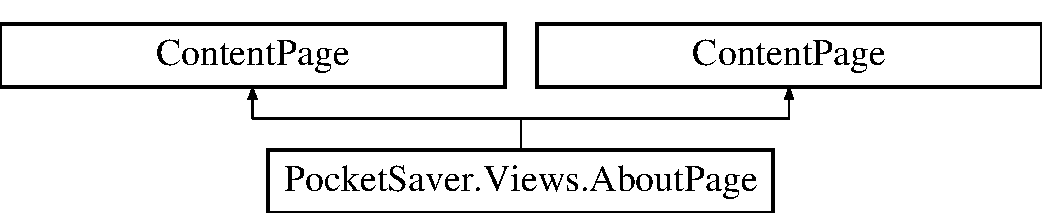
\includegraphics[height=2.000000cm]{class_pocket_saver_1_1_views_1_1_about_page}
\end{center}
\end{figure}
\subsection*{Public Member Functions}
\begin{DoxyCompactItemize}
\item 
\hyperlink{class_pocket_saver_1_1_views_1_1_about_page_af59ade4fd20fb646983154e0dbfd2f92}{About\+Page} ()
\begin{DoxyCompactList}\small\item\em Constructor for the \hyperlink{class_pocket_saver_1_1_views_1_1_about_page}{About\+Page} \end{DoxyCompactList}\end{DoxyCompactItemize}


\subsection{Detailed Description}
Class for the \hyperlink{class_pocket_saver_1_1_views_1_1_about_page}{About\+Page} 



\subsection{Constructor \& Destructor Documentation}
\mbox{\Hypertarget{class_pocket_saver_1_1_views_1_1_about_page_af59ade4fd20fb646983154e0dbfd2f92}\label{class_pocket_saver_1_1_views_1_1_about_page_af59ade4fd20fb646983154e0dbfd2f92}} 
\index{Pocket\+Saver\+::\+Views\+::\+About\+Page@{Pocket\+Saver\+::\+Views\+::\+About\+Page}!About\+Page@{About\+Page}}
\index{About\+Page@{About\+Page}!Pocket\+Saver\+::\+Views\+::\+About\+Page@{Pocket\+Saver\+::\+Views\+::\+About\+Page}}
\subsubsection{\texorpdfstring{About\+Page()}{AboutPage()}}
{\footnotesize\ttfamily Pocket\+Saver.\+Views.\+About\+Page.\+About\+Page (\begin{DoxyParamCaption}{ }\end{DoxyParamCaption})\hspace{0.3cm}{\ttfamily [inline]}}



Constructor for the \hyperlink{class_pocket_saver_1_1_views_1_1_about_page}{About\+Page} 



The documentation for this class was generated from the following files\+:\begin{DoxyCompactItemize}
\item 
C\+:/\+Users/\+Mevin/\+Pocket\+Saver/src/\+Pocket\+Saver/\+Pocket\+Saver/\+Pocket\+Saver/obj/\+Debug/Pocket\+Saver.\+Views.\+About\+Page.\+xaml.\+g.\+cs\item 
C\+:/\+Users/\+Mevin/\+Pocket\+Saver/src/\+Pocket\+Saver/\+Pocket\+Saver/\+Pocket\+Saver/\+Views/About\+Page.\+xaml.\+cs\end{DoxyCompactItemize}

\hypertarget{class_pocket_saver_1_1_view_models_1_1_about_view_model}{}\section{Pocket\+Saver.\+View\+Models.\+About\+View\+Model Class Reference}
\label{class_pocket_saver_1_1_view_models_1_1_about_view_model}\index{Pocket\+Saver.\+View\+Models.\+About\+View\+Model@{Pocket\+Saver.\+View\+Models.\+About\+View\+Model}}
Inheritance diagram for Pocket\+Saver.\+View\+Models.\+About\+View\+Model\+:\begin{figure}[H]
\begin{center}
\leavevmode
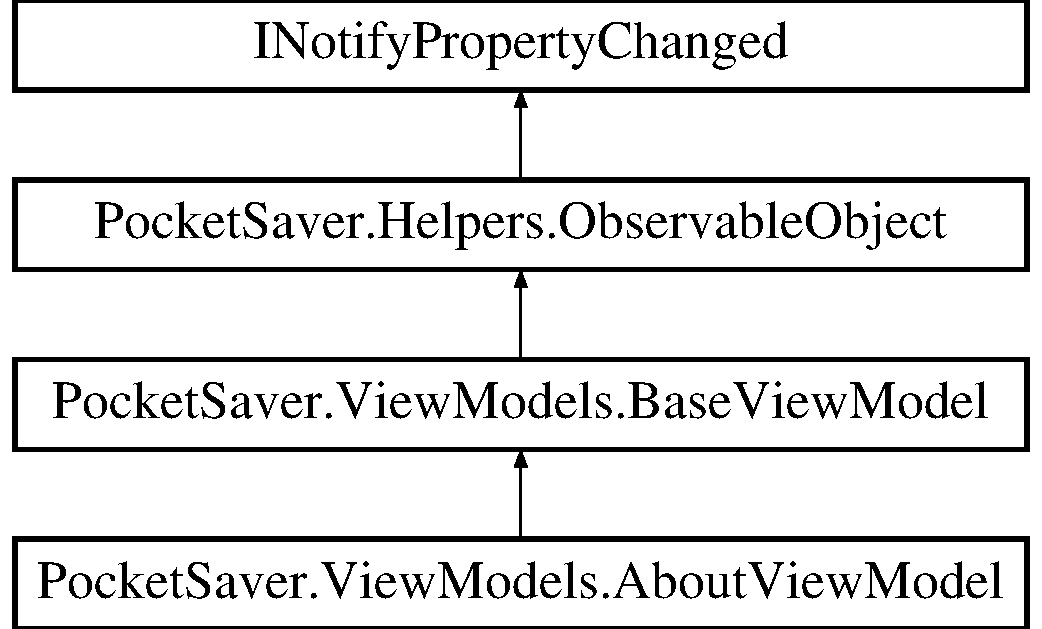
\includegraphics[height=4.000000cm]{class_pocket_saver_1_1_view_models_1_1_about_view_model}
\end{center}
\end{figure}
\subsection*{Properties}
\begin{DoxyCompactItemize}
\item 
I\+Command \hyperlink{class_pocket_saver_1_1_view_models_1_1_about_view_model_a05bca2ba82a3e0d0b231d177f3990e66}{Open\+Web\+Command}\hspace{0.3cm}{\ttfamily  \mbox{[}get\mbox{]}}
\begin{DoxyCompactList}\small\item\em Command to open browser to xamarin.\+com \end{DoxyCompactList}\end{DoxyCompactItemize}
\subsection*{Additional Inherited Members}


\subsection{Property Documentation}
\mbox{\Hypertarget{class_pocket_saver_1_1_view_models_1_1_about_view_model_a05bca2ba82a3e0d0b231d177f3990e66}\label{class_pocket_saver_1_1_view_models_1_1_about_view_model_a05bca2ba82a3e0d0b231d177f3990e66}} 
\index{Pocket\+Saver\+::\+View\+Models\+::\+About\+View\+Model@{Pocket\+Saver\+::\+View\+Models\+::\+About\+View\+Model}!Open\+Web\+Command@{Open\+Web\+Command}}
\index{Open\+Web\+Command@{Open\+Web\+Command}!Pocket\+Saver\+::\+View\+Models\+::\+About\+View\+Model@{Pocket\+Saver\+::\+View\+Models\+::\+About\+View\+Model}}
\subsubsection{\texorpdfstring{Open\+Web\+Command}{OpenWebCommand}}
{\footnotesize\ttfamily I\+Command Pocket\+Saver.\+View\+Models.\+About\+View\+Model.\+Open\+Web\+Command\hspace{0.3cm}{\ttfamily [get]}}



Command to open browser to xamarin.\+com 



The documentation for this class was generated from the following file\+:\begin{DoxyCompactItemize}
\item 
C\+:/\+Users/\+Mevin/\+Pocket\+Saver/src/\+Pocket\+Saver/\+Pocket\+Saver/\+Pocket\+Saver/\+View\+Models/About\+View\+Model.\+cs\end{DoxyCompactItemize}

\hypertarget{class_pocket_saver_1_1_services_1_1_api_s_v}{}\section{Pocket\+Saver.\+Services.\+Api\+SV Class Reference}
\label{class_pocket_saver_1_1_services_1_1_api_s_v}\index{Pocket\+Saver.\+Services.\+Api\+SV@{Pocket\+Saver.\+Services.\+Api\+SV}}


Class for the Api Service for the entire \hyperlink{namespace_pocket_saver}{Pocket\+Saver} Application. In this service, G\+ET, P\+O\+ST, P\+UT, and D\+E\+L\+E\+TE Methods are defined in a generic form for whatever Object the Database will return.  


\subsection*{Public Member Functions}
\begin{DoxyCompactItemize}
\item 
\hyperlink{class_pocket_saver_1_1_services_1_1_api_s_v_ab265e3f79436f302dde76459b6fefa46}{Api\+SV} ()
\begin{DoxyCompactList}\small\item\em Constructor for the \hyperlink{class_pocket_saver_1_1_services_1_1_api_s_v}{Api\+SV} which constructs the new H\+T\+TP Client and adds the default headers. \end{DoxyCompactList}\item 
String \hyperlink{class_pocket_saver_1_1_services_1_1_api_s_v_aa770136ecefc3ae66bff6dc75670df45}{Url\+Builder} (String query)
\begin{DoxyCompactList}\small\item\em Method used to create the U\+RL for the \hyperlink{class_pocket_saver_1_1_services_1_1_api_s_v}{Api\+SV} \end{DoxyCompactList}\item 
String \hyperlink{class_pocket_saver_1_1_services_1_1_api_s_v_aa5064fcb4a18768820f20c39d75d4d44}{Query\+Builder} (String query, String aggregate)
\begin{DoxyCompactList}\small\item\em Method used to create a query to the database. \end{DoxyCompactList}\item 
void \hyperlink{class_pocket_saver_1_1_services_1_1_api_s_v_a88eb168469465c1fcba4c25ce00c0204}{Http\+Body\+Builder$<$ T $>$} (T obj)
\begin{DoxyCompactList}\small\item\em Method used to create the Http\+Body of the P\+O\+ST Api request. \end{DoxyCompactList}\item 
async Task$<$ T $>$ \hyperlink{class_pocket_saver_1_1_services_1_1_api_s_v_af0ad1db31c39565bc5e46d7ef1985fbb}{Get$<$ T $>$} ()
\begin{DoxyCompactList}\small\item\em Api G\+ET Request method. \end{DoxyCompactList}\item 
async Task$<$ T $>$ \hyperlink{class_pocket_saver_1_1_services_1_1_api_s_v_a4db27f4d8526c13b6227e36f40e609e3}{Post$<$ T $>$} ()
\begin{DoxyCompactList}\small\item\em Api P\+O\+ST Request \end{DoxyCompactList}\item 
async Task$<$ T $>$ \hyperlink{class_pocket_saver_1_1_services_1_1_api_s_v_addfb96abb14d6189ad11040354540e08}{Put$<$ T $>$} ()
\begin{DoxyCompactList}\small\item\em Api P\+UT Request \end{DoxyCompactList}\item 
async Task$<$ T $>$ \hyperlink{class_pocket_saver_1_1_services_1_1_api_s_v_a1a4b1d8cc442dc1bcb908ff2ae7b243f}{Delete$<$ T $>$} ()
\begin{DoxyCompactList}\small\item\em Api D\+E\+L\+E\+TE Request \end{DoxyCompactList}\end{DoxyCompactItemize}
\subsection*{Properties}
\begin{DoxyCompactItemize}
\item 
\mbox{\Hypertarget{class_pocket_saver_1_1_services_1_1_api_s_v_a61c115b80ecb71b84cd31052aa876e4e}\label{class_pocket_saver_1_1_services_1_1_api_s_v_a61c115b80ecb71b84cd31052aa876e4e}} 
string {\bfseries url}\hspace{0.3cm}{\ttfamily  \mbox{[}get, set\mbox{]}}
\end{DoxyCompactItemize}


\subsection{Detailed Description}
Class for the Api Service for the entire \hyperlink{namespace_pocket_saver}{Pocket\+Saver} Application. In this service, G\+ET, P\+O\+ST, P\+UT, and D\+E\+L\+E\+TE Methods are defined in a generic form for whatever Object the Database will return. 



\subsection{Constructor \& Destructor Documentation}
\mbox{\Hypertarget{class_pocket_saver_1_1_services_1_1_api_s_v_ab265e3f79436f302dde76459b6fefa46}\label{class_pocket_saver_1_1_services_1_1_api_s_v_ab265e3f79436f302dde76459b6fefa46}} 
\index{Pocket\+Saver\+::\+Services\+::\+Api\+SV@{Pocket\+Saver\+::\+Services\+::\+Api\+SV}!Api\+SV@{Api\+SV}}
\index{Api\+SV@{Api\+SV}!Pocket\+Saver\+::\+Services\+::\+Api\+SV@{Pocket\+Saver\+::\+Services\+::\+Api\+SV}}
\subsubsection{\texorpdfstring{Api\+S\+V()}{ApiSV()}}
{\footnotesize\ttfamily Pocket\+Saver.\+Services.\+Api\+S\+V.\+Api\+SV (\begin{DoxyParamCaption}{ }\end{DoxyParamCaption})\hspace{0.3cm}{\ttfamily [inline]}}



Constructor for the \hyperlink{class_pocket_saver_1_1_services_1_1_api_s_v}{Api\+SV} which constructs the new H\+T\+TP Client and adds the default headers. 



\subsection{Member Function Documentation}
\mbox{\Hypertarget{class_pocket_saver_1_1_services_1_1_api_s_v_a1a4b1d8cc442dc1bcb908ff2ae7b243f}\label{class_pocket_saver_1_1_services_1_1_api_s_v_a1a4b1d8cc442dc1bcb908ff2ae7b243f}} 
\index{Pocket\+Saver\+::\+Services\+::\+Api\+SV@{Pocket\+Saver\+::\+Services\+::\+Api\+SV}!Delete$<$ T $>$@{Delete$<$ T $>$}}
\index{Delete$<$ T $>$@{Delete$<$ T $>$}!Pocket\+Saver\+::\+Services\+::\+Api\+SV@{Pocket\+Saver\+::\+Services\+::\+Api\+SV}}
\subsubsection{\texorpdfstring{Delete$<$ T $>$()}{Delete< T >()}}
{\footnotesize\ttfamily async Task$<$T$>$ Pocket\+Saver.\+Services.\+Api\+S\+V.\+Delete$<$ T $>$ (\begin{DoxyParamCaption}{ }\end{DoxyParamCaption})\hspace{0.3cm}{\ttfamily [inline]}}



Api D\+E\+L\+E\+TE Request 


\begin{DoxyTemplParams}{Template Parameters}
{\em T} & Model that the D\+E\+L\+E\+TE request will map to.\\
\hline
\end{DoxyTemplParams}
\begin{DoxyReturn}{Returns}
T Object that will be deleted by the Api Delete request.
\end{DoxyReturn}
\mbox{\Hypertarget{class_pocket_saver_1_1_services_1_1_api_s_v_af0ad1db31c39565bc5e46d7ef1985fbb}\label{class_pocket_saver_1_1_services_1_1_api_s_v_af0ad1db31c39565bc5e46d7ef1985fbb}} 
\index{Pocket\+Saver\+::\+Services\+::\+Api\+SV@{Pocket\+Saver\+::\+Services\+::\+Api\+SV}!Get$<$ T $>$@{Get$<$ T $>$}}
\index{Get$<$ T $>$@{Get$<$ T $>$}!Pocket\+Saver\+::\+Services\+::\+Api\+SV@{Pocket\+Saver\+::\+Services\+::\+Api\+SV}}
\subsubsection{\texorpdfstring{Get$<$ T $>$()}{Get< T >()}}
{\footnotesize\ttfamily async Task$<$T$>$ Pocket\+Saver.\+Services.\+Api\+S\+V.\+Get$<$ T $>$ (\begin{DoxyParamCaption}{ }\end{DoxyParamCaption})\hspace{0.3cm}{\ttfamily [inline]}}



Api G\+ET Request method. 


\begin{DoxyTemplParams}{Template Parameters}
{\em T} & Generic type T\\
\hline
\end{DoxyTemplParams}
\begin{DoxyReturn}{Returns}
T object retrieved from the Api request.
\end{DoxyReturn}
\mbox{\Hypertarget{class_pocket_saver_1_1_services_1_1_api_s_v_a88eb168469465c1fcba4c25ce00c0204}\label{class_pocket_saver_1_1_services_1_1_api_s_v_a88eb168469465c1fcba4c25ce00c0204}} 
\index{Pocket\+Saver\+::\+Services\+::\+Api\+SV@{Pocket\+Saver\+::\+Services\+::\+Api\+SV}!Http\+Body\+Builder$<$ T $>$@{Http\+Body\+Builder$<$ T $>$}}
\index{Http\+Body\+Builder$<$ T $>$@{Http\+Body\+Builder$<$ T $>$}!Pocket\+Saver\+::\+Services\+::\+Api\+SV@{Pocket\+Saver\+::\+Services\+::\+Api\+SV}}
\subsubsection{\texorpdfstring{Http\+Body\+Builder$<$ T $>$()}{HttpBodyBuilder< T >()}}
{\footnotesize\ttfamily void Pocket\+Saver.\+Services.\+Api\+S\+V.\+Http\+Body\+Builder$<$ T $>$ (\begin{DoxyParamCaption}\item[{T}]{obj }\end{DoxyParamCaption})\hspace{0.3cm}{\ttfamily [inline]}}



Method used to create the Http\+Body of the P\+O\+ST Api request. 


\begin{DoxyTemplParams}{Template Parameters}
{\em T} & T is a generic object to be used in the Http\+Body\\
\hline
\end{DoxyTemplParams}

\begin{DoxyParams}{Parameters}
{\em obj} & T object which will be serialized into a String\+Content object.\\
\hline
\end{DoxyParams}
\mbox{\Hypertarget{class_pocket_saver_1_1_services_1_1_api_s_v_a4db27f4d8526c13b6227e36f40e609e3}\label{class_pocket_saver_1_1_services_1_1_api_s_v_a4db27f4d8526c13b6227e36f40e609e3}} 
\index{Pocket\+Saver\+::\+Services\+::\+Api\+SV@{Pocket\+Saver\+::\+Services\+::\+Api\+SV}!Post$<$ T $>$@{Post$<$ T $>$}}
\index{Post$<$ T $>$@{Post$<$ T $>$}!Pocket\+Saver\+::\+Services\+::\+Api\+SV@{Pocket\+Saver\+::\+Services\+::\+Api\+SV}}
\subsubsection{\texorpdfstring{Post$<$ T $>$()}{Post< T >()}}
{\footnotesize\ttfamily async Task$<$T$>$ Pocket\+Saver.\+Services.\+Api\+S\+V.\+Post$<$ T $>$ (\begin{DoxyParamCaption}{ }\end{DoxyParamCaption})\hspace{0.3cm}{\ttfamily [inline]}}



Api P\+O\+ST Request 


\begin{DoxyTemplParams}{Template Parameters}
{\em T} & Model that the P\+O\+ST Request will map to.\\
\hline
\end{DoxyTemplParams}
\begin{DoxyReturn}{Returns}
T Object after successfully posting object to the Database.
\end{DoxyReturn}
\mbox{\Hypertarget{class_pocket_saver_1_1_services_1_1_api_s_v_addfb96abb14d6189ad11040354540e08}\label{class_pocket_saver_1_1_services_1_1_api_s_v_addfb96abb14d6189ad11040354540e08}} 
\index{Pocket\+Saver\+::\+Services\+::\+Api\+SV@{Pocket\+Saver\+::\+Services\+::\+Api\+SV}!Put$<$ T $>$@{Put$<$ T $>$}}
\index{Put$<$ T $>$@{Put$<$ T $>$}!Pocket\+Saver\+::\+Services\+::\+Api\+SV@{Pocket\+Saver\+::\+Services\+::\+Api\+SV}}
\subsubsection{\texorpdfstring{Put$<$ T $>$()}{Put< T >()}}
{\footnotesize\ttfamily async Task$<$T$>$ Pocket\+Saver.\+Services.\+Api\+S\+V.\+Put$<$ T $>$ (\begin{DoxyParamCaption}{ }\end{DoxyParamCaption})\hspace{0.3cm}{\ttfamily [inline]}}



Api P\+UT Request 


\begin{DoxyTemplParams}{Template Parameters}
{\em T} & Model that the P\+UT Request will map to.\\
\hline
\end{DoxyTemplParams}
\begin{DoxyReturn}{Returns}
Object T that is put into the database.
\end{DoxyReturn}
\mbox{\Hypertarget{class_pocket_saver_1_1_services_1_1_api_s_v_aa5064fcb4a18768820f20c39d75d4d44}\label{class_pocket_saver_1_1_services_1_1_api_s_v_aa5064fcb4a18768820f20c39d75d4d44}} 
\index{Pocket\+Saver\+::\+Services\+::\+Api\+SV@{Pocket\+Saver\+::\+Services\+::\+Api\+SV}!Query\+Builder@{Query\+Builder}}
\index{Query\+Builder@{Query\+Builder}!Pocket\+Saver\+::\+Services\+::\+Api\+SV@{Pocket\+Saver\+::\+Services\+::\+Api\+SV}}
\subsubsection{\texorpdfstring{Query\+Builder()}{QueryBuilder()}}
{\footnotesize\ttfamily String Pocket\+Saver.\+Services.\+Api\+S\+V.\+Query\+Builder (\begin{DoxyParamCaption}\item[{String}]{query,  }\item[{String}]{aggregate }\end{DoxyParamCaption})\hspace{0.3cm}{\ttfamily [inline]}}



Method used to create a query to the database. 


\begin{DoxyParams}{Parameters}
{\em query} & String for the query parameters to be added to the url.\\
\hline
{\em aggregate} & String for the aggregate queries to be added to the url.\\
\hline
\end{DoxyParams}
\begin{DoxyReturn}{Returns}
Final string with all query parameters to the database.
\end{DoxyReturn}
\mbox{\Hypertarget{class_pocket_saver_1_1_services_1_1_api_s_v_aa770136ecefc3ae66bff6dc75670df45}\label{class_pocket_saver_1_1_services_1_1_api_s_v_aa770136ecefc3ae66bff6dc75670df45}} 
\index{Pocket\+Saver\+::\+Services\+::\+Api\+SV@{Pocket\+Saver\+::\+Services\+::\+Api\+SV}!Url\+Builder@{Url\+Builder}}
\index{Url\+Builder@{Url\+Builder}!Pocket\+Saver\+::\+Services\+::\+Api\+SV@{Pocket\+Saver\+::\+Services\+::\+Api\+SV}}
\subsubsection{\texorpdfstring{Url\+Builder()}{UrlBuilder()}}
{\footnotesize\ttfamily String Pocket\+Saver.\+Services.\+Api\+S\+V.\+Url\+Builder (\begin{DoxyParamCaption}\item[{String}]{query }\end{DoxyParamCaption})\hspace{0.3cm}{\ttfamily [inline]}}



Method used to create the U\+RL for the \hyperlink{class_pocket_saver_1_1_services_1_1_api_s_v}{Api\+SV} 


\begin{DoxyParams}{Parameters}
{\em query} & String which is added to the end of the string for additional database queries\\
\hline
\end{DoxyParams}
\begin{DoxyReturn}{Returns}
String for the final url.
\end{DoxyReturn}


The documentation for this class was generated from the following file\+:\begin{DoxyCompactItemize}
\item 
C\+:/\+Users/\+Mevin/\+Pocket\+Saver/src/\+Pocket\+Saver/\+Pocket\+Saver/\+Pocket\+Saver/\+Services/Api\+S\+V.\+cs\end{DoxyCompactItemize}

\hypertarget{class_pocket_saver_1_1_app}{}\section{Pocket\+Saver.\+App Class Reference}
\label{class_pocket_saver_1_1_app}\index{Pocket\+Saver.\+App@{Pocket\+Saver.\+App}}
Inheritance diagram for Pocket\+Saver.\+App\+:\begin{figure}[H]
\begin{center}
\leavevmode
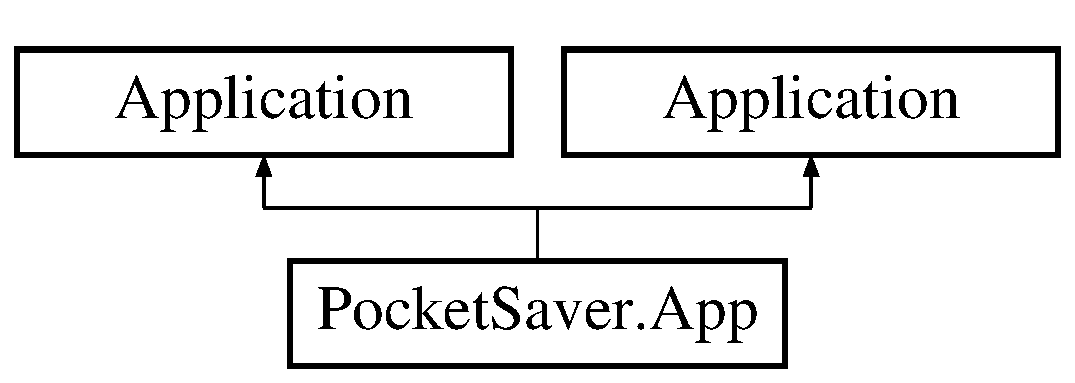
\includegraphics[height=2.000000cm]{class_pocket_saver_1_1_app}
\end{center}
\end{figure}
\subsection*{Static Public Member Functions}
\begin{DoxyCompactItemize}
\item 
\mbox{\Hypertarget{class_pocket_saver_1_1_app_a1ceff66a22060a629ba6db62fe1392a1}\label{class_pocket_saver_1_1_app_a1ceff66a22060a629ba6db62fe1392a1}} 
static void {\bfseries Set\+Main\+Page} ()
\item 
\mbox{\Hypertarget{class_pocket_saver_1_1_app_ab92761d9b4c322a99b3a0af0e32ccf53}\label{class_pocket_saver_1_1_app_ab92761d9b4c322a99b3a0af0e32ccf53}} 
static Page {\bfseries Get\+Main\+Page} ()
\end{DoxyCompactItemize}


The documentation for this class was generated from the following files\+:\begin{DoxyCompactItemize}
\item 
C\+:/\+Users/\+Mevin/\+Pocket\+Saver/src/\+Pocket\+Saver/\+Pocket\+Saver/\+Pocket\+Saver/App.\+xaml.\+cs\item 
C\+:/\+Users/\+Mevin/\+Pocket\+Saver/src/\+Pocket\+Saver/\+Pocket\+Saver/\+Pocket\+Saver/obj/\+Debug/Pocket\+Saver.\+App.\+xaml.\+g.\+cs\end{DoxyCompactItemize}

\hypertarget{class_pocket_saver_1_1_models_1_1_base_data_object}{}\section{Pocket\+Saver.\+Models.\+Base\+Data\+Object Class Reference}
\label{class_pocket_saver_1_1_models_1_1_base_data_object}\index{Pocket\+Saver.\+Models.\+Base\+Data\+Object@{Pocket\+Saver.\+Models.\+Base\+Data\+Object}}
Inheritance diagram for Pocket\+Saver.\+Models.\+Base\+Data\+Object\+:\begin{figure}[H]
\begin{center}
\leavevmode
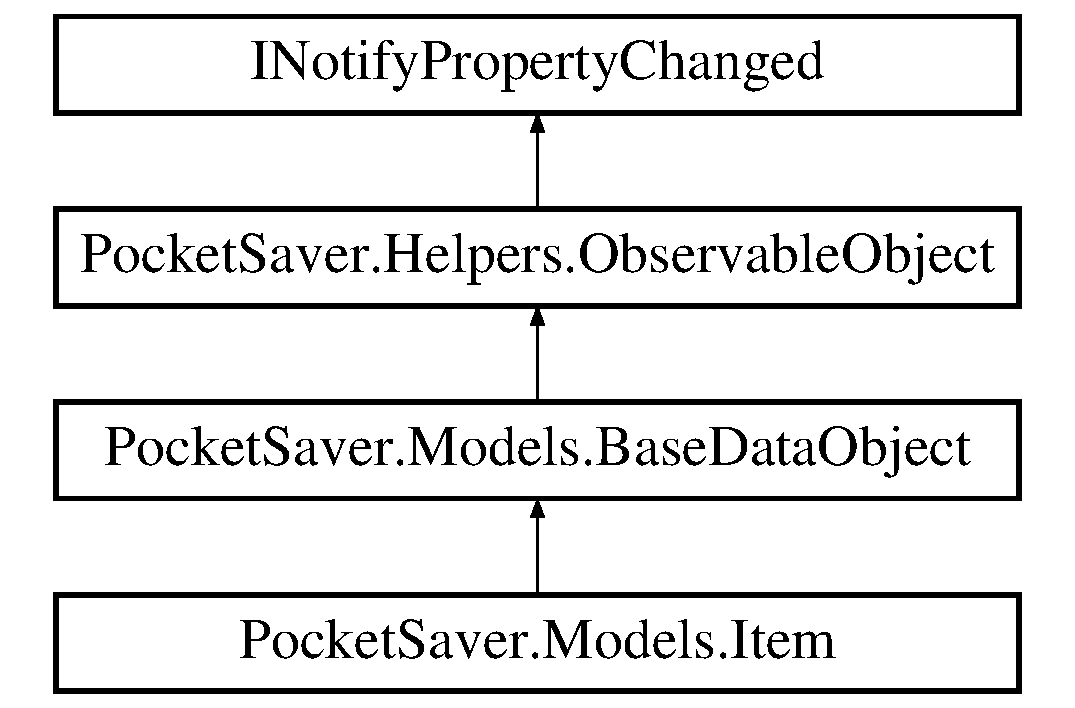
\includegraphics[height=4.000000cm]{class_pocket_saver_1_1_models_1_1_base_data_object}
\end{center}
\end{figure}
\subsection*{Properties}
\begin{DoxyCompactItemize}
\item 
string \hyperlink{class_pocket_saver_1_1_models_1_1_base_data_object_ab4303cb60bc268e37fda9a6b9d1b3987}{Id}\hspace{0.3cm}{\ttfamily  \mbox{[}get, set\mbox{]}}
\begin{DoxyCompactList}\small\item\em Id for item \end{DoxyCompactList}\item 
Date\+Time\+Offset \hyperlink{class_pocket_saver_1_1_models_1_1_base_data_object_a7e190cdd8cf97ceb371c81dc26bf27cb}{Created\+At}\hspace{0.3cm}{\ttfamily  \mbox{[}get, set\mbox{]}}
\begin{DoxyCompactList}\small\item\em Azure created at time stamp \end{DoxyCompactList}\item 
Date\+Time\+Offset \hyperlink{class_pocket_saver_1_1_models_1_1_base_data_object_ad4f722a084f206961d65507e3f29750c}{Updated\+At}\hspace{0.3cm}{\ttfamily  \mbox{[}get, set\mbox{]}}
\begin{DoxyCompactList}\small\item\em Azure Update\+At timestamp for online/offline sync \end{DoxyCompactList}\item 
string \hyperlink{class_pocket_saver_1_1_models_1_1_base_data_object_ad6a1af4f7f1b9a24e6ea2561b78948b6}{Azure\+Version}\hspace{0.3cm}{\ttfamily  \mbox{[}get, set\mbox{]}}
\begin{DoxyCompactList}\small\item\em Azure version for online/offline sync \end{DoxyCompactList}\end{DoxyCompactItemize}
\subsection*{Additional Inherited Members}


\subsection{Property Documentation}
\mbox{\Hypertarget{class_pocket_saver_1_1_models_1_1_base_data_object_ad6a1af4f7f1b9a24e6ea2561b78948b6}\label{class_pocket_saver_1_1_models_1_1_base_data_object_ad6a1af4f7f1b9a24e6ea2561b78948b6}} 
\index{Pocket\+Saver\+::\+Models\+::\+Base\+Data\+Object@{Pocket\+Saver\+::\+Models\+::\+Base\+Data\+Object}!Azure\+Version@{Azure\+Version}}
\index{Azure\+Version@{Azure\+Version}!Pocket\+Saver\+::\+Models\+::\+Base\+Data\+Object@{Pocket\+Saver\+::\+Models\+::\+Base\+Data\+Object}}
\subsubsection{\texorpdfstring{Azure\+Version}{AzureVersion}}
{\footnotesize\ttfamily string Pocket\+Saver.\+Models.\+Base\+Data\+Object.\+Azure\+Version\hspace{0.3cm}{\ttfamily [get]}, {\ttfamily [set]}}



Azure version for online/offline sync 

\mbox{\Hypertarget{class_pocket_saver_1_1_models_1_1_base_data_object_a7e190cdd8cf97ceb371c81dc26bf27cb}\label{class_pocket_saver_1_1_models_1_1_base_data_object_a7e190cdd8cf97ceb371c81dc26bf27cb}} 
\index{Pocket\+Saver\+::\+Models\+::\+Base\+Data\+Object@{Pocket\+Saver\+::\+Models\+::\+Base\+Data\+Object}!Created\+At@{Created\+At}}
\index{Created\+At@{Created\+At}!Pocket\+Saver\+::\+Models\+::\+Base\+Data\+Object@{Pocket\+Saver\+::\+Models\+::\+Base\+Data\+Object}}
\subsubsection{\texorpdfstring{Created\+At}{CreatedAt}}
{\footnotesize\ttfamily Date\+Time\+Offset Pocket\+Saver.\+Models.\+Base\+Data\+Object.\+Created\+At\hspace{0.3cm}{\ttfamily [get]}, {\ttfamily [set]}}



Azure created at time stamp 

\mbox{\Hypertarget{class_pocket_saver_1_1_models_1_1_base_data_object_ab4303cb60bc268e37fda9a6b9d1b3987}\label{class_pocket_saver_1_1_models_1_1_base_data_object_ab4303cb60bc268e37fda9a6b9d1b3987}} 
\index{Pocket\+Saver\+::\+Models\+::\+Base\+Data\+Object@{Pocket\+Saver\+::\+Models\+::\+Base\+Data\+Object}!Id@{Id}}
\index{Id@{Id}!Pocket\+Saver\+::\+Models\+::\+Base\+Data\+Object@{Pocket\+Saver\+::\+Models\+::\+Base\+Data\+Object}}
\subsubsection{\texorpdfstring{Id}{Id}}
{\footnotesize\ttfamily string Pocket\+Saver.\+Models.\+Base\+Data\+Object.\+Id\hspace{0.3cm}{\ttfamily [get]}, {\ttfamily [set]}}



Id for item 

\mbox{\Hypertarget{class_pocket_saver_1_1_models_1_1_base_data_object_ad4f722a084f206961d65507e3f29750c}\label{class_pocket_saver_1_1_models_1_1_base_data_object_ad4f722a084f206961d65507e3f29750c}} 
\index{Pocket\+Saver\+::\+Models\+::\+Base\+Data\+Object@{Pocket\+Saver\+::\+Models\+::\+Base\+Data\+Object}!Updated\+At@{Updated\+At}}
\index{Updated\+At@{Updated\+At}!Pocket\+Saver\+::\+Models\+::\+Base\+Data\+Object@{Pocket\+Saver\+::\+Models\+::\+Base\+Data\+Object}}
\subsubsection{\texorpdfstring{Updated\+At}{UpdatedAt}}
{\footnotesize\ttfamily Date\+Time\+Offset Pocket\+Saver.\+Models.\+Base\+Data\+Object.\+Updated\+At\hspace{0.3cm}{\ttfamily [get]}, {\ttfamily [set]}}



Azure Update\+At timestamp for online/offline sync 



The documentation for this class was generated from the following file\+:\begin{DoxyCompactItemize}
\item 
C\+:/\+Users/\+Mevin/\+Pocket\+Saver/src/\+Pocket\+Saver/\+Pocket\+Saver/\+Pocket\+Saver/\+Services/\+Models/Base\+Data\+Object.\+cs\end{DoxyCompactItemize}

\hypertarget{class_pocket_saver_1_1_view_models_1_1_base_view_model}{}\section{Pocket\+Saver.\+View\+Models.\+Base\+View\+Model Class Reference}
\label{class_pocket_saver_1_1_view_models_1_1_base_view_model}\index{Pocket\+Saver.\+View\+Models.\+Base\+View\+Model@{Pocket\+Saver.\+View\+Models.\+Base\+View\+Model}}
Inheritance diagram for Pocket\+Saver.\+View\+Models.\+Base\+View\+Model\+:\begin{figure}[H]
\begin{center}
\leavevmode
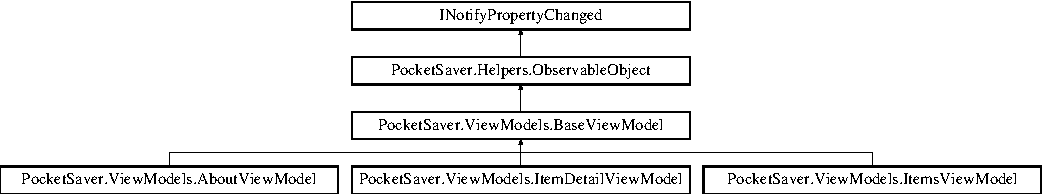
\includegraphics[height=2.610723cm]{class_pocket_saver_1_1_view_models_1_1_base_view_model}
\end{center}
\end{figure}
\subsection*{Public Attributes}
\begin{DoxyCompactItemize}
\item 
\hyperlink{interface_pocket_saver_1_1_services_1_1_i_data_store}{I\+Data\+Store}$<$ \hyperlink{class_pocket_saver_1_1_models_1_1_item}{Item} $>$ \hyperlink{class_pocket_saver_1_1_view_models_1_1_base_view_model_aa9bdaa0ab23edb66ede005d03cb871f8}{Data\+Store} =$>$ Dependency\+Service.\+Get$<$\hyperlink{interface_pocket_saver_1_1_services_1_1_i_data_store}{I\+Data\+Store}$<$\hyperlink{class_pocket_saver_1_1_models_1_1_item}{Item}$>$$>$()
\begin{DoxyCompactList}\small\item\em Get the azure service instance \end{DoxyCompactList}\end{DoxyCompactItemize}
\subsection*{Properties}
\begin{DoxyCompactItemize}
\item 
\mbox{\Hypertarget{class_pocket_saver_1_1_view_models_1_1_base_view_model_a81ff71c4b4b506f92c30ade18f312957}\label{class_pocket_saver_1_1_view_models_1_1_base_view_model_a81ff71c4b4b506f92c30ade18f312957}} 
bool {\bfseries Is\+Busy}\hspace{0.3cm}{\ttfamily  \mbox{[}get, set\mbox{]}}
\item 
string \hyperlink{class_pocket_saver_1_1_view_models_1_1_base_view_model_a0113530f15cb67f44568bc7ec3c44695}{Title}\hspace{0.3cm}{\ttfamily  \mbox{[}get, set\mbox{]}}
\begin{DoxyCompactList}\small\item\em Public property to set and get the title of the item \end{DoxyCompactList}\end{DoxyCompactItemize}
\subsection*{Additional Inherited Members}


\subsection{Member Data Documentation}
\mbox{\Hypertarget{class_pocket_saver_1_1_view_models_1_1_base_view_model_aa9bdaa0ab23edb66ede005d03cb871f8}\label{class_pocket_saver_1_1_view_models_1_1_base_view_model_aa9bdaa0ab23edb66ede005d03cb871f8}} 
\index{Pocket\+Saver\+::\+View\+Models\+::\+Base\+View\+Model@{Pocket\+Saver\+::\+View\+Models\+::\+Base\+View\+Model}!Data\+Store@{Data\+Store}}
\index{Data\+Store@{Data\+Store}!Pocket\+Saver\+::\+View\+Models\+::\+Base\+View\+Model@{Pocket\+Saver\+::\+View\+Models\+::\+Base\+View\+Model}}
\subsubsection{\texorpdfstring{Data\+Store}{DataStore}}
{\footnotesize\ttfamily \hyperlink{interface_pocket_saver_1_1_services_1_1_i_data_store}{I\+Data\+Store}$<$\hyperlink{class_pocket_saver_1_1_models_1_1_item}{Item}$>$ Pocket\+Saver.\+View\+Models.\+Base\+View\+Model.\+Data\+Store =$>$ Dependency\+Service.\+Get$<$\hyperlink{interface_pocket_saver_1_1_services_1_1_i_data_store}{I\+Data\+Store}$<$\hyperlink{class_pocket_saver_1_1_models_1_1_item}{Item}$>$$>$()}



Get the azure service instance 



\subsection{Property Documentation}
\mbox{\Hypertarget{class_pocket_saver_1_1_view_models_1_1_base_view_model_a0113530f15cb67f44568bc7ec3c44695}\label{class_pocket_saver_1_1_view_models_1_1_base_view_model_a0113530f15cb67f44568bc7ec3c44695}} 
\index{Pocket\+Saver\+::\+View\+Models\+::\+Base\+View\+Model@{Pocket\+Saver\+::\+View\+Models\+::\+Base\+View\+Model}!Title@{Title}}
\index{Title@{Title}!Pocket\+Saver\+::\+View\+Models\+::\+Base\+View\+Model@{Pocket\+Saver\+::\+View\+Models\+::\+Base\+View\+Model}}
\subsubsection{\texorpdfstring{Title}{Title}}
{\footnotesize\ttfamily string Pocket\+Saver.\+View\+Models.\+Base\+View\+Model.\+Title\hspace{0.3cm}{\ttfamily [get]}, {\ttfamily [set]}}



Public property to set and get the title of the item 



The documentation for this class was generated from the following file\+:\begin{DoxyCompactItemize}
\item 
C\+:/\+Users/\+Mevin/\+Pocket\+Saver/src/\+Pocket\+Saver/\+Pocket\+Saver/\+Pocket\+Saver/\+View\+Models/Base\+View\+Model.\+cs\end{DoxyCompactItemize}

\hypertarget{class_pocket_saver_1_1_services_1_1_models_1_1_common_return_model}{}\section{Pocket\+Saver.\+Services.\+Models.\+Common\+Return\+Model Class Reference}
\label{class_pocket_saver_1_1_services_1_1_models_1_1_common_return_model}\index{Pocket\+Saver.\+Services.\+Models.\+Common\+Return\+Model@{Pocket\+Saver.\+Services.\+Models.\+Common\+Return\+Model}}
\subsection*{Properties}
\begin{DoxyCompactItemize}
\item 
\mbox{\Hypertarget{class_pocket_saver_1_1_services_1_1_models_1_1_common_return_model_a5576a42cbc2c7860a69e9f8953a628e0}\label{class_pocket_saver_1_1_services_1_1_models_1_1_common_return_model_a5576a42cbc2c7860a69e9f8953a628e0}} 
Object {\bfseries results}\hspace{0.3cm}{\ttfamily  \mbox{[}get, set\mbox{]}}
\end{DoxyCompactItemize}


The documentation for this class was generated from the following file\+:\begin{DoxyCompactItemize}
\item 
C\+:/\+Users/\+Mevin/\+Pocket\+Saver/src/\+Pocket\+Saver/\+Pocket\+Saver/\+Pocket\+Saver/\+Services/\+Models/Common\+Return\+Model.\+cs\end{DoxyCompactItemize}

\hypertarget{class_pocket_saver_1_1_helpers_1_1_custom_image_cell}{}\section{Pocket\+Saver.\+Helpers.\+Custom\+Image\+Cell Class Reference}
\label{class_pocket_saver_1_1_helpers_1_1_custom_image_cell}\index{Pocket\+Saver.\+Helpers.\+Custom\+Image\+Cell@{Pocket\+Saver.\+Helpers.\+Custom\+Image\+Cell}}


Class for a Custom Image\+Cell that allows for tinted images.  


Inheritance diagram for Pocket\+Saver.\+Helpers.\+Custom\+Image\+Cell\+:\begin{figure}[H]
\begin{center}
\leavevmode
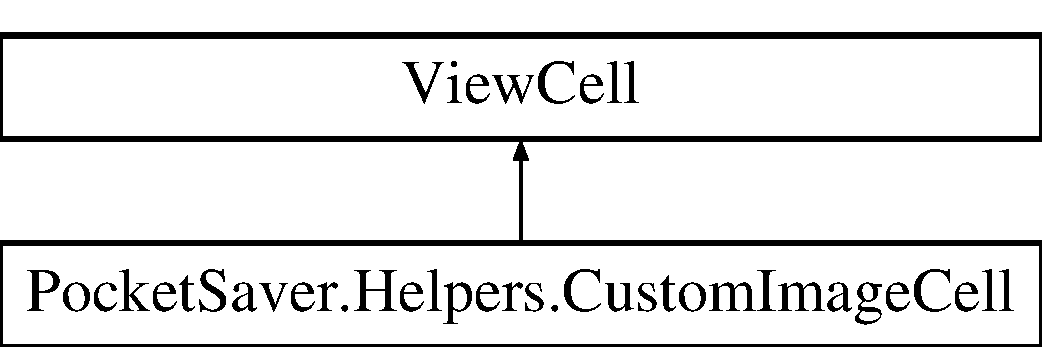
\includegraphics[height=2.000000cm]{class_pocket_saver_1_1_helpers_1_1_custom_image_cell}
\end{center}
\end{figure}
\subsection*{Static Public Attributes}
\begin{DoxyCompactItemize}
\item 
\mbox{\Hypertarget{class_pocket_saver_1_1_helpers_1_1_custom_image_cell_aea48b309b2352d8e1bd0956385d1ad75}\label{class_pocket_saver_1_1_helpers_1_1_custom_image_cell_aea48b309b2352d8e1bd0956385d1ad75}} 
static readonly Bindable\+Property {\bfseries Image\+Source\+Property} = Bindable\+Property.\+Create(nameof(Image\+Source), typeof(string), typeof(\hyperlink{class_pocket_saver_1_1_helpers_1_1_custom_image_cell}{Custom\+Image\+Cell}), \char`\"{}\char`\"{})
\item 
\mbox{\Hypertarget{class_pocket_saver_1_1_helpers_1_1_custom_image_cell_a8ecfcf21a28f0e562af4a1057b2812ef}\label{class_pocket_saver_1_1_helpers_1_1_custom_image_cell_a8ecfcf21a28f0e562af4a1057b2812ef}} 
static readonly Bindable\+Property {\bfseries Text\+Property} = Bindable\+Property.\+Create(nameof(Text), typeof(string), typeof(\hyperlink{class_pocket_saver_1_1_helpers_1_1_custom_image_cell}{Custom\+Image\+Cell}), \char`\"{}\char`\"{})
\item 
\mbox{\Hypertarget{class_pocket_saver_1_1_helpers_1_1_custom_image_cell_a1a0959726ac43e4edce8835071be4919}\label{class_pocket_saver_1_1_helpers_1_1_custom_image_cell_a1a0959726ac43e4edce8835071be4919}} 
static readonly Bindable\+Property {\bfseries Tint\+Color\+Property} = Bindable\+Property.\+Create(nameof(Tint\+Color), typeof(Color), typeof(\hyperlink{class_pocket_saver_1_1_helpers_1_1_custom_image_cell}{Custom\+Image\+Cell}), Color.\+Black)
\item 
\mbox{\Hypertarget{class_pocket_saver_1_1_helpers_1_1_custom_image_cell_a8b14499e269b99078270681080a0c3a2}\label{class_pocket_saver_1_1_helpers_1_1_custom_image_cell_a8b14499e269b99078270681080a0c3a2}} 
static readonly Bindable\+Property {\bfseries Text\+Color\+Property} = Bindable\+Property.\+Create(nameof(Text\+Color), typeof(Color), typeof(\hyperlink{class_pocket_saver_1_1_helpers_1_1_custom_image_cell}{Custom\+Image\+Cell}), Color.\+Black)
\end{DoxyCompactItemize}
\subsection*{Protected Member Functions}
\begin{DoxyCompactItemize}
\item 
\mbox{\Hypertarget{class_pocket_saver_1_1_helpers_1_1_custom_image_cell_a50f823444df75ae279914e413ec2ae89}\label{class_pocket_saver_1_1_helpers_1_1_custom_image_cell_a50f823444df75ae279914e413ec2ae89}} 
override void {\bfseries On\+Binding\+Context\+Changed} ()
\end{DoxyCompactItemize}
\subsection*{Properties}
\begin{DoxyCompactItemize}
\item 
\mbox{\Hypertarget{class_pocket_saver_1_1_helpers_1_1_custom_image_cell_a2a0cc37177f6a8d568cd12e0a8e0e46c}\label{class_pocket_saver_1_1_helpers_1_1_custom_image_cell_a2a0cc37177f6a8d568cd12e0a8e0e46c}} 
string {\bfseries Image\+Source}\hspace{0.3cm}{\ttfamily  \mbox{[}get, set\mbox{]}}
\item 
\mbox{\Hypertarget{class_pocket_saver_1_1_helpers_1_1_custom_image_cell_a392bbbe5b2c146ff0b52b7476e0aabc7}\label{class_pocket_saver_1_1_helpers_1_1_custom_image_cell_a392bbbe5b2c146ff0b52b7476e0aabc7}} 
string {\bfseries Text}\hspace{0.3cm}{\ttfamily  \mbox{[}get, set\mbox{]}}
\item 
\mbox{\Hypertarget{class_pocket_saver_1_1_helpers_1_1_custom_image_cell_a7e60b02d00da82b47de972b574d7dd17}\label{class_pocket_saver_1_1_helpers_1_1_custom_image_cell_a7e60b02d00da82b47de972b574d7dd17}} 
Color {\bfseries Tint\+Color}\hspace{0.3cm}{\ttfamily  \mbox{[}get, set\mbox{]}}
\item 
\mbox{\Hypertarget{class_pocket_saver_1_1_helpers_1_1_custom_image_cell_a2e64dc3584ba512b306b58c487aaba17}\label{class_pocket_saver_1_1_helpers_1_1_custom_image_cell_a2e64dc3584ba512b306b58c487aaba17}} 
Color {\bfseries Text\+Color}\hspace{0.3cm}{\ttfamily  \mbox{[}get, set\mbox{]}}
\end{DoxyCompactItemize}


\subsection{Detailed Description}
Class for a Custom Image\+Cell that allows for tinted images. 



The documentation for this class was generated from the following file\+:\begin{DoxyCompactItemize}
\item 
C\+:/\+Users/\+Mevin/\+Pocket\+Saver/src/\+Pocket\+Saver/\+Pocket\+Saver/\+Pocket\+Saver/\+Helpers/Custom\+Image\+Cell.\+cs\end{DoxyCompactItemize}

\hypertarget{class_pocket_saver_1_1_models_1_1_grouped_master_page_item}{}\section{Pocket\+Saver.\+Models.\+Grouped\+Master\+Page\+Item Class Reference}
\label{class_pocket_saver_1_1_models_1_1_grouped_master_page_item}\index{Pocket\+Saver.\+Models.\+Grouped\+Master\+Page\+Item@{Pocket\+Saver.\+Models.\+Grouped\+Master\+Page\+Item}}
Inheritance diagram for Pocket\+Saver.\+Models.\+Grouped\+Master\+Page\+Item\+:\begin{figure}[H]
\begin{center}
\leavevmode
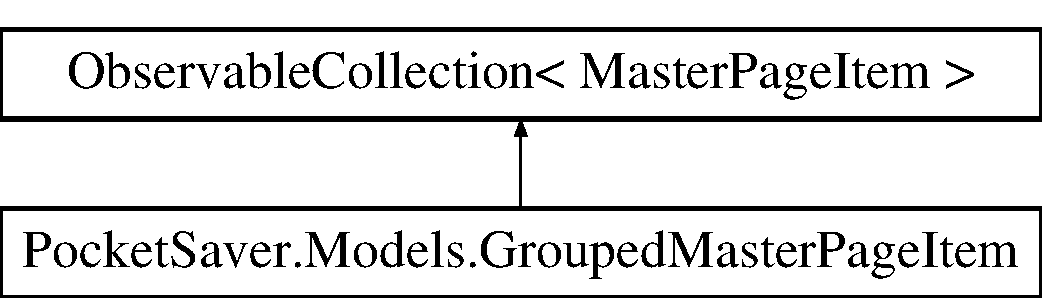
\includegraphics[height=2.000000cm]{class_pocket_saver_1_1_models_1_1_grouped_master_page_item}
\end{center}
\end{figure}
\subsection*{Properties}
\begin{DoxyCompactItemize}
\item 
\mbox{\Hypertarget{class_pocket_saver_1_1_models_1_1_grouped_master_page_item_a619204fd7ed3f9066387189fae76a98d}\label{class_pocket_saver_1_1_models_1_1_grouped_master_page_item_a619204fd7ed3f9066387189fae76a98d}} 
string {\bfseries Long\+Name}\hspace{0.3cm}{\ttfamily  \mbox{[}get, set\mbox{]}}
\item 
\mbox{\Hypertarget{class_pocket_saver_1_1_models_1_1_grouped_master_page_item_a696caaaeb0bff26534f64905fa6e61be}\label{class_pocket_saver_1_1_models_1_1_grouped_master_page_item_a696caaaeb0bff26534f64905fa6e61be}} 
string {\bfseries Grouping}\hspace{0.3cm}{\ttfamily  \mbox{[}get, set\mbox{]}}
\end{DoxyCompactItemize}


The documentation for this class was generated from the following file\+:\begin{DoxyCompactItemize}
\item 
C\+:/\+Users/\+Mevin/\+Pocket\+Saver/src/\+Pocket\+Saver/\+Pocket\+Saver/\+Pocket\+Saver/\+Services/\+Models/Master\+Page\+Item.\+cs\end{DoxyCompactItemize}

\hypertarget{class_pocket_saver_1_1_views_1_1_home_1_1_home_page}{}\section{Pocket\+Saver.\+Views.\+Home.\+Home\+Page Class Reference}
\label{class_pocket_saver_1_1_views_1_1_home_1_1_home_page}\index{Pocket\+Saver.\+Views.\+Home.\+Home\+Page@{Pocket\+Saver.\+Views.\+Home.\+Home\+Page}}


Class for the \hyperlink{class_pocket_saver_1_1_views_1_1_home_1_1_home_page}{Home\+Page} View.  


Inheritance diagram for Pocket\+Saver.\+Views.\+Home.\+Home\+Page\+:\begin{figure}[H]
\begin{center}
\leavevmode
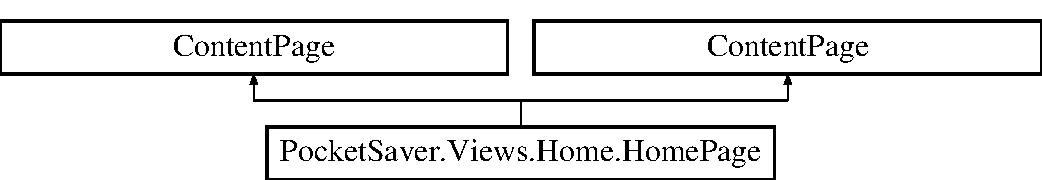
\includegraphics[height=2.000000cm]{class_pocket_saver_1_1_views_1_1_home_1_1_home_page}
\end{center}
\end{figure}
\subsection*{Public Member Functions}
\begin{DoxyCompactItemize}
\item 
\hyperlink{class_pocket_saver_1_1_views_1_1_home_1_1_home_page_a816da50c9151c39febfe0f5803a2cdb3}{Home\+Page} ()
\begin{DoxyCompactList}\small\item\em Constructor for the \hyperlink{class_pocket_saver_1_1_views_1_1_home_1_1_home_page}{Home\+Page} View. \end{DoxyCompactList}\end{DoxyCompactItemize}
\subsection*{Static Public Attributes}
\begin{DoxyCompactItemize}
\item 
static Observable\+Collection$<$ String $>$ \hyperlink{class_pocket_saver_1_1_views_1_1_home_1_1_home_page_a3304f2eabf76bd2855aa806363a9616d}{month\+List}
\begin{DoxyCompactList}\small\item\em Creating variables to be used in the class. \end{DoxyCompactList}\end{DoxyCompactItemize}
\subsection*{Protected Member Functions}
\begin{DoxyCompactItemize}
\item 
async override void \hyperlink{class_pocket_saver_1_1_views_1_1_home_1_1_home_page_a47aecb7aa46d3e9e22867599a254b478}{On\+Appearing} ()
\begin{DoxyCompactList}\small\item\em On\+Appearing method that calls View\+Model to prepare totals. \end{DoxyCompactList}\end{DoxyCompactItemize}


\subsection{Detailed Description}
Class for the \hyperlink{class_pocket_saver_1_1_views_1_1_home_1_1_home_page}{Home\+Page} View. 



\subsection{Constructor \& Destructor Documentation}
\mbox{\Hypertarget{class_pocket_saver_1_1_views_1_1_home_1_1_home_page_a816da50c9151c39febfe0f5803a2cdb3}\label{class_pocket_saver_1_1_views_1_1_home_1_1_home_page_a816da50c9151c39febfe0f5803a2cdb3}} 
\index{Pocket\+Saver\+::\+Views\+::\+Home\+::\+Home\+Page@{Pocket\+Saver\+::\+Views\+::\+Home\+::\+Home\+Page}!Home\+Page@{Home\+Page}}
\index{Home\+Page@{Home\+Page}!Pocket\+Saver\+::\+Views\+::\+Home\+::\+Home\+Page@{Pocket\+Saver\+::\+Views\+::\+Home\+::\+Home\+Page}}
\subsubsection{\texorpdfstring{Home\+Page()}{HomePage()}}
{\footnotesize\ttfamily Pocket\+Saver.\+Views.\+Home.\+Home\+Page.\+Home\+Page (\begin{DoxyParamCaption}{ }\end{DoxyParamCaption})\hspace{0.3cm}{\ttfamily [inline]}}



Constructor for the \hyperlink{class_pocket_saver_1_1_views_1_1_home_1_1_home_page}{Home\+Page} View. 



\subsection{Member Function Documentation}
\mbox{\Hypertarget{class_pocket_saver_1_1_views_1_1_home_1_1_home_page_a47aecb7aa46d3e9e22867599a254b478}\label{class_pocket_saver_1_1_views_1_1_home_1_1_home_page_a47aecb7aa46d3e9e22867599a254b478}} 
\index{Pocket\+Saver\+::\+Views\+::\+Home\+::\+Home\+Page@{Pocket\+Saver\+::\+Views\+::\+Home\+::\+Home\+Page}!On\+Appearing@{On\+Appearing}}
\index{On\+Appearing@{On\+Appearing}!Pocket\+Saver\+::\+Views\+::\+Home\+::\+Home\+Page@{Pocket\+Saver\+::\+Views\+::\+Home\+::\+Home\+Page}}
\subsubsection{\texorpdfstring{On\+Appearing()}{OnAppearing()}}
{\footnotesize\ttfamily async override void Pocket\+Saver.\+Views.\+Home.\+Home\+Page.\+On\+Appearing (\begin{DoxyParamCaption}{ }\end{DoxyParamCaption})\hspace{0.3cm}{\ttfamily [inline]}, {\ttfamily [protected]}}



On\+Appearing method that calls View\+Model to prepare totals. 



\subsection{Member Data Documentation}
\mbox{\Hypertarget{class_pocket_saver_1_1_views_1_1_home_1_1_home_page_a3304f2eabf76bd2855aa806363a9616d}\label{class_pocket_saver_1_1_views_1_1_home_1_1_home_page_a3304f2eabf76bd2855aa806363a9616d}} 
\index{Pocket\+Saver\+::\+Views\+::\+Home\+::\+Home\+Page@{Pocket\+Saver\+::\+Views\+::\+Home\+::\+Home\+Page}!month\+List@{month\+List}}
\index{month\+List@{month\+List}!Pocket\+Saver\+::\+Views\+::\+Home\+::\+Home\+Page@{Pocket\+Saver\+::\+Views\+::\+Home\+::\+Home\+Page}}
\subsubsection{\texorpdfstring{month\+List}{monthList}}
{\footnotesize\ttfamily Observable\+Collection$<$String$>$ Pocket\+Saver.\+Views.\+Home.\+Home\+Page.\+month\+List\hspace{0.3cm}{\ttfamily [static]}}



Creating variables to be used in the class. 



The documentation for this class was generated from the following files\+:\begin{DoxyCompactItemize}
\item 
C\+:/\+Users/\+Mevin/\+Pocket\+Saver/src/\+Pocket\+Saver/\+Pocket\+Saver/\+Pocket\+Saver/obj/\+Debug/Pocket\+Saver.\+Views.\+Home.\+Home\+Page.\+xaml.\+g.\+cs\item 
C\+:/\+Users/\+Mevin/\+Pocket\+Saver/src/\+Pocket\+Saver/\+Pocket\+Saver/\+Pocket\+Saver/\+Views/\+Home/Home\+Page.\+xaml.\+cs\end{DoxyCompactItemize}

\hypertarget{interface_pocket_saver_1_1_services_1_1_i_data_store}{}\section{Pocket\+Saver.\+Services.\+I\+Data\+Store$<$ T $>$ Interface Template Reference}
\label{interface_pocket_saver_1_1_services_1_1_i_data_store}\index{Pocket\+Saver.\+Services.\+I\+Data\+Store$<$ T $>$@{Pocket\+Saver.\+Services.\+I\+Data\+Store$<$ T $>$}}
\subsection*{Public Member Functions}
\begin{DoxyCompactItemize}
\item 
\mbox{\Hypertarget{interface_pocket_saver_1_1_services_1_1_i_data_store_a352d3b450114de4e698ba1c39c479e65}\label{interface_pocket_saver_1_1_services_1_1_i_data_store_a352d3b450114de4e698ba1c39c479e65}} 
Task$<$ bool $>$ {\bfseries Add\+Item\+Async} (T item)
\item 
\mbox{\Hypertarget{interface_pocket_saver_1_1_services_1_1_i_data_store_aede96600f1b62b1524c953a1dc7aa82a}\label{interface_pocket_saver_1_1_services_1_1_i_data_store_aede96600f1b62b1524c953a1dc7aa82a}} 
Task$<$ bool $>$ {\bfseries Update\+Item\+Async} (T item)
\item 
\mbox{\Hypertarget{interface_pocket_saver_1_1_services_1_1_i_data_store_a3ac0c2a4527346de3171d1dc9952b0a7}\label{interface_pocket_saver_1_1_services_1_1_i_data_store_a3ac0c2a4527346de3171d1dc9952b0a7}} 
Task$<$ bool $>$ {\bfseries Delete\+Item\+Async} (T item)
\item 
\mbox{\Hypertarget{interface_pocket_saver_1_1_services_1_1_i_data_store_a35c05f2290db4c5d1a2658b2e640d532}\label{interface_pocket_saver_1_1_services_1_1_i_data_store_a35c05f2290db4c5d1a2658b2e640d532}} 
Task$<$ T $>$ {\bfseries Get\+Item\+Async} (string id)
\item 
\mbox{\Hypertarget{interface_pocket_saver_1_1_services_1_1_i_data_store_a2c7f92ed596bfa467b57ec135f008e44}\label{interface_pocket_saver_1_1_services_1_1_i_data_store_a2c7f92ed596bfa467b57ec135f008e44}} 
Task$<$ I\+Enumerable$<$ T $>$ $>$ {\bfseries Get\+Items\+Async} (bool force\+Refresh=false)
\item 
\mbox{\Hypertarget{interface_pocket_saver_1_1_services_1_1_i_data_store_a60e7759eb8483ebae451559003aa2dbb}\label{interface_pocket_saver_1_1_services_1_1_i_data_store_a60e7759eb8483ebae451559003aa2dbb}} 
Task {\bfseries Initialize\+Async} ()
\item 
\mbox{\Hypertarget{interface_pocket_saver_1_1_services_1_1_i_data_store_ad1a85284ff0d25e60454d37335905519}\label{interface_pocket_saver_1_1_services_1_1_i_data_store_ad1a85284ff0d25e60454d37335905519}} 
Task$<$ bool $>$ {\bfseries Pull\+Latest\+Async} ()
\item 
\mbox{\Hypertarget{interface_pocket_saver_1_1_services_1_1_i_data_store_a1d31fca2d28005ac878c1a16fbb16fa1}\label{interface_pocket_saver_1_1_services_1_1_i_data_store_a1d31fca2d28005ac878c1a16fbb16fa1}} 
Task$<$ bool $>$ {\bfseries Sync\+Async} ()
\end{DoxyCompactItemize}


The documentation for this interface was generated from the following file\+:\begin{DoxyCompactItemize}
\item 
C\+:/\+Users/\+Mevin/\+Pocket\+Saver/src/\+Pocket\+Saver/\+Pocket\+Saver/\+Pocket\+Saver/\+Services/I\+Data\+Store.\+cs\end{DoxyCompactItemize}

\hypertarget{class_pocket_saver_1_1_models_1_1_item}{}\section{Pocket\+Saver.\+Models.\+Item Class Reference}
\label{class_pocket_saver_1_1_models_1_1_item}\index{Pocket\+Saver.\+Models.\+Item@{Pocket\+Saver.\+Models.\+Item}}
Inheritance diagram for Pocket\+Saver.\+Models.\+Item\+:\begin{figure}[H]
\begin{center}
\leavevmode
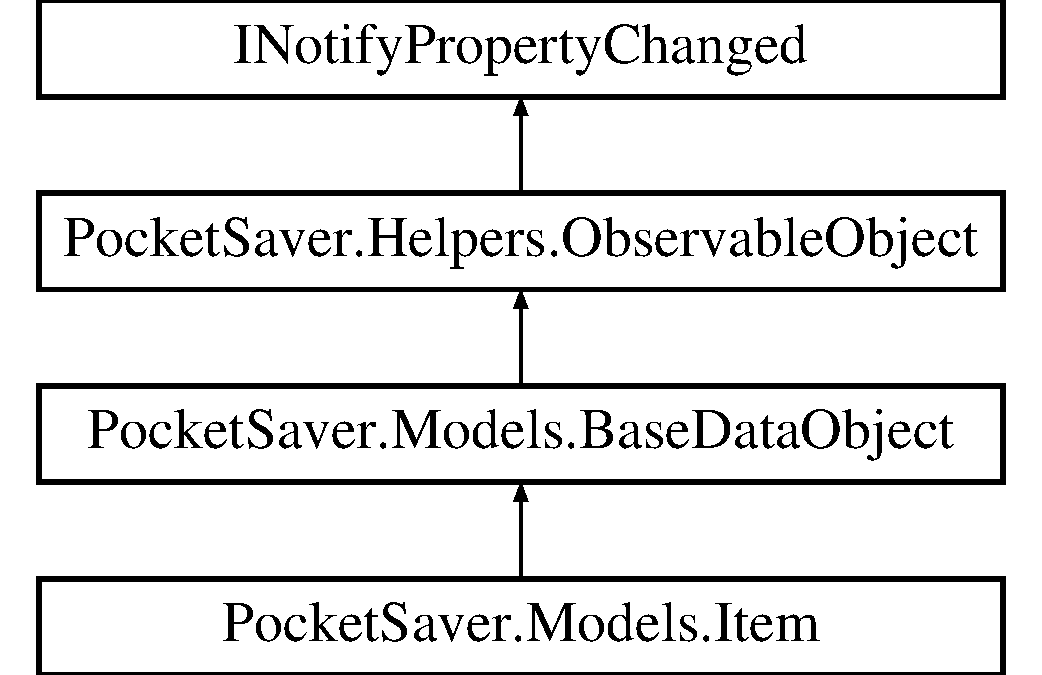
\includegraphics[height=4.000000cm]{class_pocket_saver_1_1_models_1_1_item}
\end{center}
\end{figure}
\subsection*{Properties}
\begin{DoxyCompactItemize}
\item 
\mbox{\Hypertarget{class_pocket_saver_1_1_models_1_1_item_a31de729c01ebd81d1014b89715b0302e}\label{class_pocket_saver_1_1_models_1_1_item_a31de729c01ebd81d1014b89715b0302e}} 
string {\bfseries Text}\hspace{0.3cm}{\ttfamily  \mbox{[}get, set\mbox{]}}
\item 
\mbox{\Hypertarget{class_pocket_saver_1_1_models_1_1_item_a826ed24319ef431f685e6957fc5da8c3}\label{class_pocket_saver_1_1_models_1_1_item_a826ed24319ef431f685e6957fc5da8c3}} 
string {\bfseries Description}\hspace{0.3cm}{\ttfamily  \mbox{[}get, set\mbox{]}}
\end{DoxyCompactItemize}
\subsection*{Additional Inherited Members}


The documentation for this class was generated from the following file\+:\begin{DoxyCompactItemize}
\item 
C\+:/\+Users/\+Mevin/\+Pocket\+Saver/src/\+Pocket\+Saver/\+Pocket\+Saver/\+Pocket\+Saver/\+Services/\+Models/Item.\+cs\end{DoxyCompactItemize}

\hypertarget{class_pocket_saver_1_1_views_1_1_item_detail_page}{}\section{Pocket\+Saver.\+Views.\+Item\+Detail\+Page Class Reference}
\label{class_pocket_saver_1_1_views_1_1_item_detail_page}\index{Pocket\+Saver.\+Views.\+Item\+Detail\+Page@{Pocket\+Saver.\+Views.\+Item\+Detail\+Page}}
Inheritance diagram for Pocket\+Saver.\+Views.\+Item\+Detail\+Page\+:\begin{figure}[H]
\begin{center}
\leavevmode
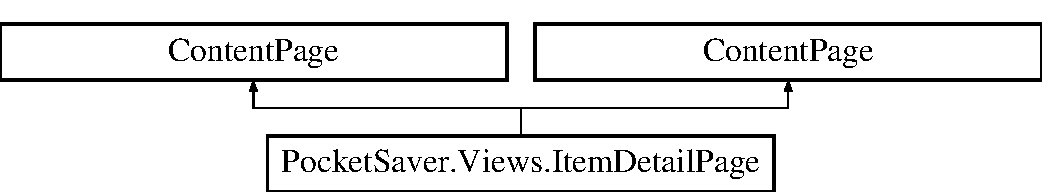
\includegraphics[height=2.000000cm]{class_pocket_saver_1_1_views_1_1_item_detail_page}
\end{center}
\end{figure}
\subsection*{Public Member Functions}
\begin{DoxyCompactItemize}
\item 
\mbox{\Hypertarget{class_pocket_saver_1_1_views_1_1_item_detail_page_ae6e0fbb25aceb544eb1c2c9a1e5abe9e}\label{class_pocket_saver_1_1_views_1_1_item_detail_page_ae6e0fbb25aceb544eb1c2c9a1e5abe9e}} 
{\bfseries Item\+Detail\+Page} (\hyperlink{class_pocket_saver_1_1_view_models_1_1_item_detail_view_model}{Item\+Detail\+View\+Model} view\+Model)
\end{DoxyCompactItemize}


The documentation for this class was generated from the following files\+:\begin{DoxyCompactItemize}
\item 
C\+:/\+Users/\+Mevin/\+Pocket\+Saver/src/\+Pocket\+Saver/\+Pocket\+Saver/\+Pocket\+Saver/obj/\+Debug/Pocket\+Saver.\+Views.\+Item\+Detail\+Page.\+xaml.\+g.\+cs\item 
C\+:/\+Users/\+Mevin/\+Pocket\+Saver/src/\+Pocket\+Saver/\+Pocket\+Saver/\+Pocket\+Saver/\+Views/Item\+Detail\+Page.\+xaml.\+cs\end{DoxyCompactItemize}

\hypertarget{class_pocket_saver_1_1_view_models_1_1_item_detail_view_model}{}\section{Pocket\+Saver.\+View\+Models.\+Item\+Detail\+View\+Model Class Reference}
\label{class_pocket_saver_1_1_view_models_1_1_item_detail_view_model}\index{Pocket\+Saver.\+View\+Models.\+Item\+Detail\+View\+Model@{Pocket\+Saver.\+View\+Models.\+Item\+Detail\+View\+Model}}
Inheritance diagram for Pocket\+Saver.\+View\+Models.\+Item\+Detail\+View\+Model\+:\begin{figure}[H]
\begin{center}
\leavevmode
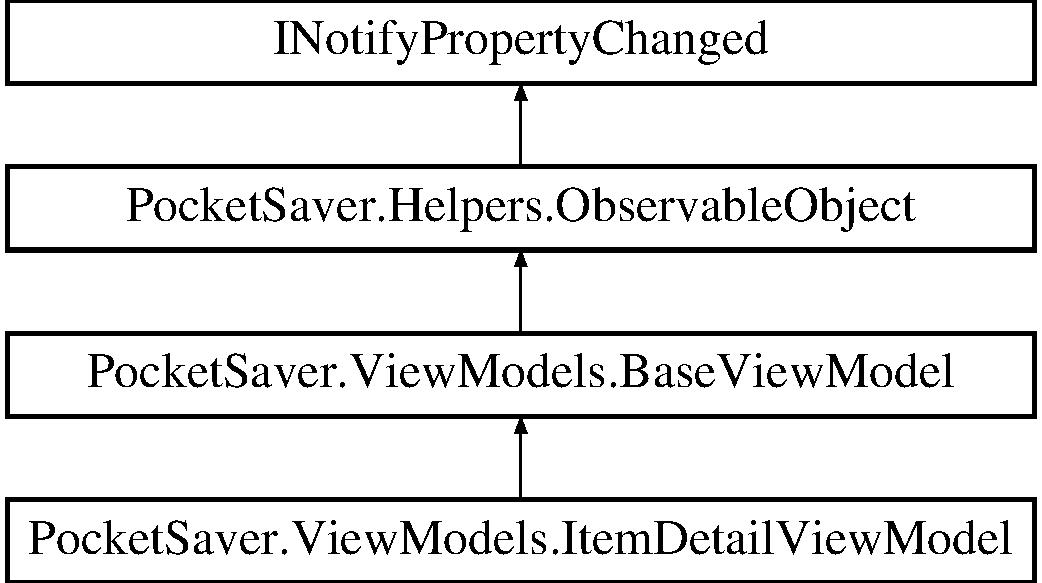
\includegraphics[height=4.000000cm]{class_pocket_saver_1_1_view_models_1_1_item_detail_view_model}
\end{center}
\end{figure}
\subsection*{Public Member Functions}
\begin{DoxyCompactItemize}
\item 
\mbox{\Hypertarget{class_pocket_saver_1_1_view_models_1_1_item_detail_view_model_af1d90985e2d67dfab6222c901004d0e1}\label{class_pocket_saver_1_1_view_models_1_1_item_detail_view_model_af1d90985e2d67dfab6222c901004d0e1}} 
{\bfseries Item\+Detail\+View\+Model} (\hyperlink{class_pocket_saver_1_1_models_1_1_item}{Item} item=null)
\end{DoxyCompactItemize}
\subsection*{Properties}
\begin{DoxyCompactItemize}
\item 
\mbox{\Hypertarget{class_pocket_saver_1_1_view_models_1_1_item_detail_view_model_a47380690257d441f6e430422f620b7ba}\label{class_pocket_saver_1_1_view_models_1_1_item_detail_view_model_a47380690257d441f6e430422f620b7ba}} 
\hyperlink{class_pocket_saver_1_1_models_1_1_item}{Item} {\bfseries Item}\hspace{0.3cm}{\ttfamily  \mbox{[}get, set\mbox{]}}
\item 
\mbox{\Hypertarget{class_pocket_saver_1_1_view_models_1_1_item_detail_view_model_a34c5b071c8ae1be0160b67007b308a51}\label{class_pocket_saver_1_1_view_models_1_1_item_detail_view_model_a34c5b071c8ae1be0160b67007b308a51}} 
int {\bfseries Quantity}\hspace{0.3cm}{\ttfamily  \mbox{[}get, set\mbox{]}}
\end{DoxyCompactItemize}
\subsection*{Additional Inherited Members}


The documentation for this class was generated from the following file\+:\begin{DoxyCompactItemize}
\item 
C\+:/\+Users/\+Mevin/\+Pocket\+Saver/src/\+Pocket\+Saver/\+Pocket\+Saver/\+Pocket\+Saver/\+View\+Models/Item\+Detail\+View\+Model.\+cs\end{DoxyCompactItemize}

\hypertarget{class_pocket_saver_1_1_views_1_1_items_page}{}\section{Pocket\+Saver.\+Views.\+Items\+Page Class Reference}
\label{class_pocket_saver_1_1_views_1_1_items_page}\index{Pocket\+Saver.\+Views.\+Items\+Page@{Pocket\+Saver.\+Views.\+Items\+Page}}
Inheritance diagram for Pocket\+Saver.\+Views.\+Items\+Page\+:\begin{figure}[H]
\begin{center}
\leavevmode
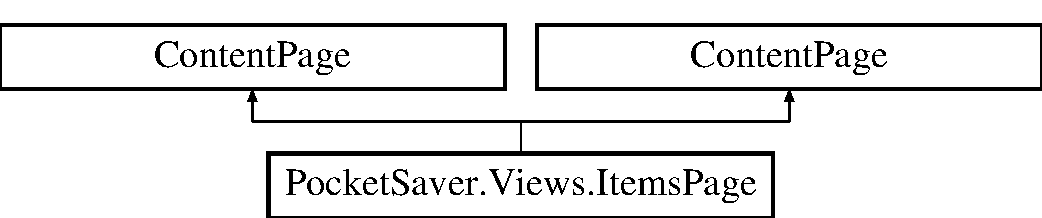
\includegraphics[height=2.000000cm]{class_pocket_saver_1_1_views_1_1_items_page}
\end{center}
\end{figure}
\subsection*{Protected Member Functions}
\begin{DoxyCompactItemize}
\item 
\mbox{\Hypertarget{class_pocket_saver_1_1_views_1_1_items_page_acab1e8c0784e7ea4116250dcc902ef32}\label{class_pocket_saver_1_1_views_1_1_items_page_acab1e8c0784e7ea4116250dcc902ef32}} 
override void {\bfseries On\+Appearing} ()
\end{DoxyCompactItemize}


The documentation for this class was generated from the following files\+:\begin{DoxyCompactItemize}
\item 
C\+:/\+Users/\+Mevin/\+Pocket\+Saver/src/\+Pocket\+Saver/\+Pocket\+Saver/\+Pocket\+Saver/obj/\+Debug/Pocket\+Saver.\+Views.\+Items\+Page.\+xaml.\+g.\+cs\item 
C\+:/\+Users/\+Mevin/\+Pocket\+Saver/src/\+Pocket\+Saver/\+Pocket\+Saver/\+Pocket\+Saver/\+Views/Items\+Page.\+xaml.\+cs\end{DoxyCompactItemize}

\hypertarget{class_pocket_saver_1_1_view_models_1_1_items_view_model}{}\section{Pocket\+Saver.\+View\+Models.\+Items\+View\+Model Class Reference}
\label{class_pocket_saver_1_1_view_models_1_1_items_view_model}\index{Pocket\+Saver.\+View\+Models.\+Items\+View\+Model@{Pocket\+Saver.\+View\+Models.\+Items\+View\+Model}}
Inheritance diagram for Pocket\+Saver.\+View\+Models.\+Items\+View\+Model\+:\begin{figure}[H]
\begin{center}
\leavevmode
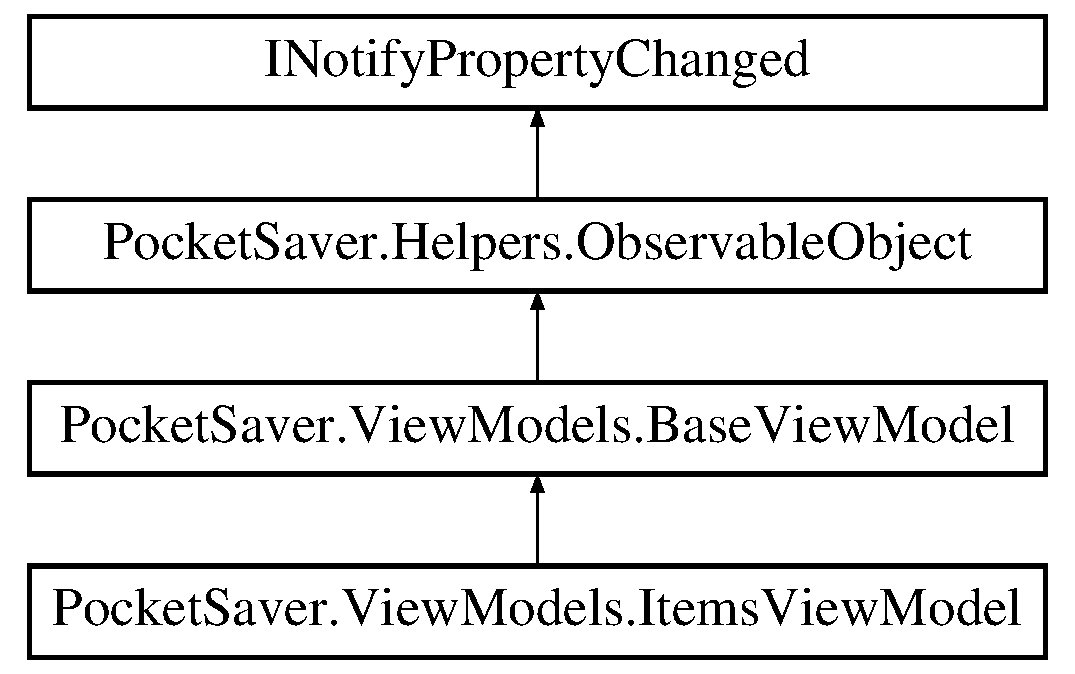
\includegraphics[height=4.000000cm]{class_pocket_saver_1_1_view_models_1_1_items_view_model}
\end{center}
\end{figure}
\subsection*{Properties}
\begin{DoxyCompactItemize}
\item 
\mbox{\Hypertarget{class_pocket_saver_1_1_view_models_1_1_items_view_model_a617da1e419ddadb0a751d66a7ba0822f}\label{class_pocket_saver_1_1_view_models_1_1_items_view_model_a617da1e419ddadb0a751d66a7ba0822f}} 
\hyperlink{class_pocket_saver_1_1_helpers_1_1_observable_range_collection}{Observable\+Range\+Collection}$<$ \hyperlink{class_pocket_saver_1_1_models_1_1_item}{Item} $>$ {\bfseries Items}\hspace{0.3cm}{\ttfamily  \mbox{[}get, set\mbox{]}}
\item 
\mbox{\Hypertarget{class_pocket_saver_1_1_view_models_1_1_items_view_model_af0317819948c9e0306beb71aadab21be}\label{class_pocket_saver_1_1_view_models_1_1_items_view_model_af0317819948c9e0306beb71aadab21be}} 
Command {\bfseries Load\+Items\+Command}\hspace{0.3cm}{\ttfamily  \mbox{[}get, set\mbox{]}}
\end{DoxyCompactItemize}
\subsection*{Additional Inherited Members}


The documentation for this class was generated from the following file\+:\begin{DoxyCompactItemize}
\item 
C\+:/\+Users/\+Mevin/\+Pocket\+Saver/src/\+Pocket\+Saver/\+Pocket\+Saver/\+Pocket\+Saver/\+View\+Models/Items\+View\+Model.\+cs\end{DoxyCompactItemize}

\hypertarget{class_pocket_saver_1_1_views_1_1_main_master_detail_page}{}\section{Pocket\+Saver.\+Views.\+Main\+Master\+Detail\+Page Class Reference}
\label{class_pocket_saver_1_1_views_1_1_main_master_detail_page}\index{Pocket\+Saver.\+Views.\+Main\+Master\+Detail\+Page@{Pocket\+Saver.\+Views.\+Main\+Master\+Detail\+Page}}


Class for the Master\+Detail page.  


Inheritance diagram for Pocket\+Saver.\+Views.\+Main\+Master\+Detail\+Page\+:\begin{figure}[H]
\begin{center}
\leavevmode
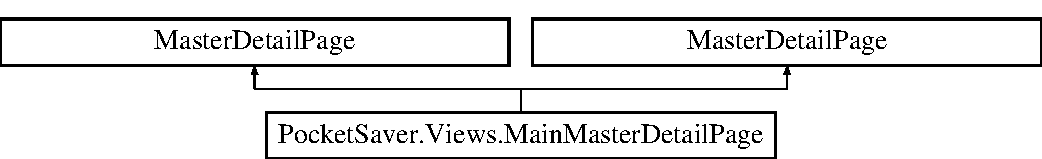
\includegraphics[height=2.000000cm]{class_pocket_saver_1_1_views_1_1_main_master_detail_page}
\end{center}
\end{figure}
\subsection*{Public Member Functions}
\begin{DoxyCompactItemize}
\item 
\hyperlink{class_pocket_saver_1_1_views_1_1_main_master_detail_page_ac8ec8ea55d0c0c111d1c58255406f16f}{Main\+Master\+Detail\+Page} ()
\begin{DoxyCompactList}\small\item\em Constructor for the \hyperlink{class_pocket_saver_1_1_views_1_1_main_master_detail_page}{Main\+Master\+Detail\+Page}. \end{DoxyCompactList}\item 
\mbox{\Hypertarget{class_pocket_saver_1_1_views_1_1_main_master_detail_page_a5350164e6e86879fc93ba9821459eccf}\label{class_pocket_saver_1_1_views_1_1_main_master_detail_page_a5350164e6e86879fc93ba9821459eccf}} 
void {\bfseries Navigate\+To} (Page page)
\end{DoxyCompactItemize}


\subsection{Detailed Description}
Class for the Master\+Detail page. 



\subsection{Constructor \& Destructor Documentation}
\mbox{\Hypertarget{class_pocket_saver_1_1_views_1_1_main_master_detail_page_ac8ec8ea55d0c0c111d1c58255406f16f}\label{class_pocket_saver_1_1_views_1_1_main_master_detail_page_ac8ec8ea55d0c0c111d1c58255406f16f}} 
\index{Pocket\+Saver\+::\+Views\+::\+Main\+Master\+Detail\+Page@{Pocket\+Saver\+::\+Views\+::\+Main\+Master\+Detail\+Page}!Main\+Master\+Detail\+Page@{Main\+Master\+Detail\+Page}}
\index{Main\+Master\+Detail\+Page@{Main\+Master\+Detail\+Page}!Pocket\+Saver\+::\+Views\+::\+Main\+Master\+Detail\+Page@{Pocket\+Saver\+::\+Views\+::\+Main\+Master\+Detail\+Page}}
\subsubsection{\texorpdfstring{Main\+Master\+Detail\+Page()}{MainMasterDetailPage()}}
{\footnotesize\ttfamily Pocket\+Saver.\+Views.\+Main\+Master\+Detail\+Page.\+Main\+Master\+Detail\+Page (\begin{DoxyParamCaption}{ }\end{DoxyParamCaption})\hspace{0.3cm}{\ttfamily [inline]}}



Constructor for the \hyperlink{class_pocket_saver_1_1_views_1_1_main_master_detail_page}{Main\+Master\+Detail\+Page}. 



The documentation for this class was generated from the following files\+:\begin{DoxyCompactItemize}
\item 
C\+:/\+Users/\+Mevin/\+Pocket\+Saver/src/\+Pocket\+Saver/\+Pocket\+Saver/\+Pocket\+Saver/obj/\+Debug/Pocket\+Saver.\+Views.\+Main\+Master\+Detail\+Page.\+xaml.\+g.\+cs\item 
C\+:/\+Users/\+Mevin/\+Pocket\+Saver/src/\+Pocket\+Saver/\+Pocket\+Saver/\+Pocket\+Saver/\+Views/Main\+Master\+Detail\+Page.\+xaml.\+cs\end{DoxyCompactItemize}

\hypertarget{class_pocket_saver_1_1_views_1_1_main_menu_page}{}\section{Pocket\+Saver.\+Views.\+Main\+Menu\+Page Class Reference}
\label{class_pocket_saver_1_1_views_1_1_main_menu_page}\index{Pocket\+Saver.\+Views.\+Main\+Menu\+Page@{Pocket\+Saver.\+Views.\+Main\+Menu\+Page}}


Class for the Main\+Menu page.  


Inheritance diagram for Pocket\+Saver.\+Views.\+Main\+Menu\+Page\+:\begin{figure}[H]
\begin{center}
\leavevmode
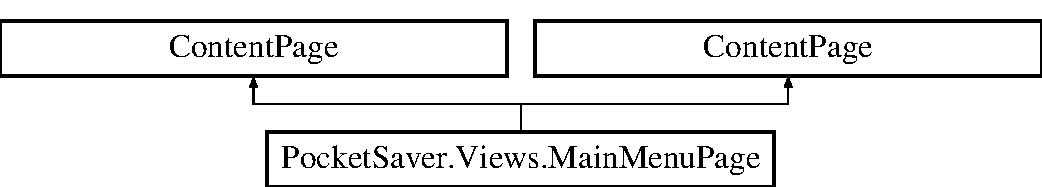
\includegraphics[height=2.000000cm]{class_pocket_saver_1_1_views_1_1_main_menu_page}
\end{center}
\end{figure}
\subsection*{Public Member Functions}
\begin{DoxyCompactItemize}
\item 
\hyperlink{class_pocket_saver_1_1_views_1_1_main_menu_page_aee8c6fc4d2a5fb1f7ee53f9175d2c84d}{Main\+Menu\+Page} ()
\begin{DoxyCompactList}\small\item\em Constructor for the Main\+Menu page. \end{DoxyCompactList}\end{DoxyCompactItemize}
\subsection*{Properties}
\begin{DoxyCompactItemize}
\item 
\mbox{\Hypertarget{class_pocket_saver_1_1_views_1_1_main_menu_page_a9abb113a5c4417cd6072bb967b8aa98d}\label{class_pocket_saver_1_1_views_1_1_main_menu_page_a9abb113a5c4417cd6072bb967b8aa98d}} 
List\+View {\bfseries List\+View}\hspace{0.3cm}{\ttfamily  \mbox{[}get\mbox{]}}
\end{DoxyCompactItemize}


\subsection{Detailed Description}
Class for the Main\+Menu page. 



\subsection{Constructor \& Destructor Documentation}
\mbox{\Hypertarget{class_pocket_saver_1_1_views_1_1_main_menu_page_aee8c6fc4d2a5fb1f7ee53f9175d2c84d}\label{class_pocket_saver_1_1_views_1_1_main_menu_page_aee8c6fc4d2a5fb1f7ee53f9175d2c84d}} 
\index{Pocket\+Saver\+::\+Views\+::\+Main\+Menu\+Page@{Pocket\+Saver\+::\+Views\+::\+Main\+Menu\+Page}!Main\+Menu\+Page@{Main\+Menu\+Page}}
\index{Main\+Menu\+Page@{Main\+Menu\+Page}!Pocket\+Saver\+::\+Views\+::\+Main\+Menu\+Page@{Pocket\+Saver\+::\+Views\+::\+Main\+Menu\+Page}}
\subsubsection{\texorpdfstring{Main\+Menu\+Page()}{MainMenuPage()}}
{\footnotesize\ttfamily Pocket\+Saver.\+Views.\+Main\+Menu\+Page.\+Main\+Menu\+Page (\begin{DoxyParamCaption}{ }\end{DoxyParamCaption})\hspace{0.3cm}{\ttfamily [inline]}}



Constructor for the Main\+Menu page. 



The documentation for this class was generated from the following files\+:\begin{DoxyCompactItemize}
\item 
C\+:/\+Users/\+Mevin/\+Pocket\+Saver/src/\+Pocket\+Saver/\+Pocket\+Saver/\+Pocket\+Saver/obj/\+Debug/Pocket\+Saver.\+Views.\+Main\+Menu\+Page.\+xaml.\+g.\+cs\item 
C\+:/\+Users/\+Mevin/\+Pocket\+Saver/src/\+Pocket\+Saver/\+Pocket\+Saver/\+Pocket\+Saver/\+Views/Main\+Menu\+Page.\+xaml.\+cs\end{DoxyCompactItemize}

\hypertarget{class_pocket_saver_1_1_models_1_1_master_page_item}{}\section{Pocket\+Saver.\+Models.\+Master\+Page\+Item Class Reference}
\label{class_pocket_saver_1_1_models_1_1_master_page_item}\index{Pocket\+Saver.\+Models.\+Master\+Page\+Item@{Pocket\+Saver.\+Models.\+Master\+Page\+Item}}


Class for the \hyperlink{class_pocket_saver_1_1_models_1_1_master_page_item}{Master\+Page\+Item} to be used for the Main\+Menu  


\subsection*{Properties}
\begin{DoxyCompactItemize}
\item 
\mbox{\Hypertarget{class_pocket_saver_1_1_models_1_1_master_page_item_a7c4154175a757c8f49d03383ea4ada42}\label{class_pocket_saver_1_1_models_1_1_master_page_item_a7c4154175a757c8f49d03383ea4ada42}} 
string {\bfseries Title}\hspace{0.3cm}{\ttfamily  \mbox{[}get, set\mbox{]}}
\item 
\mbox{\Hypertarget{class_pocket_saver_1_1_models_1_1_master_page_item_ae0a4719e8a071c3bcdee7779f8b9a06c}\label{class_pocket_saver_1_1_models_1_1_master_page_item_ae0a4719e8a071c3bcdee7779f8b9a06c}} 
string {\bfseries Icon\+Source}\hspace{0.3cm}{\ttfamily  \mbox{[}get, set\mbox{]}}
\item 
\mbox{\Hypertarget{class_pocket_saver_1_1_models_1_1_master_page_item_a9b4bfe18eed3308bc5746f466fee3138}\label{class_pocket_saver_1_1_models_1_1_master_page_item_a9b4bfe18eed3308bc5746f466fee3138}} 
Type {\bfseries Target\+Type}\hspace{0.3cm}{\ttfamily  \mbox{[}get, set\mbox{]}}
\item 
\mbox{\Hypertarget{class_pocket_saver_1_1_models_1_1_master_page_item_a704c85abfb9f9dca31506e8109a7c560}\label{class_pocket_saver_1_1_models_1_1_master_page_item_a704c85abfb9f9dca31506e8109a7c560}} 
Color {\bfseries Tint\+Color}\hspace{0.3cm}{\ttfamily  \mbox{[}get, set\mbox{]}}
\item 
\mbox{\Hypertarget{class_pocket_saver_1_1_models_1_1_master_page_item_a49ed7484c31708efa54d6309096d4e8b}\label{class_pocket_saver_1_1_models_1_1_master_page_item_a49ed7484c31708efa54d6309096d4e8b}} 
Color {\bfseries Text\+Color}\hspace{0.3cm}{\ttfamily  \mbox{[}get, set\mbox{]}}
\end{DoxyCompactItemize}


\subsection{Detailed Description}
Class for the \hyperlink{class_pocket_saver_1_1_models_1_1_master_page_item}{Master\+Page\+Item} to be used for the Main\+Menu 



The documentation for this class was generated from the following file\+:\begin{DoxyCompactItemize}
\item 
C\+:/\+Users/\+Mevin/\+Pocket\+Saver/src/\+Pocket\+Saver/\+Pocket\+Saver/\+Pocket\+Saver/\+Services/\+Models/Master\+Page\+Item.\+cs\end{DoxyCompactItemize}

\hypertarget{class_pocket_saver_1_1_helpers_1_1_messaging_center_alert}{}\section{Pocket\+Saver.\+Helpers.\+Messaging\+Center\+Alert Class Reference}
\label{class_pocket_saver_1_1_helpers_1_1_messaging_center_alert}\index{Pocket\+Saver.\+Helpers.\+Messaging\+Center\+Alert@{Pocket\+Saver.\+Helpers.\+Messaging\+Center\+Alert}}
\subsection*{Static Public Member Functions}
\begin{DoxyCompactItemize}
\item 
static void \hyperlink{class_pocket_saver_1_1_helpers_1_1_messaging_center_alert_a19c73557967c32f25efc4e973998ab7f}{Init} ()
\begin{DoxyCompactList}\small\item\em Init this instance. \end{DoxyCompactList}\end{DoxyCompactItemize}
\subsection*{Properties}
\begin{DoxyCompactItemize}
\item 
string \hyperlink{class_pocket_saver_1_1_helpers_1_1_messaging_center_alert_a827e20b3d05a529c16590e8e2da66b37}{Title}\hspace{0.3cm}{\ttfamily  \mbox{[}get, set\mbox{]}}
\begin{DoxyCompactList}\small\item\em Gets or sets the title. \end{DoxyCompactList}\item 
string \hyperlink{class_pocket_saver_1_1_helpers_1_1_messaging_center_alert_addb98738912e05468902309cbb36a9f1}{Message}\hspace{0.3cm}{\ttfamily  \mbox{[}get, set\mbox{]}}
\begin{DoxyCompactList}\small\item\em Gets or sets the message. \end{DoxyCompactList}\item 
string \hyperlink{class_pocket_saver_1_1_helpers_1_1_messaging_center_alert_a37febc8133ac7dc080702ace800b5d88}{Cancel}\hspace{0.3cm}{\ttfamily  \mbox{[}get, set\mbox{]}}
\begin{DoxyCompactList}\small\item\em Gets or sets a value indicating whether this instance cancel/\+OK text. \end{DoxyCompactList}\item 
Action \hyperlink{class_pocket_saver_1_1_helpers_1_1_messaging_center_alert_a0c4bc9d96c3b04c593f24aec403742b4}{On\+Completed}\hspace{0.3cm}{\ttfamily  \mbox{[}get, set\mbox{]}}
\begin{DoxyCompactList}\small\item\em Gets or sets the On\+Completed Action. \end{DoxyCompactList}\end{DoxyCompactItemize}


\subsection{Member Function Documentation}
\mbox{\Hypertarget{class_pocket_saver_1_1_helpers_1_1_messaging_center_alert_a19c73557967c32f25efc4e973998ab7f}\label{class_pocket_saver_1_1_helpers_1_1_messaging_center_alert_a19c73557967c32f25efc4e973998ab7f}} 
\index{Pocket\+Saver\+::\+Helpers\+::\+Messaging\+Center\+Alert@{Pocket\+Saver\+::\+Helpers\+::\+Messaging\+Center\+Alert}!Init@{Init}}
\index{Init@{Init}!Pocket\+Saver\+::\+Helpers\+::\+Messaging\+Center\+Alert@{Pocket\+Saver\+::\+Helpers\+::\+Messaging\+Center\+Alert}}
\subsubsection{\texorpdfstring{Init()}{Init()}}
{\footnotesize\ttfamily static void Pocket\+Saver.\+Helpers.\+Messaging\+Center\+Alert.\+Init (\begin{DoxyParamCaption}{ }\end{DoxyParamCaption})\hspace{0.3cm}{\ttfamily [inline]}, {\ttfamily [static]}}



Init this instance. 



\subsection{Property Documentation}
\mbox{\Hypertarget{class_pocket_saver_1_1_helpers_1_1_messaging_center_alert_a37febc8133ac7dc080702ace800b5d88}\label{class_pocket_saver_1_1_helpers_1_1_messaging_center_alert_a37febc8133ac7dc080702ace800b5d88}} 
\index{Pocket\+Saver\+::\+Helpers\+::\+Messaging\+Center\+Alert@{Pocket\+Saver\+::\+Helpers\+::\+Messaging\+Center\+Alert}!Cancel@{Cancel}}
\index{Cancel@{Cancel}!Pocket\+Saver\+::\+Helpers\+::\+Messaging\+Center\+Alert@{Pocket\+Saver\+::\+Helpers\+::\+Messaging\+Center\+Alert}}
\subsubsection{\texorpdfstring{Cancel}{Cancel}}
{\footnotesize\ttfamily string Pocket\+Saver.\+Helpers.\+Messaging\+Center\+Alert.\+Cancel\hspace{0.3cm}{\ttfamily [get]}, {\ttfamily [set]}}



Gets or sets a value indicating whether this instance cancel/\+OK text. 

{\ttfamily true} if this instance cancel; otherwise, {\ttfamily false}.\mbox{\Hypertarget{class_pocket_saver_1_1_helpers_1_1_messaging_center_alert_addb98738912e05468902309cbb36a9f1}\label{class_pocket_saver_1_1_helpers_1_1_messaging_center_alert_addb98738912e05468902309cbb36a9f1}} 
\index{Pocket\+Saver\+::\+Helpers\+::\+Messaging\+Center\+Alert@{Pocket\+Saver\+::\+Helpers\+::\+Messaging\+Center\+Alert}!Message@{Message}}
\index{Message@{Message}!Pocket\+Saver\+::\+Helpers\+::\+Messaging\+Center\+Alert@{Pocket\+Saver\+::\+Helpers\+::\+Messaging\+Center\+Alert}}
\subsubsection{\texorpdfstring{Message}{Message}}
{\footnotesize\ttfamily string Pocket\+Saver.\+Helpers.\+Messaging\+Center\+Alert.\+Message\hspace{0.3cm}{\ttfamily [get]}, {\ttfamily [set]}}



Gets or sets the message. 

The message.\mbox{\Hypertarget{class_pocket_saver_1_1_helpers_1_1_messaging_center_alert_a0c4bc9d96c3b04c593f24aec403742b4}\label{class_pocket_saver_1_1_helpers_1_1_messaging_center_alert_a0c4bc9d96c3b04c593f24aec403742b4}} 
\index{Pocket\+Saver\+::\+Helpers\+::\+Messaging\+Center\+Alert@{Pocket\+Saver\+::\+Helpers\+::\+Messaging\+Center\+Alert}!On\+Completed@{On\+Completed}}
\index{On\+Completed@{On\+Completed}!Pocket\+Saver\+::\+Helpers\+::\+Messaging\+Center\+Alert@{Pocket\+Saver\+::\+Helpers\+::\+Messaging\+Center\+Alert}}
\subsubsection{\texorpdfstring{On\+Completed}{OnCompleted}}
{\footnotesize\ttfamily Action Pocket\+Saver.\+Helpers.\+Messaging\+Center\+Alert.\+On\+Completed\hspace{0.3cm}{\ttfamily [get]}, {\ttfamily [set]}}



Gets or sets the On\+Completed Action. 

The On\+Completed Action.\mbox{\Hypertarget{class_pocket_saver_1_1_helpers_1_1_messaging_center_alert_a827e20b3d05a529c16590e8e2da66b37}\label{class_pocket_saver_1_1_helpers_1_1_messaging_center_alert_a827e20b3d05a529c16590e8e2da66b37}} 
\index{Pocket\+Saver\+::\+Helpers\+::\+Messaging\+Center\+Alert@{Pocket\+Saver\+::\+Helpers\+::\+Messaging\+Center\+Alert}!Title@{Title}}
\index{Title@{Title}!Pocket\+Saver\+::\+Helpers\+::\+Messaging\+Center\+Alert@{Pocket\+Saver\+::\+Helpers\+::\+Messaging\+Center\+Alert}}
\subsubsection{\texorpdfstring{Title}{Title}}
{\footnotesize\ttfamily string Pocket\+Saver.\+Helpers.\+Messaging\+Center\+Alert.\+Title\hspace{0.3cm}{\ttfamily [get]}, {\ttfamily [set]}}



Gets or sets the title. 

The title.

The documentation for this class was generated from the following file\+:\begin{DoxyCompactItemize}
\item 
C\+:/\+Users/\+Mevin/\+Pocket\+Saver/src/\+Pocket\+Saver/\+Pocket\+Saver/\+Pocket\+Saver/\+Helpers/Messenging\+Center\+Alert.\+cs\end{DoxyCompactItemize}

\hypertarget{class_pocket_saver_1_1_services_1_1_mock_data_store}{}\section{Pocket\+Saver.\+Services.\+Mock\+Data\+Store Class Reference}
\label{class_pocket_saver_1_1_services_1_1_mock_data_store}\index{Pocket\+Saver.\+Services.\+Mock\+Data\+Store@{Pocket\+Saver.\+Services.\+Mock\+Data\+Store}}
Inheritance diagram for Pocket\+Saver.\+Services.\+Mock\+Data\+Store\+:\begin{figure}[H]
\begin{center}
\leavevmode
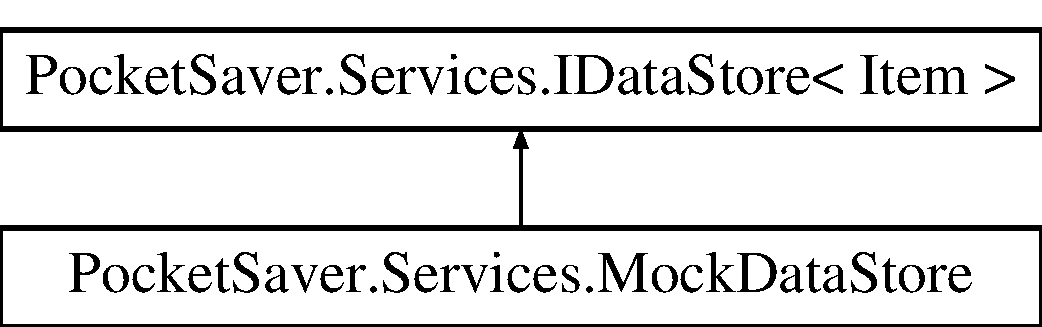
\includegraphics[height=2.000000cm]{class_pocket_saver_1_1_services_1_1_mock_data_store}
\end{center}
\end{figure}
\subsection*{Public Member Functions}
\begin{DoxyCompactItemize}
\item 
\mbox{\Hypertarget{class_pocket_saver_1_1_services_1_1_mock_data_store_a7d4b90a0525f662b848d4422bcaefebe}\label{class_pocket_saver_1_1_services_1_1_mock_data_store_a7d4b90a0525f662b848d4422bcaefebe}} 
async Task$<$ bool $>$ {\bfseries Add\+Item\+Async} (\hyperlink{class_pocket_saver_1_1_models_1_1_item}{Item} item)
\item 
\mbox{\Hypertarget{class_pocket_saver_1_1_services_1_1_mock_data_store_aadbfa26922ac219215a944975152190e}\label{class_pocket_saver_1_1_services_1_1_mock_data_store_aadbfa26922ac219215a944975152190e}} 
async Task$<$ bool $>$ {\bfseries Update\+Item\+Async} (\hyperlink{class_pocket_saver_1_1_models_1_1_item}{Item} item)
\item 
\mbox{\Hypertarget{class_pocket_saver_1_1_services_1_1_mock_data_store_ab0c404abbd057446da4095dc4e4abc12}\label{class_pocket_saver_1_1_services_1_1_mock_data_store_ab0c404abbd057446da4095dc4e4abc12}} 
async Task$<$ bool $>$ {\bfseries Delete\+Item\+Async} (\hyperlink{class_pocket_saver_1_1_models_1_1_item}{Item} item)
\item 
\mbox{\Hypertarget{class_pocket_saver_1_1_services_1_1_mock_data_store_ae68f480735063a93fbf5507da853077b}\label{class_pocket_saver_1_1_services_1_1_mock_data_store_ae68f480735063a93fbf5507da853077b}} 
async Task$<$ \hyperlink{class_pocket_saver_1_1_models_1_1_item}{Item} $>$ {\bfseries Get\+Item\+Async} (string id)
\item 
\mbox{\Hypertarget{class_pocket_saver_1_1_services_1_1_mock_data_store_a3a8300821f4859edbb51b01652183646}\label{class_pocket_saver_1_1_services_1_1_mock_data_store_a3a8300821f4859edbb51b01652183646}} 
async Task$<$ I\+Enumerable$<$ \hyperlink{class_pocket_saver_1_1_models_1_1_item}{Item} $>$ $>$ {\bfseries Get\+Items\+Async} (bool force\+Refresh=false)
\item 
\mbox{\Hypertarget{class_pocket_saver_1_1_services_1_1_mock_data_store_ac639240fa454cbdd00db0db7f01fe136}\label{class_pocket_saver_1_1_services_1_1_mock_data_store_ac639240fa454cbdd00db0db7f01fe136}} 
Task$<$ bool $>$ {\bfseries Pull\+Latest\+Async} ()
\item 
\mbox{\Hypertarget{class_pocket_saver_1_1_services_1_1_mock_data_store_a5a44b3150c7308915990c5411f3afbfe}\label{class_pocket_saver_1_1_services_1_1_mock_data_store_a5a44b3150c7308915990c5411f3afbfe}} 
Task$<$ bool $>$ {\bfseries Sync\+Async} ()
\item 
\mbox{\Hypertarget{class_pocket_saver_1_1_services_1_1_mock_data_store_aebef6f70f2548f3e703abfb65f46f16e}\label{class_pocket_saver_1_1_services_1_1_mock_data_store_aebef6f70f2548f3e703abfb65f46f16e}} 
async Task {\bfseries Initialize\+Async} ()
\end{DoxyCompactItemize}


The documentation for this class was generated from the following file\+:\begin{DoxyCompactItemize}
\item 
C\+:/\+Users/\+Mevin/\+Pocket\+Saver/src/\+Pocket\+Saver/\+Pocket\+Saver/\+Pocket\+Saver/\+Services/Mock\+Data\+Store.\+cs\end{DoxyCompactItemize}

\hypertarget{class_pocket_saver_1_1_helpers_1_1_negate_boolean_converter}{}\section{Pocket\+Saver.\+Helpers.\+Negate\+Boolean\+Converter Class Reference}
\label{class_pocket_saver_1_1_helpers_1_1_negate_boolean_converter}\index{Pocket\+Saver.\+Helpers.\+Negate\+Boolean\+Converter@{Pocket\+Saver.\+Helpers.\+Negate\+Boolean\+Converter}}


Class to create a converter for the X\+A\+ML values.  


Inheritance diagram for Pocket\+Saver.\+Helpers.\+Negate\+Boolean\+Converter\+:\begin{figure}[H]
\begin{center}
\leavevmode
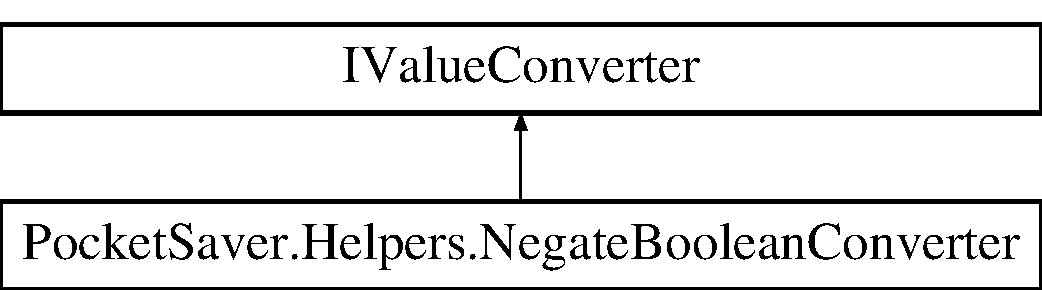
\includegraphics[height=2.000000cm]{class_pocket_saver_1_1_helpers_1_1_negate_boolean_converter}
\end{center}
\end{figure}
\subsection*{Public Member Functions}
\begin{DoxyCompactItemize}
\item 
\mbox{\Hypertarget{class_pocket_saver_1_1_helpers_1_1_negate_boolean_converter_a210dbb511fcb526fb0ebbea3f5f95e44}\label{class_pocket_saver_1_1_helpers_1_1_negate_boolean_converter_a210dbb511fcb526fb0ebbea3f5f95e44}} 
object {\bfseries Convert} (object value, Type target\+Type, object parameter, System.\+Globalization.\+Culture\+Info culture)
\item 
\mbox{\Hypertarget{class_pocket_saver_1_1_helpers_1_1_negate_boolean_converter_a2e798fe3f3ac99af7e00e7b3a8f52cd7}\label{class_pocket_saver_1_1_helpers_1_1_negate_boolean_converter_a2e798fe3f3ac99af7e00e7b3a8f52cd7}} 
object {\bfseries Convert\+Back} (object value, Type target\+Type, object parameter, System.\+Globalization.\+Culture\+Info culture)
\end{DoxyCompactItemize}


\subsection{Detailed Description}
Class to create a converter for the X\+A\+ML values. 



The documentation for this class was generated from the following file\+:\begin{DoxyCompactItemize}
\item 
C\+:/\+Users/\+Mevin/\+Pocket\+Saver/src/\+Pocket\+Saver/\+Pocket\+Saver/\+Pocket\+Saver/\+Helpers/Negate\+Boolean\+Converter.\+cs\end{DoxyCompactItemize}

\hypertarget{class_pocket_saver_1_1_views_1_1_new_item_page}{}\section{Pocket\+Saver.\+Views.\+New\+Item\+Page Class Reference}
\label{class_pocket_saver_1_1_views_1_1_new_item_page}\index{Pocket\+Saver.\+Views.\+New\+Item\+Page@{Pocket\+Saver.\+Views.\+New\+Item\+Page}}
Inheritance diagram for Pocket\+Saver.\+Views.\+New\+Item\+Page\+:\begin{figure}[H]
\begin{center}
\leavevmode
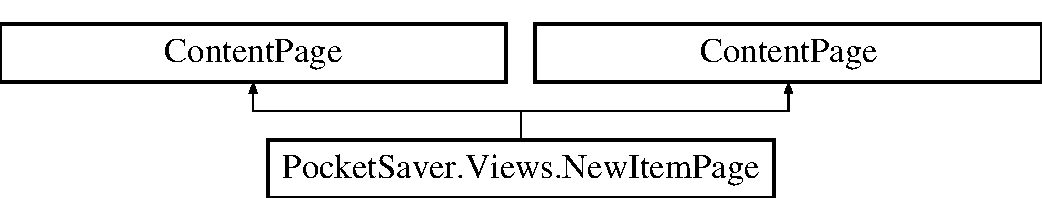
\includegraphics[height=2.000000cm]{class_pocket_saver_1_1_views_1_1_new_item_page}
\end{center}
\end{figure}
\subsection*{Properties}
\begin{DoxyCompactItemize}
\item 
\mbox{\Hypertarget{class_pocket_saver_1_1_views_1_1_new_item_page_abf4c99ff2acad5cfc5ac036ad0af2849}\label{class_pocket_saver_1_1_views_1_1_new_item_page_abf4c99ff2acad5cfc5ac036ad0af2849}} 
\hyperlink{class_pocket_saver_1_1_models_1_1_item}{Item} {\bfseries Item}\hspace{0.3cm}{\ttfamily  \mbox{[}get, set\mbox{]}}
\end{DoxyCompactItemize}


The documentation for this class was generated from the following files\+:\begin{DoxyCompactItemize}
\item 
C\+:/\+Users/\+Mevin/\+Pocket\+Saver/src/\+Pocket\+Saver/\+Pocket\+Saver/\+Pocket\+Saver/obj/\+Debug/Pocket\+Saver.\+Views.\+New\+Item\+Page.\+xaml.\+g.\+cs\item 
C\+:/\+Users/\+Mevin/\+Pocket\+Saver/src/\+Pocket\+Saver/\+Pocket\+Saver/\+Pocket\+Saver/\+Views/New\+Item\+Page.\+xaml.\+cs\end{DoxyCompactItemize}

\hypertarget{class_pocket_saver_1_1_helpers_1_1_observable_object}{}\section{Pocket\+Saver.\+Helpers.\+Observable\+Object Class Reference}
\label{class_pocket_saver_1_1_helpers_1_1_observable_object}\index{Pocket\+Saver.\+Helpers.\+Observable\+Object@{Pocket\+Saver.\+Helpers.\+Observable\+Object}}


Observable object with I\+Notify\+Property\+Changed implemented  


Inheritance diagram for Pocket\+Saver.\+Helpers.\+Observable\+Object\+:\begin{figure}[H]
\begin{center}
\leavevmode
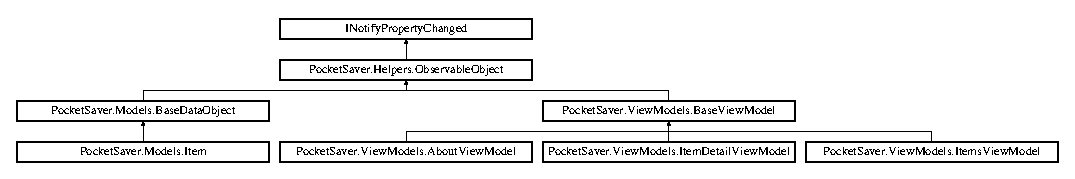
\includegraphics[height=1.958042cm]{class_pocket_saver_1_1_helpers_1_1_observable_object}
\end{center}
\end{figure}
\subsection*{Protected Member Functions}
\begin{DoxyCompactItemize}
\item 
bool \hyperlink{class_pocket_saver_1_1_helpers_1_1_observable_object_a0145f769ef5ed27c8031a768a0f9f53f}{Set\+Property$<$ T $>$} (ref T backing\+Store, T value, \mbox{[}Caller\+Member\+Name\mbox{]}string property\+Name=\char`\"{}\char`\"{}, Action on\+Changed=null)
\begin{DoxyCompactList}\small\item\em Sets the property. \end{DoxyCompactList}\item 
void \hyperlink{class_pocket_saver_1_1_helpers_1_1_observable_object_a3abc90b0599e021e2fd979a0cbff889c}{On\+Property\+Changed} (\mbox{[}Caller\+Member\+Name\mbox{]}string property\+Name=\char`\"{}\char`\"{})
\begin{DoxyCompactList}\small\item\em Raises the property changed event. \end{DoxyCompactList}\end{DoxyCompactItemize}
\subsection*{Events}
\begin{DoxyCompactItemize}
\item 
Property\+Changed\+Event\+Handler \hyperlink{class_pocket_saver_1_1_helpers_1_1_observable_object_a5bec60ddca9a88a38affe84844c2f16d}{Property\+Changed}
\begin{DoxyCompactList}\small\item\em Occurs when property changed. \end{DoxyCompactList}\end{DoxyCompactItemize}


\subsection{Detailed Description}
Observable object with I\+Notify\+Property\+Changed implemented 



\subsection{Member Function Documentation}
\mbox{\Hypertarget{class_pocket_saver_1_1_helpers_1_1_observable_object_a3abc90b0599e021e2fd979a0cbff889c}\label{class_pocket_saver_1_1_helpers_1_1_observable_object_a3abc90b0599e021e2fd979a0cbff889c}} 
\index{Pocket\+Saver\+::\+Helpers\+::\+Observable\+Object@{Pocket\+Saver\+::\+Helpers\+::\+Observable\+Object}!On\+Property\+Changed@{On\+Property\+Changed}}
\index{On\+Property\+Changed@{On\+Property\+Changed}!Pocket\+Saver\+::\+Helpers\+::\+Observable\+Object@{Pocket\+Saver\+::\+Helpers\+::\+Observable\+Object}}
\subsubsection{\texorpdfstring{On\+Property\+Changed()}{OnPropertyChanged()}}
{\footnotesize\ttfamily void Pocket\+Saver.\+Helpers.\+Observable\+Object.\+On\+Property\+Changed (\begin{DoxyParamCaption}\item[{\mbox{[}\+Caller\+Member\+Name\mbox{]} string}]{property\+Name = {\ttfamily \char`\"{}\char`\"{}} }\end{DoxyParamCaption})\hspace{0.3cm}{\ttfamily [inline]}, {\ttfamily [protected]}}



Raises the property changed event. 


\begin{DoxyParams}{Parameters}
{\em property\+Name} & Property name.\\
\hline
\end{DoxyParams}
\mbox{\Hypertarget{class_pocket_saver_1_1_helpers_1_1_observable_object_a0145f769ef5ed27c8031a768a0f9f53f}\label{class_pocket_saver_1_1_helpers_1_1_observable_object_a0145f769ef5ed27c8031a768a0f9f53f}} 
\index{Pocket\+Saver\+::\+Helpers\+::\+Observable\+Object@{Pocket\+Saver\+::\+Helpers\+::\+Observable\+Object}!Set\+Property$<$ T $>$@{Set\+Property$<$ T $>$}}
\index{Set\+Property$<$ T $>$@{Set\+Property$<$ T $>$}!Pocket\+Saver\+::\+Helpers\+::\+Observable\+Object@{Pocket\+Saver\+::\+Helpers\+::\+Observable\+Object}}
\subsubsection{\texorpdfstring{Set\+Property$<$ T $>$()}{SetProperty< T >()}}
{\footnotesize\ttfamily bool Pocket\+Saver.\+Helpers.\+Observable\+Object.\+Set\+Property$<$ T $>$ (\begin{DoxyParamCaption}\item[{ref T}]{backing\+Store,  }\item[{T}]{value,  }\item[{\mbox{[}\+Caller\+Member\+Name\mbox{]} string}]{property\+Name = {\ttfamily \char`\"{}\char`\"{}},  }\item[{Action}]{on\+Changed = {\ttfamily null} }\end{DoxyParamCaption})\hspace{0.3cm}{\ttfamily [inline]}, {\ttfamily [protected]}}



Sets the property. 

\begin{DoxyReturn}{Returns}
{\ttfamily true}, if property was set, {\ttfamily false} otherwise.
\end{DoxyReturn}

\begin{DoxyParams}{Parameters}
{\em backing\+Store} & Backing store.\\
\hline
{\em value} & Value.\\
\hline
{\em property\+Name} & Property name.\\
\hline
{\em on\+Changed} & On changed.\\
\hline
\end{DoxyParams}

\begin{DoxyTemplParams}{Template Parameters}
{\em T} & The 1st type parameter.\\
\hline
\end{DoxyTemplParams}


\subsection{Event Documentation}
\mbox{\Hypertarget{class_pocket_saver_1_1_helpers_1_1_observable_object_a5bec60ddca9a88a38affe84844c2f16d}\label{class_pocket_saver_1_1_helpers_1_1_observable_object_a5bec60ddca9a88a38affe84844c2f16d}} 
\index{Pocket\+Saver\+::\+Helpers\+::\+Observable\+Object@{Pocket\+Saver\+::\+Helpers\+::\+Observable\+Object}!Property\+Changed@{Property\+Changed}}
\index{Property\+Changed@{Property\+Changed}!Pocket\+Saver\+::\+Helpers\+::\+Observable\+Object@{Pocket\+Saver\+::\+Helpers\+::\+Observable\+Object}}
\subsubsection{\texorpdfstring{Property\+Changed}{PropertyChanged}}
{\footnotesize\ttfamily Property\+Changed\+Event\+Handler Pocket\+Saver.\+Helpers.\+Observable\+Object.\+Property\+Changed}



Occurs when property changed. 



The documentation for this class was generated from the following file\+:\begin{DoxyCompactItemize}
\item 
C\+:/\+Users/\+Mevin/\+Pocket\+Saver/src/\+Pocket\+Saver/\+Pocket\+Saver/\+Pocket\+Saver/\+Helpers/Observable\+Object.\+cs\end{DoxyCompactItemize}

\hypertarget{class_pocket_saver_1_1_helpers_1_1_observable_range_collection}{}\section{Pocket\+Saver.\+Helpers.\+Observable\+Range\+Collection$<$ T $>$ Class Template Reference}
\label{class_pocket_saver_1_1_helpers_1_1_observable_range_collection}\index{Pocket\+Saver.\+Helpers.\+Observable\+Range\+Collection$<$ T $>$@{Pocket\+Saver.\+Helpers.\+Observable\+Range\+Collection$<$ T $>$}}


Represents a dynamic data collection that provides notifications when items get added, removed, or when the whole list is refreshed.  


Inheritance diagram for Pocket\+Saver.\+Helpers.\+Observable\+Range\+Collection$<$ T $>$\+:\begin{figure}[H]
\begin{center}
\leavevmode
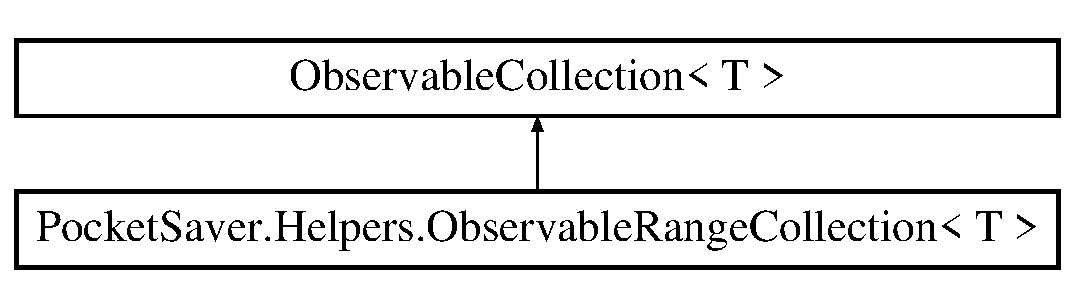
\includegraphics[height=2.000000cm]{class_pocket_saver_1_1_helpers_1_1_observable_range_collection}
\end{center}
\end{figure}
\subsection*{Public Member Functions}
\begin{DoxyCompactItemize}
\item 
\hyperlink{class_pocket_saver_1_1_helpers_1_1_observable_range_collection_a4d5992476c0c7143f8494dac1ab67b62}{Observable\+Range\+Collection} ()
\begin{DoxyCompactList}\small\item\em Initializes a new instance of the System.\+Collections.\+Object\+Model.\+Observable\+Collection(\+Of T) class. \end{DoxyCompactList}\item 
\hyperlink{class_pocket_saver_1_1_helpers_1_1_observable_range_collection_a20abe6e4757c17478a850e16bf32c28c}{Observable\+Range\+Collection} (I\+Enumerable$<$ T $>$ collection)
\begin{DoxyCompactList}\small\item\em Initializes a new instance of the System.\+Collections.\+Object\+Model.\+Observable\+Collection(\+Of T) class that contains elements copied from the specified collection. \end{DoxyCompactList}\item 
void \hyperlink{class_pocket_saver_1_1_helpers_1_1_observable_range_collection_ae9693a07699c4573faa9bca6bc291de2}{Add\+Range} (I\+Enumerable$<$ T $>$ collection, Notify\+Collection\+Changed\+Action notification\+Mode=Notify\+Collection\+Changed\+Action.\+Add)
\begin{DoxyCompactList}\small\item\em Adds the elements of the specified collection to the end of the Observable\+Collection(\+Of T). \end{DoxyCompactList}\item 
void \hyperlink{class_pocket_saver_1_1_helpers_1_1_observable_range_collection_a3d2e4bb0b0fb26b3dde6b1419cf46daa}{Remove\+Range} (I\+Enumerable$<$ T $>$ collection)
\begin{DoxyCompactList}\small\item\em Removes the first occurence of each item in the specified collection from Observable\+Collection(\+Of T). \end{DoxyCompactList}\item 
void \hyperlink{class_pocket_saver_1_1_helpers_1_1_observable_range_collection_a238e1f431d4b2ee17a29b51b0a4b0dc8}{Replace} (T item)
\begin{DoxyCompactList}\small\item\em Clears the current collection and replaces it with the specified item. \end{DoxyCompactList}\item 
void \hyperlink{class_pocket_saver_1_1_helpers_1_1_observable_range_collection_ac324fbc1de2bad4abe3c31252e94277f}{Replace\+Range} (I\+Enumerable$<$ T $>$ collection)
\begin{DoxyCompactList}\small\item\em Clears the current collection and replaces it with the specified collection. \end{DoxyCompactList}\end{DoxyCompactItemize}


\subsection{Detailed Description}
Represents a dynamic data collection that provides notifications when items get added, removed, or when the whole list is refreshed. 


\begin{DoxyTemplParams}{Template Parameters}
{\em T} & \\
\hline
\end{DoxyTemplParams}


\subsection{Constructor \& Destructor Documentation}
\mbox{\Hypertarget{class_pocket_saver_1_1_helpers_1_1_observable_range_collection_a4d5992476c0c7143f8494dac1ab67b62}\label{class_pocket_saver_1_1_helpers_1_1_observable_range_collection_a4d5992476c0c7143f8494dac1ab67b62}} 
\index{Pocket\+Saver\+::\+Helpers\+::\+Observable\+Range\+Collection@{Pocket\+Saver\+::\+Helpers\+::\+Observable\+Range\+Collection}!Observable\+Range\+Collection@{Observable\+Range\+Collection}}
\index{Observable\+Range\+Collection@{Observable\+Range\+Collection}!Pocket\+Saver\+::\+Helpers\+::\+Observable\+Range\+Collection@{Pocket\+Saver\+::\+Helpers\+::\+Observable\+Range\+Collection}}
\subsubsection{\texorpdfstring{Observable\+Range\+Collection()}{ObservableRangeCollection()}\hspace{0.1cm}{\footnotesize\ttfamily [1/2]}}
{\footnotesize\ttfamily \hyperlink{class_pocket_saver_1_1_helpers_1_1_observable_range_collection}{Pocket\+Saver.\+Helpers.\+Observable\+Range\+Collection}$<$ T $>$.\hyperlink{class_pocket_saver_1_1_helpers_1_1_observable_range_collection}{Observable\+Range\+Collection} (\begin{DoxyParamCaption}{ }\end{DoxyParamCaption})\hspace{0.3cm}{\ttfamily [inline]}}



Initializes a new instance of the System.\+Collections.\+Object\+Model.\+Observable\+Collection(\+Of T) class. 

\mbox{\Hypertarget{class_pocket_saver_1_1_helpers_1_1_observable_range_collection_a20abe6e4757c17478a850e16bf32c28c}\label{class_pocket_saver_1_1_helpers_1_1_observable_range_collection_a20abe6e4757c17478a850e16bf32c28c}} 
\index{Pocket\+Saver\+::\+Helpers\+::\+Observable\+Range\+Collection@{Pocket\+Saver\+::\+Helpers\+::\+Observable\+Range\+Collection}!Observable\+Range\+Collection@{Observable\+Range\+Collection}}
\index{Observable\+Range\+Collection@{Observable\+Range\+Collection}!Pocket\+Saver\+::\+Helpers\+::\+Observable\+Range\+Collection@{Pocket\+Saver\+::\+Helpers\+::\+Observable\+Range\+Collection}}
\subsubsection{\texorpdfstring{Observable\+Range\+Collection()}{ObservableRangeCollection()}\hspace{0.1cm}{\footnotesize\ttfamily [2/2]}}
{\footnotesize\ttfamily \hyperlink{class_pocket_saver_1_1_helpers_1_1_observable_range_collection}{Pocket\+Saver.\+Helpers.\+Observable\+Range\+Collection}$<$ T $>$.\hyperlink{class_pocket_saver_1_1_helpers_1_1_observable_range_collection}{Observable\+Range\+Collection} (\begin{DoxyParamCaption}\item[{I\+Enumerable$<$ T $>$}]{collection }\end{DoxyParamCaption})\hspace{0.3cm}{\ttfamily [inline]}}



Initializes a new instance of the System.\+Collections.\+Object\+Model.\+Observable\+Collection(\+Of T) class that contains elements copied from the specified collection. 


\begin{DoxyParams}{Parameters}
{\em collection} & collection\+: The collection from which the elements are copied.\\
\hline
\end{DoxyParams}

\begin{DoxyExceptions}{Exceptions}
{\em System.\+Argument\+Null\+Exception} & The collection parameter cannot be null.\\
\hline
\end{DoxyExceptions}


\subsection{Member Function Documentation}
\mbox{\Hypertarget{class_pocket_saver_1_1_helpers_1_1_observable_range_collection_ae9693a07699c4573faa9bca6bc291de2}\label{class_pocket_saver_1_1_helpers_1_1_observable_range_collection_ae9693a07699c4573faa9bca6bc291de2}} 
\index{Pocket\+Saver\+::\+Helpers\+::\+Observable\+Range\+Collection@{Pocket\+Saver\+::\+Helpers\+::\+Observable\+Range\+Collection}!Add\+Range@{Add\+Range}}
\index{Add\+Range@{Add\+Range}!Pocket\+Saver\+::\+Helpers\+::\+Observable\+Range\+Collection@{Pocket\+Saver\+::\+Helpers\+::\+Observable\+Range\+Collection}}
\subsubsection{\texorpdfstring{Add\+Range()}{AddRange()}}
{\footnotesize\ttfamily void \hyperlink{class_pocket_saver_1_1_helpers_1_1_observable_range_collection}{Pocket\+Saver.\+Helpers.\+Observable\+Range\+Collection}$<$ T $>$.Add\+Range (\begin{DoxyParamCaption}\item[{I\+Enumerable$<$ T $>$}]{collection,  }\item[{Notify\+Collection\+Changed\+Action}]{notification\+Mode = {\ttfamily NotifyCollectionChangedAction.Add} }\end{DoxyParamCaption})\hspace{0.3cm}{\ttfamily [inline]}}



Adds the elements of the specified collection to the end of the Observable\+Collection(\+Of T). 

\mbox{\Hypertarget{class_pocket_saver_1_1_helpers_1_1_observable_range_collection_a3d2e4bb0b0fb26b3dde6b1419cf46daa}\label{class_pocket_saver_1_1_helpers_1_1_observable_range_collection_a3d2e4bb0b0fb26b3dde6b1419cf46daa}} 
\index{Pocket\+Saver\+::\+Helpers\+::\+Observable\+Range\+Collection@{Pocket\+Saver\+::\+Helpers\+::\+Observable\+Range\+Collection}!Remove\+Range@{Remove\+Range}}
\index{Remove\+Range@{Remove\+Range}!Pocket\+Saver\+::\+Helpers\+::\+Observable\+Range\+Collection@{Pocket\+Saver\+::\+Helpers\+::\+Observable\+Range\+Collection}}
\subsubsection{\texorpdfstring{Remove\+Range()}{RemoveRange()}}
{\footnotesize\ttfamily void \hyperlink{class_pocket_saver_1_1_helpers_1_1_observable_range_collection}{Pocket\+Saver.\+Helpers.\+Observable\+Range\+Collection}$<$ T $>$.Remove\+Range (\begin{DoxyParamCaption}\item[{I\+Enumerable$<$ T $>$}]{collection }\end{DoxyParamCaption})\hspace{0.3cm}{\ttfamily [inline]}}



Removes the first occurence of each item in the specified collection from Observable\+Collection(\+Of T). 

\mbox{\Hypertarget{class_pocket_saver_1_1_helpers_1_1_observable_range_collection_a238e1f431d4b2ee17a29b51b0a4b0dc8}\label{class_pocket_saver_1_1_helpers_1_1_observable_range_collection_a238e1f431d4b2ee17a29b51b0a4b0dc8}} 
\index{Pocket\+Saver\+::\+Helpers\+::\+Observable\+Range\+Collection@{Pocket\+Saver\+::\+Helpers\+::\+Observable\+Range\+Collection}!Replace@{Replace}}
\index{Replace@{Replace}!Pocket\+Saver\+::\+Helpers\+::\+Observable\+Range\+Collection@{Pocket\+Saver\+::\+Helpers\+::\+Observable\+Range\+Collection}}
\subsubsection{\texorpdfstring{Replace()}{Replace()}}
{\footnotesize\ttfamily void \hyperlink{class_pocket_saver_1_1_helpers_1_1_observable_range_collection}{Pocket\+Saver.\+Helpers.\+Observable\+Range\+Collection}$<$ T $>$.Replace (\begin{DoxyParamCaption}\item[{T}]{item }\end{DoxyParamCaption})\hspace{0.3cm}{\ttfamily [inline]}}



Clears the current collection and replaces it with the specified item. 

\mbox{\Hypertarget{class_pocket_saver_1_1_helpers_1_1_observable_range_collection_ac324fbc1de2bad4abe3c31252e94277f}\label{class_pocket_saver_1_1_helpers_1_1_observable_range_collection_ac324fbc1de2bad4abe3c31252e94277f}} 
\index{Pocket\+Saver\+::\+Helpers\+::\+Observable\+Range\+Collection@{Pocket\+Saver\+::\+Helpers\+::\+Observable\+Range\+Collection}!Replace\+Range@{Replace\+Range}}
\index{Replace\+Range@{Replace\+Range}!Pocket\+Saver\+::\+Helpers\+::\+Observable\+Range\+Collection@{Pocket\+Saver\+::\+Helpers\+::\+Observable\+Range\+Collection}}
\subsubsection{\texorpdfstring{Replace\+Range()}{ReplaceRange()}}
{\footnotesize\ttfamily void \hyperlink{class_pocket_saver_1_1_helpers_1_1_observable_range_collection}{Pocket\+Saver.\+Helpers.\+Observable\+Range\+Collection}$<$ T $>$.Replace\+Range (\begin{DoxyParamCaption}\item[{I\+Enumerable$<$ T $>$}]{collection }\end{DoxyParamCaption})\hspace{0.3cm}{\ttfamily [inline]}}



Clears the current collection and replaces it with the specified collection. 



The documentation for this class was generated from the following file\+:\begin{DoxyCompactItemize}
\item 
C\+:/\+Users/\+Mevin/\+Pocket\+Saver/src/\+Pocket\+Saver/\+Pocket\+Saver/\+Pocket\+Saver/\+Helpers/Observable\+Range\+Collection.\+cs\end{DoxyCompactItemize}

\hypertarget{class_pocket_saver_1_1_views_1_1_shared_1_1_page_activity_indicator}{}\section{Pocket\+Saver.\+Views.\+Shared.\+Page\+Activity\+Indicator Class Reference}
\label{class_pocket_saver_1_1_views_1_1_shared_1_1_page_activity_indicator}\index{Pocket\+Saver.\+Views.\+Shared.\+Page\+Activity\+Indicator@{Pocket\+Saver.\+Views.\+Shared.\+Page\+Activity\+Indicator}}


Class for the \hyperlink{class_pocket_saver_1_1_views_1_1_shared_1_1_page_activity_indicator}{Page\+Activity\+Indicator}.  


Inheritance diagram for Pocket\+Saver.\+Views.\+Shared.\+Page\+Activity\+Indicator\+:\begin{figure}[H]
\begin{center}
\leavevmode
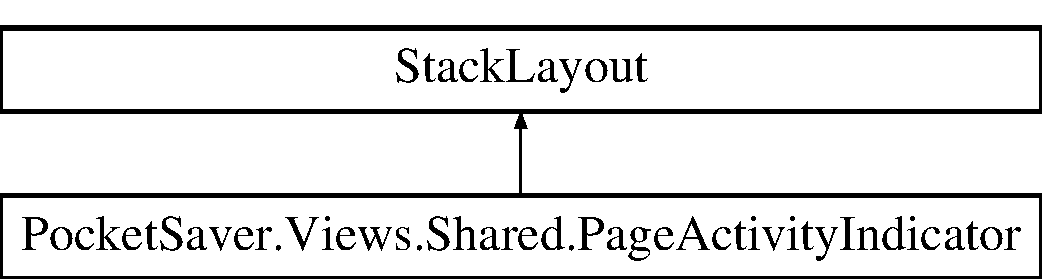
\includegraphics[height=2.000000cm]{class_pocket_saver_1_1_views_1_1_shared_1_1_page_activity_indicator}
\end{center}
\end{figure}
\subsection*{Public Member Functions}
\begin{DoxyCompactItemize}
\item 
\mbox{\Hypertarget{class_pocket_saver_1_1_views_1_1_shared_1_1_page_activity_indicator_a11a3ee43d93c39e168dde85c60ee02ce}\label{class_pocket_saver_1_1_views_1_1_shared_1_1_page_activity_indicator_a11a3ee43d93c39e168dde85c60ee02ce}} 
async Task {\bfseries Begin} ()
\item 
\mbox{\Hypertarget{class_pocket_saver_1_1_views_1_1_shared_1_1_page_activity_indicator_a508cd9e1cbd2984270f403249a986d8d}\label{class_pocket_saver_1_1_views_1_1_shared_1_1_page_activity_indicator_a508cd9e1cbd2984270f403249a986d8d}} 
async Task {\bfseries End} ()
\end{DoxyCompactItemize}
\subsection*{Public Attributes}
\begin{DoxyCompactItemize}
\item 
\mbox{\Hypertarget{class_pocket_saver_1_1_views_1_1_shared_1_1_page_activity_indicator_a36cdc07ae4b40eb9822603a03286272c}\label{class_pocket_saver_1_1_views_1_1_shared_1_1_page_activity_indicator_a36cdc07ae4b40eb9822603a03286272c}} 
bool {\bfseries Activated} = true
\end{DoxyCompactItemize}
\subsection*{Static Public Attributes}
\begin{DoxyCompactItemize}
\item 
static readonly Bindable\+Property {\bfseries Running\+Property}
\end{DoxyCompactItemize}
\subsection*{Properties}
\begin{DoxyCompactItemize}
\item 
\mbox{\Hypertarget{class_pocket_saver_1_1_views_1_1_shared_1_1_page_activity_indicator_a96fd76ee472796640439c1cadd3d0d92}\label{class_pocket_saver_1_1_views_1_1_shared_1_1_page_activity_indicator_a96fd76ee472796640439c1cadd3d0d92}} 
bool {\bfseries Running}\hspace{0.3cm}{\ttfamily  \mbox{[}get, set\mbox{]}}
\end{DoxyCompactItemize}


\subsection{Detailed Description}
Class for the \hyperlink{class_pocket_saver_1_1_views_1_1_shared_1_1_page_activity_indicator}{Page\+Activity\+Indicator}. 



\subsection{Member Data Documentation}
\mbox{\Hypertarget{class_pocket_saver_1_1_views_1_1_shared_1_1_page_activity_indicator_a86bdcba4778c1358d04628cbc90bf0b9}\label{class_pocket_saver_1_1_views_1_1_shared_1_1_page_activity_indicator_a86bdcba4778c1358d04628cbc90bf0b9}} 
\index{Pocket\+Saver\+::\+Views\+::\+Shared\+::\+Page\+Activity\+Indicator@{Pocket\+Saver\+::\+Views\+::\+Shared\+::\+Page\+Activity\+Indicator}!Running\+Property@{Running\+Property}}
\index{Running\+Property@{Running\+Property}!Pocket\+Saver\+::\+Views\+::\+Shared\+::\+Page\+Activity\+Indicator@{Pocket\+Saver\+::\+Views\+::\+Shared\+::\+Page\+Activity\+Indicator}}
\subsubsection{\texorpdfstring{Running\+Property}{RunningProperty}}
{\footnotesize\ttfamily readonly Bindable\+Property Pocket\+Saver.\+Views.\+Shared.\+Page\+Activity\+Indicator.\+Running\+Property\hspace{0.3cm}{\ttfamily [static]}}

{\bfseries Initial value\+:}
\begin{DoxyCode}
= BindableProperty.Create(
            propertyName: \textcolor{stringliteral}{"Running"},
            returnType: typeof(\textcolor{keywordtype}{bool}),
            declaringType: typeof(PageActivityIndicator),
            defaultValue: \textcolor{keyword}{true},
            propertyChanged: RunningChanged)
\end{DoxyCode}


The documentation for this class was generated from the following file\+:\begin{DoxyCompactItemize}
\item 
C\+:/\+Users/\+Mevin/\+Pocket\+Saver/src/\+Pocket\+Saver/\+Pocket\+Saver/\+Pocket\+Saver/\+Views/\+Shared/Page\+Activity\+Indicator.\+cs\end{DoxyCompactItemize}

\hypertarget{class_pocket_saver_1_1_views_1_1_settings_1_1_settings_page}{}\section{Pocket\+Saver.\+Views.\+Settings.\+Settings\+Page Class Reference}
\label{class_pocket_saver_1_1_views_1_1_settings_1_1_settings_page}\index{Pocket\+Saver.\+Views.\+Settings.\+Settings\+Page@{Pocket\+Saver.\+Views.\+Settings.\+Settings\+Page}}


Class for the \hyperlink{class_pocket_saver_1_1_views_1_1_settings_1_1_settings_page}{Settings\+Page} View.  


Inheritance diagram for Pocket\+Saver.\+Views.\+Settings.\+Settings\+Page\+:\begin{figure}[H]
\begin{center}
\leavevmode
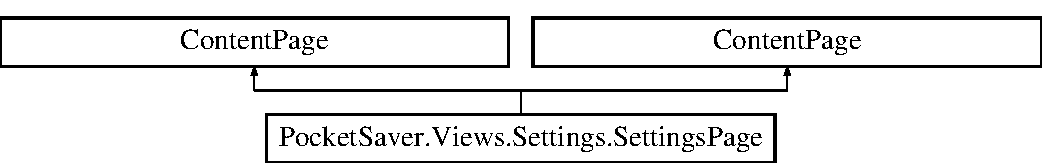
\includegraphics[height=1.464052cm]{class_pocket_saver_1_1_views_1_1_settings_1_1_settings_page}
\end{center}
\end{figure}
\subsection*{Public Member Functions}
\begin{DoxyCompactItemize}
\item 
\hyperlink{class_pocket_saver_1_1_views_1_1_settings_1_1_settings_page_a14d3be3fc03e6f84aaa08ee172bd3c3a}{Settings\+Page} ()
\begin{DoxyCompactList}\small\item\em Constructor for the \hyperlink{class_pocket_saver_1_1_views_1_1_settings_1_1_settings_page}{Settings\+Page}. \end{DoxyCompactList}\end{DoxyCompactItemize}


\subsection{Detailed Description}
Class for the \hyperlink{class_pocket_saver_1_1_views_1_1_settings_1_1_settings_page}{Settings\+Page} View. 



\subsection{Constructor \& Destructor Documentation}
\mbox{\Hypertarget{class_pocket_saver_1_1_views_1_1_settings_1_1_settings_page_a14d3be3fc03e6f84aaa08ee172bd3c3a}\label{class_pocket_saver_1_1_views_1_1_settings_1_1_settings_page_a14d3be3fc03e6f84aaa08ee172bd3c3a}} 
\index{Pocket\+Saver\+::\+Views\+::\+Settings\+::\+Settings\+Page@{Pocket\+Saver\+::\+Views\+::\+Settings\+::\+Settings\+Page}!Settings\+Page@{Settings\+Page}}
\index{Settings\+Page@{Settings\+Page}!Pocket\+Saver\+::\+Views\+::\+Settings\+::\+Settings\+Page@{Pocket\+Saver\+::\+Views\+::\+Settings\+::\+Settings\+Page}}
\subsubsection{\texorpdfstring{Settings\+Page()}{SettingsPage()}}
{\footnotesize\ttfamily Pocket\+Saver.\+Views.\+Settings.\+Settings\+Page.\+Settings\+Page (\begin{DoxyParamCaption}{ }\end{DoxyParamCaption})\hspace{0.3cm}{\ttfamily [inline]}}



Constructor for the \hyperlink{class_pocket_saver_1_1_views_1_1_settings_1_1_settings_page}{Settings\+Page}. 



The documentation for this class was generated from the following files\+:\begin{DoxyCompactItemize}
\item 
C\+:/\+Users/\+Mevin/\+Pocket\+Saver/src/\+Pocket\+Saver/\+Pocket\+Saver/\+Pocket\+Saver/obj/\+Debug/Pocket\+Saver.\+Views.\+Settings.\+Settings\+Page.\+xaml.\+g.\+cs\item 
C\+:/\+Users/\+Mevin/\+Pocket\+Saver/src/\+Pocket\+Saver/\+Pocket\+Saver/\+Pocket\+Saver/obj/\+Debug/Pocket\+Saver.\+Views.\+Transaction.\+Settings.\+Settings\+Page.\+xaml.\+g.\+cs\item 
C\+:/\+Users/\+Mevin/\+Pocket\+Saver/src/\+Pocket\+Saver/\+Pocket\+Saver/\+Pocket\+Saver/\+Views/\+Settings/Settings\+Page.\+xaml.\+cs\end{DoxyCompactItemize}

\hypertarget{class_pocket_saver_1_1_views_1_1_shared_1_1_tinted_image}{}\section{Pocket\+Saver.\+Views.\+Shared.\+Tinted\+Image Class Reference}
\label{class_pocket_saver_1_1_views_1_1_shared_1_1_tinted_image}\index{Pocket\+Saver.\+Views.\+Shared.\+Tinted\+Image@{Pocket\+Saver.\+Views.\+Shared.\+Tinted\+Image}}


Class for the Tinted image.  


Inheritance diagram for Pocket\+Saver.\+Views.\+Shared.\+Tinted\+Image\+:\begin{figure}[H]
\begin{center}
\leavevmode
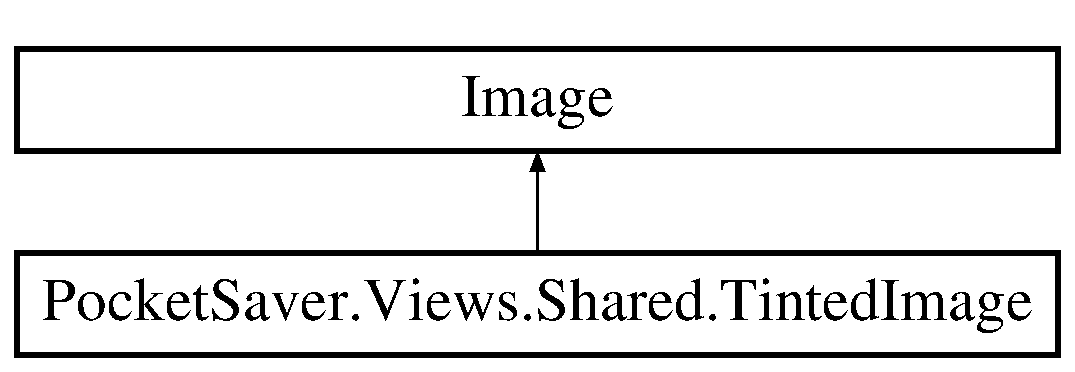
\includegraphics[height=2.000000cm]{class_pocket_saver_1_1_views_1_1_shared_1_1_tinted_image}
\end{center}
\end{figure}
\subsection*{Static Public Attributes}
\begin{DoxyCompactItemize}
\item 
\mbox{\Hypertarget{class_pocket_saver_1_1_views_1_1_shared_1_1_tinted_image_add1972fe38ceea5b39462e3e3b949e92}\label{class_pocket_saver_1_1_views_1_1_shared_1_1_tinted_image_add1972fe38ceea5b39462e3e3b949e92}} 
static readonly Bindable\+Property {\bfseries Tint\+Color\+Property} = Bindable\+Property.\+Create(nameof(Tint\+Color), typeof(Color), typeof(\hyperlink{class_pocket_saver_1_1_views_1_1_shared_1_1_tinted_image}{Tinted\+Image}), Color.\+Black)
\end{DoxyCompactItemize}
\subsection*{Properties}
\begin{DoxyCompactItemize}
\item 
\mbox{\Hypertarget{class_pocket_saver_1_1_views_1_1_shared_1_1_tinted_image_a00c93f802da9c98ed59805c8804c6d66}\label{class_pocket_saver_1_1_views_1_1_shared_1_1_tinted_image_a00c93f802da9c98ed59805c8804c6d66}} 
Color {\bfseries Tint\+Color}\hspace{0.3cm}{\ttfamily  \mbox{[}get, set\mbox{]}}
\end{DoxyCompactItemize}


\subsection{Detailed Description}
Class for the Tinted image. 



The documentation for this class was generated from the following file\+:\begin{DoxyCompactItemize}
\item 
C\+:/\+Users/\+Mevin/\+Pocket\+Saver/src/\+Pocket\+Saver/\+Pocket\+Saver/\+Pocket\+Saver/\+Views/\+Shared/Tinted\+Image.\+cs\end{DoxyCompactItemize}

\hypertarget{class_pocket_saver_1_1_views_1_1_transaction_1_1_transaction_detail}{}\section{Pocket\+Saver.\+Views.\+Transaction.\+Transaction\+Detail Class Reference}
\label{class_pocket_saver_1_1_views_1_1_transaction_1_1_transaction_detail}\index{Pocket\+Saver.\+Views.\+Transaction.\+Transaction\+Detail@{Pocket\+Saver.\+Views.\+Transaction.\+Transaction\+Detail}}


Class for the \hyperlink{class_pocket_saver_1_1_views_1_1_transaction_1_1_transaction_detail}{Transaction\+Detail} page for the \hyperlink{namespace_pocket_saver}{Pocket\+Saver} application.  


Inheritance diagram for Pocket\+Saver.\+Views.\+Transaction.\+Transaction\+Detail\+:\begin{figure}[H]
\begin{center}
\leavevmode
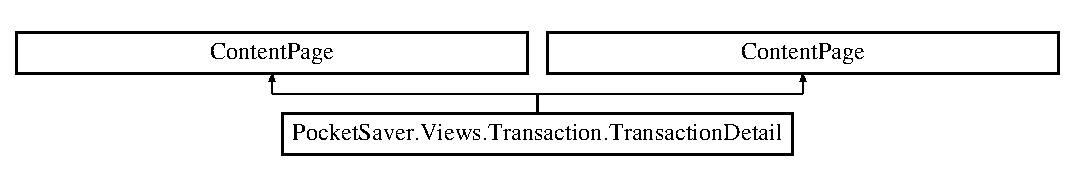
\includegraphics[height=1.854305cm]{class_pocket_saver_1_1_views_1_1_transaction_1_1_transaction_detail}
\end{center}
\end{figure}
\subsection*{Public Member Functions}
\begin{DoxyCompactItemize}
\item 
\hyperlink{class_pocket_saver_1_1_views_1_1_transaction_1_1_transaction_detail_a3071272e4982e10b355f107097023f90}{Transaction\+Detail} (String id, String category, String comment, Date\+Time date, Decimal purchase\+Amount)
\begin{DoxyCompactList}\small\item\em Constructor for the \hyperlink{class_pocket_saver_1_1_views_1_1_transaction_1_1_transaction_detail}{Transaction\+Detail} \end{DoxyCompactList}\end{DoxyCompactItemize}


\subsection{Detailed Description}
Class for the \hyperlink{class_pocket_saver_1_1_views_1_1_transaction_1_1_transaction_detail}{Transaction\+Detail} page for the \hyperlink{namespace_pocket_saver}{Pocket\+Saver} application. 



\subsection{Constructor \& Destructor Documentation}
\mbox{\Hypertarget{class_pocket_saver_1_1_views_1_1_transaction_1_1_transaction_detail_a3071272e4982e10b355f107097023f90}\label{class_pocket_saver_1_1_views_1_1_transaction_1_1_transaction_detail_a3071272e4982e10b355f107097023f90}} 
\index{Pocket\+Saver\+::\+Views\+::\+Transaction\+::\+Transaction\+Detail@{Pocket\+Saver\+::\+Views\+::\+Transaction\+::\+Transaction\+Detail}!Transaction\+Detail@{Transaction\+Detail}}
\index{Transaction\+Detail@{Transaction\+Detail}!Pocket\+Saver\+::\+Views\+::\+Transaction\+::\+Transaction\+Detail@{Pocket\+Saver\+::\+Views\+::\+Transaction\+::\+Transaction\+Detail}}
\subsubsection{\texorpdfstring{Transaction\+Detail()}{TransactionDetail()}}
{\footnotesize\ttfamily Pocket\+Saver.\+Views.\+Transaction.\+Transaction\+Detail.\+Transaction\+Detail (\begin{DoxyParamCaption}\item[{String}]{id,  }\item[{String}]{category,  }\item[{String}]{comment,  }\item[{Date\+Time}]{date,  }\item[{Decimal}]{purchase\+Amount }\end{DoxyParamCaption})\hspace{0.3cm}{\ttfamily [inline]}}



Constructor for the \hyperlink{class_pocket_saver_1_1_views_1_1_transaction_1_1_transaction_detail}{Transaction\+Detail} 


\begin{DoxyParams}{Parameters}
{\em id} & string id is the id retrieved from the database for the Transaction\+Model Object\\
\hline
{\em category} & string category is the category retrieved from the database for the Transaction\+Model Object\\
\hline
{\em comment} & string comment is the comment retrieved from the database for the Transaction\+Model Object\\
\hline
{\em date} & Date\+Time date is the date retrieved from the database for the Transaction\+Model Object\\
\hline
{\em purchase\+Amount} & Decimal purchase\+Amount is the purchase amount retrieved from the database for the Transaction\+Model Object\\
\hline
\end{DoxyParams}


The documentation for this class was generated from the following files\+:\begin{DoxyCompactItemize}
\item 
C\+:/\+Users/\+Mevin/\+Pocket\+Saver/src/\+Pocket\+Saver/\+Pocket\+Saver/\+Pocket\+Saver/obj/\+Debug/Pocket\+Saver.\+Views.\+Transaction.\+Transaction\+Detail.\+xaml.\+g.\+cs\item 
C\+:/\+Users/\+Mevin/\+Pocket\+Saver/src/\+Pocket\+Saver/\+Pocket\+Saver/\+Pocket\+Saver/\+Views/\+Transaction/Transaction\+Detail.\+xaml.\+cs\end{DoxyCompactItemize}

\hypertarget{class_pocket_saver_1_1_views_1_1_transaction_1_1_transaction_edit_page}{}\section{Pocket\+Saver.\+Views.\+Transaction.\+Transaction\+Edit\+Page Class Reference}
\label{class_pocket_saver_1_1_views_1_1_transaction_1_1_transaction_edit_page}\index{Pocket\+Saver.\+Views.\+Transaction.\+Transaction\+Edit\+Page@{Pocket\+Saver.\+Views.\+Transaction.\+Transaction\+Edit\+Page}}


Class for the \hyperlink{class_pocket_saver_1_1_views_1_1_transaction_1_1_transaction_edit_page}{Transaction\+Edit\+Page} for the \hyperlink{namespace_pocket_saver}{Pocket\+Saver} Mobile.  


Inheritance diagram for Pocket\+Saver.\+Views.\+Transaction.\+Transaction\+Edit\+Page\+:\begin{figure}[H]
\begin{center}
\leavevmode
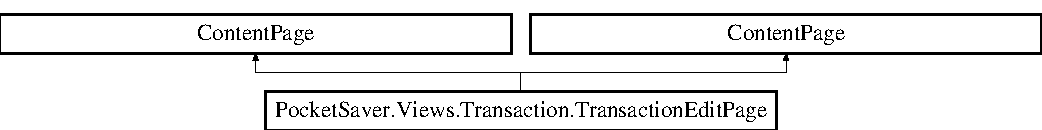
\includegraphics[height=1.750000cm]{class_pocket_saver_1_1_views_1_1_transaction_1_1_transaction_edit_page}
\end{center}
\end{figure}
\subsection*{Public Member Functions}
\begin{DoxyCompactItemize}
\item 
\hyperlink{class_pocket_saver_1_1_views_1_1_transaction_1_1_transaction_edit_page_a6e4aa411cc567c67418fdc425e574551}{Transaction\+Edit\+Page} ()
\begin{DoxyCompactList}\small\item\em Constructor for the \hyperlink{class_pocket_saver_1_1_views_1_1_transaction_1_1_transaction_edit_page}{Transaction\+Edit\+Page} \end{DoxyCompactList}\item 
\hyperlink{class_pocket_saver_1_1_views_1_1_transaction_1_1_transaction_edit_page_a919496a1e0b09b26162d89918b2fe9f6}{Transaction\+Edit\+Page} (string t\+Id, string category, string comment, Date\+Time date, Decimal purchase\+Amount)
\begin{DoxyCompactList}\small\item\em Constructor overload for the \hyperlink{class_pocket_saver_1_1_views_1_1_transaction_1_1_transaction_edit_page}{Transaction\+Edit\+Page}. \end{DoxyCompactList}\end{DoxyCompactItemize}


\subsection{Detailed Description}
Class for the \hyperlink{class_pocket_saver_1_1_views_1_1_transaction_1_1_transaction_edit_page}{Transaction\+Edit\+Page} for the \hyperlink{namespace_pocket_saver}{Pocket\+Saver} Mobile. 



\subsection{Constructor \& Destructor Documentation}
\mbox{\Hypertarget{class_pocket_saver_1_1_views_1_1_transaction_1_1_transaction_edit_page_a6e4aa411cc567c67418fdc425e574551}\label{class_pocket_saver_1_1_views_1_1_transaction_1_1_transaction_edit_page_a6e4aa411cc567c67418fdc425e574551}} 
\index{Pocket\+Saver\+::\+Views\+::\+Transaction\+::\+Transaction\+Edit\+Page@{Pocket\+Saver\+::\+Views\+::\+Transaction\+::\+Transaction\+Edit\+Page}!Transaction\+Edit\+Page@{Transaction\+Edit\+Page}}
\index{Transaction\+Edit\+Page@{Transaction\+Edit\+Page}!Pocket\+Saver\+::\+Views\+::\+Transaction\+::\+Transaction\+Edit\+Page@{Pocket\+Saver\+::\+Views\+::\+Transaction\+::\+Transaction\+Edit\+Page}}
\subsubsection{\texorpdfstring{Transaction\+Edit\+Page()}{TransactionEditPage()}\hspace{0.1cm}{\footnotesize\ttfamily [1/2]}}
{\footnotesize\ttfamily Pocket\+Saver.\+Views.\+Transaction.\+Transaction\+Edit\+Page.\+Transaction\+Edit\+Page (\begin{DoxyParamCaption}{ }\end{DoxyParamCaption})\hspace{0.3cm}{\ttfamily [inline]}}



Constructor for the \hyperlink{class_pocket_saver_1_1_views_1_1_transaction_1_1_transaction_edit_page}{Transaction\+Edit\+Page} 

\mbox{\Hypertarget{class_pocket_saver_1_1_views_1_1_transaction_1_1_transaction_edit_page_a919496a1e0b09b26162d89918b2fe9f6}\label{class_pocket_saver_1_1_views_1_1_transaction_1_1_transaction_edit_page_a919496a1e0b09b26162d89918b2fe9f6}} 
\index{Pocket\+Saver\+::\+Views\+::\+Transaction\+::\+Transaction\+Edit\+Page@{Pocket\+Saver\+::\+Views\+::\+Transaction\+::\+Transaction\+Edit\+Page}!Transaction\+Edit\+Page@{Transaction\+Edit\+Page}}
\index{Transaction\+Edit\+Page@{Transaction\+Edit\+Page}!Pocket\+Saver\+::\+Views\+::\+Transaction\+::\+Transaction\+Edit\+Page@{Pocket\+Saver\+::\+Views\+::\+Transaction\+::\+Transaction\+Edit\+Page}}
\subsubsection{\texorpdfstring{Transaction\+Edit\+Page()}{TransactionEditPage()}\hspace{0.1cm}{\footnotesize\ttfamily [2/2]}}
{\footnotesize\ttfamily Pocket\+Saver.\+Views.\+Transaction.\+Transaction\+Edit\+Page.\+Transaction\+Edit\+Page (\begin{DoxyParamCaption}\item[{string}]{t\+Id,  }\item[{string}]{category,  }\item[{string}]{comment,  }\item[{Date\+Time}]{date,  }\item[{Decimal}]{purchase\+Amount }\end{DoxyParamCaption})\hspace{0.3cm}{\ttfamily [inline]}}



Constructor overload for the \hyperlink{class_pocket_saver_1_1_views_1_1_transaction_1_1_transaction_edit_page}{Transaction\+Edit\+Page}. 


\begin{DoxyParams}{Parameters}
{\em t\+Id} & string t\+Id is the id retrieved from the database for the Transaction\+Model Object\\
\hline
{\em category} & string category is the category retrieved from the database for the Transaction\+Model Object\\
\hline
{\em comment} & string comment is the comment retrieved from the database for the Transaction\+Model Object\\
\hline
{\em date} & Date\+Time date is the date retrieved from the database for the Transaction\+Model Object\\
\hline
{\em purchase\+Amount} & Decimal purchase\+Amount is the purchase amount retrieved from the database for the Transaction\+Model Object\\
\hline
\end{DoxyParams}


The documentation for this class was generated from the following files\+:\begin{DoxyCompactItemize}
\item 
C\+:/\+Users/\+Mevin/\+Pocket\+Saver/src/\+Pocket\+Saver/\+Pocket\+Saver/\+Pocket\+Saver/obj/\+Debug/Pocket\+Saver.\+Views.\+Transaction.\+Transaction\+Edit\+Page.\+xaml.\+g.\+cs\item 
C\+:/\+Users/\+Mevin/\+Pocket\+Saver/src/\+Pocket\+Saver/\+Pocket\+Saver/\+Pocket\+Saver/\+Views/\+Transaction/Transaction\+Edit\+Page.\+xaml.\+cs\end{DoxyCompactItemize}

\hypertarget{class_pocket_saver_1_1_views_1_1_transaction_1_1_transaction_list_cell}{}\section{Pocket\+Saver.\+Views.\+Transaction.\+Transaction\+List\+Cell Class Reference}
\label{class_pocket_saver_1_1_views_1_1_transaction_1_1_transaction_list_cell}\index{Pocket\+Saver.\+Views.\+Transaction.\+Transaction\+List\+Cell@{Pocket\+Saver.\+Views.\+Transaction.\+Transaction\+List\+Cell}}


Class for the \hyperlink{class_pocket_saver_1_1_views_1_1_transaction_1_1_transaction_list_cell}{Transaction\+List\+Cell}  


Inheritance diagram for Pocket\+Saver.\+Views.\+Transaction.\+Transaction\+List\+Cell\+:\begin{figure}[H]
\begin{center}
\leavevmode
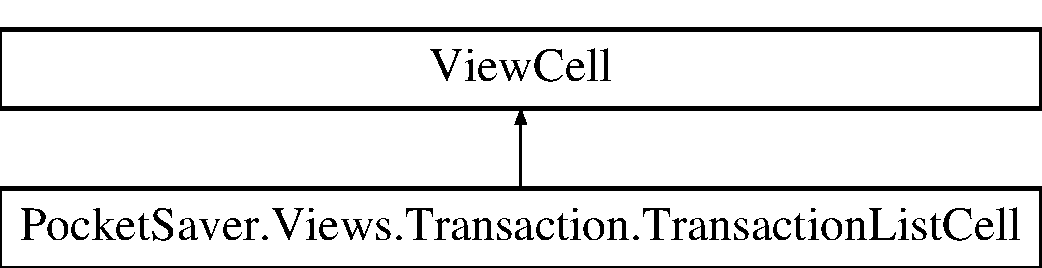
\includegraphics[height=2.000000cm]{class_pocket_saver_1_1_views_1_1_transaction_1_1_transaction_list_cell}
\end{center}
\end{figure}
\subsection*{Public Member Functions}
\begin{DoxyCompactItemize}
\item 
\hyperlink{class_pocket_saver_1_1_views_1_1_transaction_1_1_transaction_list_cell_a26039352cfde76eb1bca9b6c2141fae1}{Transaction\+List\+Cell} ()
\begin{DoxyCompactList}\small\item\em Constructor for the \hyperlink{class_pocket_saver_1_1_views_1_1_transaction_1_1_transaction_list_cell}{Transaction\+List\+Cell} which initializes all necessary components of the View\+Cell \end{DoxyCompactList}\end{DoxyCompactItemize}
\subsection*{Static Public Attributes}
\begin{DoxyCompactItemize}
\item 
static readonly Bindable\+Property {\bfseries Category\+Property}
\item 
static readonly Bindable\+Property {\bfseries Comment\+Property}
\item 
static readonly Bindable\+Property {\bfseries Date\+Property}
\item 
static readonly Bindable\+Property {\bfseries Purchase\+Amount\+Property}
\end{DoxyCompactItemize}
\subsection*{Protected Member Functions}
\begin{DoxyCompactItemize}
\item 
\mbox{\Hypertarget{class_pocket_saver_1_1_views_1_1_transaction_1_1_transaction_list_cell_a90e43ae65385f8f8e36d075798463d12}\label{class_pocket_saver_1_1_views_1_1_transaction_1_1_transaction_list_cell_a90e43ae65385f8f8e36d075798463d12}} 
override void {\bfseries On\+Binding\+Context\+Changed} ()
\end{DoxyCompactItemize}
\subsection*{Properties}
\begin{DoxyCompactItemize}
\item 
\mbox{\Hypertarget{class_pocket_saver_1_1_views_1_1_transaction_1_1_transaction_list_cell_a5cd6915c7c80aa41c2c7ad0b8f931c92}\label{class_pocket_saver_1_1_views_1_1_transaction_1_1_transaction_list_cell_a5cd6915c7c80aa41c2c7ad0b8f931c92}} 
string {\bfseries Category}\hspace{0.3cm}{\ttfamily  \mbox{[}get, set\mbox{]}}
\item 
\mbox{\Hypertarget{class_pocket_saver_1_1_views_1_1_transaction_1_1_transaction_list_cell_aa5cd06e831b18763e1dc0c56f61c6298}\label{class_pocket_saver_1_1_views_1_1_transaction_1_1_transaction_list_cell_aa5cd06e831b18763e1dc0c56f61c6298}} 
string {\bfseries Comment}\hspace{0.3cm}{\ttfamily  \mbox{[}get, set\mbox{]}}
\item 
\mbox{\Hypertarget{class_pocket_saver_1_1_views_1_1_transaction_1_1_transaction_list_cell_acceed74c5cc44e2e8caad5a5e8053efe}\label{class_pocket_saver_1_1_views_1_1_transaction_1_1_transaction_list_cell_acceed74c5cc44e2e8caad5a5e8053efe}} 
Date\+Time {\bfseries Date}\hspace{0.3cm}{\ttfamily  \mbox{[}get, set\mbox{]}}
\item 
\mbox{\Hypertarget{class_pocket_saver_1_1_views_1_1_transaction_1_1_transaction_list_cell_a758e9ee37c5208cacbd73a68433b8c58}\label{class_pocket_saver_1_1_views_1_1_transaction_1_1_transaction_list_cell_a758e9ee37c5208cacbd73a68433b8c58}} 
decimal {\bfseries Purchase\+Amount}\hspace{0.3cm}{\ttfamily  \mbox{[}get, set\mbox{]}}
\end{DoxyCompactItemize}


\subsection{Detailed Description}
Class for the \hyperlink{class_pocket_saver_1_1_views_1_1_transaction_1_1_transaction_list_cell}{Transaction\+List\+Cell} 



\subsection{Constructor \& Destructor Documentation}
\mbox{\Hypertarget{class_pocket_saver_1_1_views_1_1_transaction_1_1_transaction_list_cell_a26039352cfde76eb1bca9b6c2141fae1}\label{class_pocket_saver_1_1_views_1_1_transaction_1_1_transaction_list_cell_a26039352cfde76eb1bca9b6c2141fae1}} 
\index{Pocket\+Saver\+::\+Views\+::\+Transaction\+::\+Transaction\+List\+Cell@{Pocket\+Saver\+::\+Views\+::\+Transaction\+::\+Transaction\+List\+Cell}!Transaction\+List\+Cell@{Transaction\+List\+Cell}}
\index{Transaction\+List\+Cell@{Transaction\+List\+Cell}!Pocket\+Saver\+::\+Views\+::\+Transaction\+::\+Transaction\+List\+Cell@{Pocket\+Saver\+::\+Views\+::\+Transaction\+::\+Transaction\+List\+Cell}}
\subsubsection{\texorpdfstring{Transaction\+List\+Cell()}{TransactionListCell()}}
{\footnotesize\ttfamily Pocket\+Saver.\+Views.\+Transaction.\+Transaction\+List\+Cell.\+Transaction\+List\+Cell (\begin{DoxyParamCaption}{ }\end{DoxyParamCaption})\hspace{0.3cm}{\ttfamily [inline]}}



Constructor for the \hyperlink{class_pocket_saver_1_1_views_1_1_transaction_1_1_transaction_list_cell}{Transaction\+List\+Cell} which initializes all necessary components of the View\+Cell 



\subsection{Member Data Documentation}
\mbox{\Hypertarget{class_pocket_saver_1_1_views_1_1_transaction_1_1_transaction_list_cell_a03cf051a4c1e81e7ff5d3322ee8b02c7}\label{class_pocket_saver_1_1_views_1_1_transaction_1_1_transaction_list_cell_a03cf051a4c1e81e7ff5d3322ee8b02c7}} 
\index{Pocket\+Saver\+::\+Views\+::\+Transaction\+::\+Transaction\+List\+Cell@{Pocket\+Saver\+::\+Views\+::\+Transaction\+::\+Transaction\+List\+Cell}!Category\+Property@{Category\+Property}}
\index{Category\+Property@{Category\+Property}!Pocket\+Saver\+::\+Views\+::\+Transaction\+::\+Transaction\+List\+Cell@{Pocket\+Saver\+::\+Views\+::\+Transaction\+::\+Transaction\+List\+Cell}}
\subsubsection{\texorpdfstring{Category\+Property}{CategoryProperty}}
{\footnotesize\ttfamily readonly Bindable\+Property Pocket\+Saver.\+Views.\+Transaction.\+Transaction\+List\+Cell.\+Category\+Property\hspace{0.3cm}{\ttfamily [static]}}

{\bfseries Initial value\+:}
\begin{DoxyCode}
=
            BindableProperty.Create(\textcolor{stringliteral}{"Category"}, typeof(\textcolor{keywordtype}{string}), typeof(
      \hyperlink{class_pocket_saver_1_1_views_1_1_transaction_1_1_transaction_list_cell_a26039352cfde76eb1bca9b6c2141fae1}{TransactionListCell}), \textcolor{stringliteral}{"Category"})
\end{DoxyCode}
\mbox{\Hypertarget{class_pocket_saver_1_1_views_1_1_transaction_1_1_transaction_list_cell_a3c4421afb9db0560a2e0f9fc3d308e70}\label{class_pocket_saver_1_1_views_1_1_transaction_1_1_transaction_list_cell_a3c4421afb9db0560a2e0f9fc3d308e70}} 
\index{Pocket\+Saver\+::\+Views\+::\+Transaction\+::\+Transaction\+List\+Cell@{Pocket\+Saver\+::\+Views\+::\+Transaction\+::\+Transaction\+List\+Cell}!Comment\+Property@{Comment\+Property}}
\index{Comment\+Property@{Comment\+Property}!Pocket\+Saver\+::\+Views\+::\+Transaction\+::\+Transaction\+List\+Cell@{Pocket\+Saver\+::\+Views\+::\+Transaction\+::\+Transaction\+List\+Cell}}
\subsubsection{\texorpdfstring{Comment\+Property}{CommentProperty}}
{\footnotesize\ttfamily readonly Bindable\+Property Pocket\+Saver.\+Views.\+Transaction.\+Transaction\+List\+Cell.\+Comment\+Property\hspace{0.3cm}{\ttfamily [static]}}

{\bfseries Initial value\+:}
\begin{DoxyCode}
=
            BindableProperty.Create(\textcolor{stringliteral}{"Comment"}, typeof(\textcolor{keywordtype}{string}), typeof(
      \hyperlink{class_pocket_saver_1_1_views_1_1_transaction_1_1_transaction_list_cell_a26039352cfde76eb1bca9b6c2141fae1}{TransactionListCell}), \textcolor{stringliteral}{"Comment"})
\end{DoxyCode}
\mbox{\Hypertarget{class_pocket_saver_1_1_views_1_1_transaction_1_1_transaction_list_cell_a12b30ce09e98a1fbbd57ab148e8d4700}\label{class_pocket_saver_1_1_views_1_1_transaction_1_1_transaction_list_cell_a12b30ce09e98a1fbbd57ab148e8d4700}} 
\index{Pocket\+Saver\+::\+Views\+::\+Transaction\+::\+Transaction\+List\+Cell@{Pocket\+Saver\+::\+Views\+::\+Transaction\+::\+Transaction\+List\+Cell}!Date\+Property@{Date\+Property}}
\index{Date\+Property@{Date\+Property}!Pocket\+Saver\+::\+Views\+::\+Transaction\+::\+Transaction\+List\+Cell@{Pocket\+Saver\+::\+Views\+::\+Transaction\+::\+Transaction\+List\+Cell}}
\subsubsection{\texorpdfstring{Date\+Property}{DateProperty}}
{\footnotesize\ttfamily readonly Bindable\+Property Pocket\+Saver.\+Views.\+Transaction.\+Transaction\+List\+Cell.\+Date\+Property\hspace{0.3cm}{\ttfamily [static]}}

{\bfseries Initial value\+:}
\begin{DoxyCode}
=
            BindableProperty.Create(\textcolor{stringliteral}{"Date"}, typeof(DateTime?), typeof(
      \hyperlink{class_pocket_saver_1_1_views_1_1_transaction_1_1_transaction_list_cell_a26039352cfde76eb1bca9b6c2141fae1}{TransactionListCell}), null)
\end{DoxyCode}
\mbox{\Hypertarget{class_pocket_saver_1_1_views_1_1_transaction_1_1_transaction_list_cell_aabf6dc4177c779f522a46f61f843ed49}\label{class_pocket_saver_1_1_views_1_1_transaction_1_1_transaction_list_cell_aabf6dc4177c779f522a46f61f843ed49}} 
\index{Pocket\+Saver\+::\+Views\+::\+Transaction\+::\+Transaction\+List\+Cell@{Pocket\+Saver\+::\+Views\+::\+Transaction\+::\+Transaction\+List\+Cell}!Purchase\+Amount\+Property@{Purchase\+Amount\+Property}}
\index{Purchase\+Amount\+Property@{Purchase\+Amount\+Property}!Pocket\+Saver\+::\+Views\+::\+Transaction\+::\+Transaction\+List\+Cell@{Pocket\+Saver\+::\+Views\+::\+Transaction\+::\+Transaction\+List\+Cell}}
\subsubsection{\texorpdfstring{Purchase\+Amount\+Property}{PurchaseAmountProperty}}
{\footnotesize\ttfamily readonly Bindable\+Property Pocket\+Saver.\+Views.\+Transaction.\+Transaction\+List\+Cell.\+Purchase\+Amount\+Property\hspace{0.3cm}{\ttfamily [static]}}

{\bfseries Initial value\+:}
\begin{DoxyCode}
=
            BindableProperty.Create(\textcolor{stringliteral}{"PurchaseAmount"}, typeof(decimal), typeof(
      \hyperlink{class_pocket_saver_1_1_views_1_1_transaction_1_1_transaction_list_cell_a26039352cfde76eb1bca9b6c2141fae1}{TransactionListCell}), 0.00m)
\end{DoxyCode}


The documentation for this class was generated from the following file\+:\begin{DoxyCompactItemize}
\item 
C\+:/\+Users/\+Mevin/\+Pocket\+Saver/src/\+Pocket\+Saver/\+Pocket\+Saver/\+Pocket\+Saver/\+Views/\+Transaction/Transaction\+List\+Cell.\+cs\end{DoxyCompactItemize}

\hypertarget{class_pocket_saver_1_1_views_1_1_transaction_1_1_transaction_list_page}{}\section{Pocket\+Saver.\+Views.\+Transaction.\+Transaction\+List\+Page Class Reference}
\label{class_pocket_saver_1_1_views_1_1_transaction_1_1_transaction_list_page}\index{Pocket\+Saver.\+Views.\+Transaction.\+Transaction\+List\+Page@{Pocket\+Saver.\+Views.\+Transaction.\+Transaction\+List\+Page}}


Class for the \hyperlink{class_pocket_saver_1_1_views_1_1_transaction_1_1_transaction_list_page}{Transaction\+List\+Page} of the \hyperlink{namespace_pocket_saver}{Pocket\+Saver} Mobile Application.  


Inheritance diagram for Pocket\+Saver.\+Views.\+Transaction.\+Transaction\+List\+Page\+:\begin{figure}[H]
\begin{center}
\leavevmode
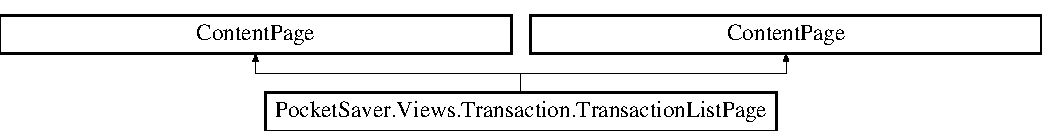
\includegraphics[height=1.761006cm]{class_pocket_saver_1_1_views_1_1_transaction_1_1_transaction_list_page}
\end{center}
\end{figure}
\subsection*{Public Member Functions}
\begin{DoxyCompactItemize}
\item 
\hyperlink{class_pocket_saver_1_1_views_1_1_transaction_1_1_transaction_list_page_ac38869636ca8f6dc89b37145bb838733}{Transaction\+List\+Page} ()
\begin{DoxyCompactList}\small\item\em Constructor for the \hyperlink{class_pocket_saver_1_1_views_1_1_transaction_1_1_transaction_list_page}{Transaction\+List\+Page} which initializes the Transaction\+View\+Model and defines the listview item selection. \end{DoxyCompactList}\end{DoxyCompactItemize}
\subsection*{Protected Member Functions}
\begin{DoxyCompactItemize}
\item 
override async void \hyperlink{class_pocket_saver_1_1_views_1_1_transaction_1_1_transaction_list_page_a8af1a929634ca8eb26dadd56d6d02fc4}{On\+Appearing} ()
\begin{DoxyCompactList}\small\item\em On\+Appearing Method which is used to declare variables and methods to be called upon the page appearing. \end{DoxyCompactList}\end{DoxyCompactItemize}


\subsection{Detailed Description}
Class for the \hyperlink{class_pocket_saver_1_1_views_1_1_transaction_1_1_transaction_list_page}{Transaction\+List\+Page} of the \hyperlink{namespace_pocket_saver}{Pocket\+Saver} Mobile Application. 



\subsection{Constructor \& Destructor Documentation}
\mbox{\Hypertarget{class_pocket_saver_1_1_views_1_1_transaction_1_1_transaction_list_page_ac38869636ca8f6dc89b37145bb838733}\label{class_pocket_saver_1_1_views_1_1_transaction_1_1_transaction_list_page_ac38869636ca8f6dc89b37145bb838733}} 
\index{Pocket\+Saver\+::\+Views\+::\+Transaction\+::\+Transaction\+List\+Page@{Pocket\+Saver\+::\+Views\+::\+Transaction\+::\+Transaction\+List\+Page}!Transaction\+List\+Page@{Transaction\+List\+Page}}
\index{Transaction\+List\+Page@{Transaction\+List\+Page}!Pocket\+Saver\+::\+Views\+::\+Transaction\+::\+Transaction\+List\+Page@{Pocket\+Saver\+::\+Views\+::\+Transaction\+::\+Transaction\+List\+Page}}
\subsubsection{\texorpdfstring{Transaction\+List\+Page()}{TransactionListPage()}}
{\footnotesize\ttfamily Pocket\+Saver.\+Views.\+Transaction.\+Transaction\+List\+Page.\+Transaction\+List\+Page (\begin{DoxyParamCaption}{ }\end{DoxyParamCaption})\hspace{0.3cm}{\ttfamily [inline]}}



Constructor for the \hyperlink{class_pocket_saver_1_1_views_1_1_transaction_1_1_transaction_list_page}{Transaction\+List\+Page} which initializes the Transaction\+View\+Model and defines the listview item selection. 



\subsection{Member Function Documentation}
\mbox{\Hypertarget{class_pocket_saver_1_1_views_1_1_transaction_1_1_transaction_list_page_a8af1a929634ca8eb26dadd56d6d02fc4}\label{class_pocket_saver_1_1_views_1_1_transaction_1_1_transaction_list_page_a8af1a929634ca8eb26dadd56d6d02fc4}} 
\index{Pocket\+Saver\+::\+Views\+::\+Transaction\+::\+Transaction\+List\+Page@{Pocket\+Saver\+::\+Views\+::\+Transaction\+::\+Transaction\+List\+Page}!On\+Appearing@{On\+Appearing}}
\index{On\+Appearing@{On\+Appearing}!Pocket\+Saver\+::\+Views\+::\+Transaction\+::\+Transaction\+List\+Page@{Pocket\+Saver\+::\+Views\+::\+Transaction\+::\+Transaction\+List\+Page}}
\subsubsection{\texorpdfstring{On\+Appearing()}{OnAppearing()}}
{\footnotesize\ttfamily override async void Pocket\+Saver.\+Views.\+Transaction.\+Transaction\+List\+Page.\+On\+Appearing (\begin{DoxyParamCaption}{ }\end{DoxyParamCaption})\hspace{0.3cm}{\ttfamily [inline]}, {\ttfamily [protected]}}



On\+Appearing Method which is used to declare variables and methods to be called upon the page appearing. 



The documentation for this class was generated from the following files\+:\begin{DoxyCompactItemize}
\item 
C\+:/\+Users/\+Mevin/\+Pocket\+Saver/src/\+Pocket\+Saver/\+Pocket\+Saver/\+Pocket\+Saver/obj/\+Debug/Pocket\+Saver.\+Views.\+Transaction.\+Transaction\+List\+Page.\+xaml.\+g.\+cs\item 
C\+:/\+Users/\+Mevin/\+Pocket\+Saver/src/\+Pocket\+Saver/\+Pocket\+Saver/\+Pocket\+Saver/\+Views/\+Transaction/Transaction\+List\+Page.\+xaml.\+cs\end{DoxyCompactItemize}

\hypertarget{class_pocket_saver_1_1_models_1_1_transaction_model}{}\section{Pocket\+Saver.\+Models.\+Transaction\+Model Class Reference}
\label{class_pocket_saver_1_1_models_1_1_transaction_model}\index{Pocket\+Saver.\+Models.\+Transaction\+Model@{Pocket\+Saver.\+Models.\+Transaction\+Model}}


Class for the \hyperlink{class_pocket_saver_1_1_models_1_1_transaction_model}{Transaction\+Model} Object to be used throughout the application.  


\subsection*{Properties}
\begin{DoxyCompactItemize}
\item 
\mbox{\Hypertarget{class_pocket_saver_1_1_models_1_1_transaction_model_a66392d6b5d8574181ea9db65bf2b3308}\label{class_pocket_saver_1_1_models_1_1_transaction_model_a66392d6b5d8574181ea9db65bf2b3308}} 
string {\bfseries \+\_\+id}\hspace{0.3cm}{\ttfamily  \mbox{[}get, set\mbox{]}}
\item 
\mbox{\Hypertarget{class_pocket_saver_1_1_models_1_1_transaction_model_a8ea4b5bbb326f50ceb55a8ad8503a0f3}\label{class_pocket_saver_1_1_models_1_1_transaction_model_a8ea4b5bbb326f50ceb55a8ad8503a0f3}} 
string {\bfseries Category}\hspace{0.3cm}{\ttfamily  \mbox{[}get, set\mbox{]}}
\item 
\mbox{\Hypertarget{class_pocket_saver_1_1_models_1_1_transaction_model_a41781f1e8223daefb26255ecdac60724}\label{class_pocket_saver_1_1_models_1_1_transaction_model_a41781f1e8223daefb26255ecdac60724}} 
Date\+Time {\bfseries Date}\hspace{0.3cm}{\ttfamily  \mbox{[}get, set\mbox{]}}
\item 
\mbox{\Hypertarget{class_pocket_saver_1_1_models_1_1_transaction_model_a2332c4ad1344019a701fea92f2bc415e}\label{class_pocket_saver_1_1_models_1_1_transaction_model_a2332c4ad1344019a701fea92f2bc415e}} 
decimal {\bfseries Purchase\+Amount}\hspace{0.3cm}{\ttfamily  \mbox{[}get, set\mbox{]}}
\item 
\mbox{\Hypertarget{class_pocket_saver_1_1_models_1_1_transaction_model_abb22b0967b66b4e99788edfdeee157a0}\label{class_pocket_saver_1_1_models_1_1_transaction_model_abb22b0967b66b4e99788edfdeee157a0}} 
string {\bfseries Comment}\hspace{0.3cm}{\ttfamily  \mbox{[}get, set\mbox{]}}
\end{DoxyCompactItemize}


\subsection{Detailed Description}
Class for the \hyperlink{class_pocket_saver_1_1_models_1_1_transaction_model}{Transaction\+Model} Object to be used throughout the application. 



The documentation for this class was generated from the following file\+:\begin{DoxyCompactItemize}
\item 
C\+:/\+Users/\+Mevin/\+Pocket\+Saver/src/\+Pocket\+Saver/\+Pocket\+Saver/\+Pocket\+Saver/\+Services/\+Models/Transaction\+Model.\+cs\end{DoxyCompactItemize}

\hypertarget{class_pocket_saver_1_1_view_models_1_1_transaction_1_1_transaction_view_model}{}\section{Pocket\+Saver.\+View\+Models.\+Transaction.\+Transaction\+View\+Model Class Reference}
\label{class_pocket_saver_1_1_view_models_1_1_transaction_1_1_transaction_view_model}\index{Pocket\+Saver.\+View\+Models.\+Transaction.\+Transaction\+View\+Model@{Pocket\+Saver.\+View\+Models.\+Transaction.\+Transaction\+View\+Model}}
Inheritance diagram for Pocket\+Saver.\+View\+Models.\+Transaction.\+Transaction\+View\+Model\+:\begin{figure}[H]
\begin{center}
\leavevmode
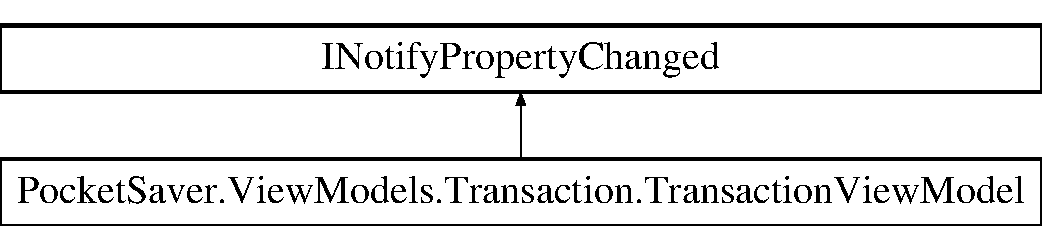
\includegraphics[height=2.000000cm]{class_pocket_saver_1_1_view_models_1_1_transaction_1_1_transaction_view_model}
\end{center}
\end{figure}
\subsection*{Static Public Member Functions}
\begin{DoxyCompactItemize}
\item 
\mbox{\Hypertarget{class_pocket_saver_1_1_view_models_1_1_transaction_1_1_transaction_view_model_a18c3f058a5098c06cb7784ea7e5c8537}\label{class_pocket_saver_1_1_view_models_1_1_transaction_1_1_transaction_view_model_a18c3f058a5098c06cb7784ea7e5c8537}} 
static async Task {\bfseries Refresh\+List} ()
\end{DoxyCompactItemize}
\subsection*{Static Public Attributes}
\begin{DoxyCompactItemize}
\item 
\mbox{\Hypertarget{class_pocket_saver_1_1_view_models_1_1_transaction_1_1_transaction_view_model_a5e19ca45b1a5803cbb1ab7b506ca9820}\label{class_pocket_saver_1_1_view_models_1_1_transaction_1_1_transaction_view_model_a5e19ca45b1a5803cbb1ab7b506ca9820}} 
static Observable\+Collection$<$ \hyperlink{class_pocket_saver_1_1_models_1_1_transaction_model}{Transaction\+Model} $>$ {\bfseries transaction\+Datum} = new Observable\+Collection$<$\hyperlink{class_pocket_saver_1_1_models_1_1_transaction_model}{Transaction\+Model}$>$()
\end{DoxyCompactItemize}
\subsection*{Protected Member Functions}
\begin{DoxyCompactItemize}
\item 
\mbox{\Hypertarget{class_pocket_saver_1_1_view_models_1_1_transaction_1_1_transaction_view_model_a322474d9390bb1c47b9b73f76e2aa519}\label{class_pocket_saver_1_1_view_models_1_1_transaction_1_1_transaction_view_model_a322474d9390bb1c47b9b73f76e2aa519}} 
void {\bfseries Notify\+Property\+Changed} (String info)
\end{DoxyCompactItemize}
\subsection*{Properties}
\begin{DoxyCompactItemize}
\item 
\mbox{\Hypertarget{class_pocket_saver_1_1_view_models_1_1_transaction_1_1_transaction_view_model_a05bc69b164fa7d830f71a76fbbc0aab3}\label{class_pocket_saver_1_1_view_models_1_1_transaction_1_1_transaction_view_model_a05bc69b164fa7d830f71a76fbbc0aab3}} 
bool {\bfseries is\+Refreshing}\hspace{0.3cm}{\ttfamily  \mbox{[}get, set\mbox{]}}
\end{DoxyCompactItemize}
\subsection*{Events}
\begin{DoxyCompactItemize}
\item 
\mbox{\Hypertarget{class_pocket_saver_1_1_view_models_1_1_transaction_1_1_transaction_view_model_a258c2b7249a3e23d71d6669ef91d46bd}\label{class_pocket_saver_1_1_view_models_1_1_transaction_1_1_transaction_view_model_a258c2b7249a3e23d71d6669ef91d46bd}} 
Property\+Changed\+Event\+Handler {\bfseries Property\+Changed}
\end{DoxyCompactItemize}


The documentation for this class was generated from the following file\+:\begin{DoxyCompactItemize}
\item 
C\+:/\+Users/\+Mevin/\+Pocket\+Saver/src/\+Pocket\+Saver/\+Pocket\+Saver/\+Pocket\+Saver/\+View\+Models/\+Transaction/Transaction\+View\+Model.\+cs\end{DoxyCompactItemize}

%--- End generated contents ---

% Index
\backmatter
\newpage
\phantomsection
\clearemptydoublepage
\addcontentsline{toc}{chapter}{Index}
\printindex

\end{document}
